\documentclass{book}
\usepackage{xcolor}
\usepackage{color}
\usepackage[spanish]{babel}
\usepackage{graphicx}
\usepackage{hyperref}
\usepackage{booktabs}
\usepackage{varwidth}
\usepackage{caption}
\usepackage{multirow}
\usepackage{textcomp}
\usepackage{url}
\usepackage{amsmath}
\usepackage[inline]{enumitem}
\usepackage{todonotes}
\usepackage{enumitem,amssymb}
\newlist{todolist}{itemize}{2}
\setlist[todolist]{label=$\square$}
\usepackage{color}
\usepackage{rotating}

\newcommand{\emc}[1]{\textcolor{blue}{#1}}
\newenvironment{naranja}{\par\color{orange}}{\par}

\begin{document}

\title{Cómo escribir la memoria de tu TFG del Grado de Ingeniería Informática y presentarlo sin morir en el intento (tentativo)}
\author{Tus Nombres}
\date{\today}
\maketitle

\tableofcontents
\listoftables
\listoffigures

% Incluye los archivos de los capítulos
\chapter{Prólogo}

Todavía no está terminado. Terminarlo al final de la revisión completa del libro.

% [Autores: lo podemos hacer al final todos]
\textit{Aviso 1}: en este libro se refleja la  “opinión” de un conjunto de profesores a partir de su experiencia y conocimientos académicos, así como su experiencia, tanto como tutores como evaluadores. Es un conjunto de recomendaciones, sugerencias y buenas prácticas que en ningún momento garantizan que, tras seguirlas, se obtengan buenos resultados y además puede haber efectos secundarios ;-) 

\textit{Aviso 2}: al igual que las distribuciones normales tienen una media representativa, las colas de la distribución siguen siendo valores correctos de la distribución. En este documento hemos intentado comentar la media con una amplia desviación, no obstante, la tupla formada por (TFG, alumno, profesor, tema) puede caer en los extremos de la distribución y seguir siendo normal. En otras palabras, si consideras que tu TFG no se acomoda a lo aquí presentado, no te preocupes, y si sabes responder el porqué, seguro que estará en el extremo de los excelentes. 

\textit{Aviso 3}: este libro ha intentado realizar un uso no sexista del lenguaje, haciendo uso indistinto de  tutor/tutora, profesor/profesora y alumno/alumna, empleando sustantivos genéricos como estudiante, estudiantado, alumnado o profesorado, pronombres sin marcas de género (quienes), entre otras alternativas al lenguaje no sexista. Si algo se nos ha pasado, pedimos disculpas.


\chapter{Introducción}
\label{cap:Introducción}
%Juanma
%Iniciativas previas: \url{https://drive.google.com/drive/folders/1WMPwX1v7IhG88bJYLXDgm4Zp6a_pCCHh}

Todavía no está terminado. Terminarlo al final de la revisión completa del libro.


Este libro queda dividido en los siguientes capítulos: en el capítulo \ref{cap:Recomendaciones} se ofrece, para empezar, información general sobre el proceso de asignación del TFG, contexto general que debes conocer antes de comenzar a trabajar, así como pautas y recomendaciones de trabajo para ayudarte en el desarrollo del proyecto. El capítulo \ref{cap:EstructuraMemoria} establece una propuesta de estructura general de la memoria, indicando cada una de las partes que la compone, para que tengas una idea general de cómo organizar este documento. El siguiente capítulo, el \ref{cap:IntroducciónTFG}, se centra en describir el contenido del capítulo de introducción, ofreciendo tanto una posible estructura del mismo como consejos para su elaboración. El capítulo \ref{cap:RevisionEstadoDelArte} pasa a describir cómo se debe hacer una revisión del estado del arte, parte fundamental en cualquier memoria de TFG. Un elemento importante en todo proyecto es la planificación y el presupuesto, y en el capítulo \ref{cap:PlanificacionPresupuesto} damos algunos consejos para su elaboración. Seguidamente, en el capítulo \ref{cap:Tipologías} se presentan los cuatro tipos de TFG principales: de desarrollo, experimental, investigación y de revisión. Recomendaciones sobre cómo abordar la confección de las conclusiones y los trabajos futuros se incluyen en el capítulo \ref{cap:Conclusiones}. El capítulo \ref{cap:bibliografia} aborda asuntos relacionados con la bibliografía y cómo referenciarla en la memoria y el siguiente, el capítulo \ref{cap:anexos} hace lo propio con los anexos que puedes incluir en la memora.  Una vez que la esta está terminada, en el capítulo \ref{cap:Revisión} se muestra una lista de comprobaciones que deberías hacer para estar seguros de que la memoria alcanza el mínimo de calidad exigible. Los dos capítulos siguientes, y últimos, el \ref{cap:elaboraciónPresentación} y \ref{cap:defensa}, se centran en la presentación y en la defensa, respectivamente, aconsejando sobre cómo montar la primera y cómo afrontar la segunda. Y como no podía ser de otra manera, este libro finaliza con un capítulo de anexos 
\chapter{Recomendaciones generales}
\label{cap:Recomendaciones}

% [Autores: María José Rodríguez Fórtiz, Juanma, Alberto]
%%%%%%%%%%%%%%%%%%%%%%%%%%%%%%%%%%%%%%%%%%%%%%
%%%%%%%%%%%%%%%%%%%%%%%%%%%%%%%%%%%%%%%%%%%%%%

\section{Sobre la elección del TFG}

%%%%%%%%%%%%%%%%%%%%%%%%%%%%%%%%%%%%%%%%%%%%%%
%%%%%%%%%%%%%%%%%%%%%%%%%%%%%%%%%%%%%%%%%%%%%%

Ya estás en cuarto del grado y en ese momento aparece una asignatura de segundo semestre que se denomina Trabajo Fin de Grado de la cual sabes poco salvo que tienes que realizar un proyecto. Te matriculas en ella y seguidamente se te vienen a la cabeza una serie de cuestiones, entre las que estarán seguro algunas de estas: ¿y ahora qué hago? ¿qué TFG elijo? ¿con qué profesor/a? Normalmente vienen seguidas de un tiempo de cierta incertidumbre y algo de ansiedad, hasta que por fin consigues tener un tutor o tutora y un proyecto en el que ponerte a trabajar. En esta sección vamos a hacerte algunas recomendaciones para ayudarte a responderlas y a que este proceso previo sea más llevadero.

Antes de comenzar, comentarte que existen dos fases en la asignación de TFGs. En la primera, el estudiante y el docente llegan a un acuerdo y el segundo hace una preasignación del TFG al estudiante. En la segunda, el centro publica una lista de TFGs que han propuesto los docentes y los estudiantes que no tienen TFGs preasignados en la primera fase, eligen por orden de preferencia propuestas de TFGs. La Escuela se encarga de realizar la asignación aplicando los criterios que estén vigentes en el momento (normalmente expediente académico de los estudiantes). Normalmente este proceso se realiza en octubre y en febrero o marzo. Todo esto bajo la premisa de que estés matriculado en la asignatura. Que no se te olvide. Aunque también puede darse el caso de buscar TFG aunque no lo estés, pero quieras ir avanzando en el desarrollo del mismo. 

La primera sugerencia que te hacemos es que seas proactivo en la elección de la temática del TFG. No esperes a la segunda fase y busca tu TFG en la primera. No seas tímido y propón cambios a la idea que esté propuesta por el profesor o, incluso, piensa en alternativas completamente alejadas. El profesorado puede no querer cambiar, pero por lo general, a la hora de proponer TFG hay bastante flexibilidad.

Respecto a cuando empezar, aunque es una asignatura de segundo semestre muchos estudiantes comienzan a buscar y trabajar en su TFG en el primer semestre o a final de tercero. Así, hay ocasiones en que los estudiantes tenéis muy claro qué quieres hacer en vuestro trabajo fin de carrera. Esto puede deberse a múltiples situaciones. Por ejemplo, imagina algunas de estas: desde algunos cursos antes tienes entre manos el desarrollo de un proyecto personal y consideras que el TFG puede ser un contexto idóneo para avanzarlo; o bien, lo que tienes es una idea de proyecto personal y esta asignatura te plantea una excusa perfecta para llevarlo a cabo. También puede ser que hayas aprendido alguna tecnología o aplicación en alguna asignatura y estás motivado para trabajar en ella. Pero no sólo tienen que ser proyectos personales, sino que también entra en juego tu mentalidad emprendedora y has detectado un nicho donde el producto o servicio que obtengas como salida de tu TFG es susceptible de ser comercializado. Y también están los proyectos profesionales. Es habitual que cuando llegues a cuarto estés haciendo tus prácticas en empresa o incluso que ya estés contratado. Y en ese entorno profesional pueden existir desafíos o temáticas en las que estás trabajando en tu empresa, o podrías trabajar, y que serían susceptibles de ser abordados en tu TFG.

Asumiendo que estás en una de estas situaciones, o en cualquier otra en la que ya tengas una idea clara de lo que quieres hacer, el primer paso que tienes que dar es sentarte tranquilamente y escribir una descripción del problema que deseas abordar, lo suficientemente completa para que un posible lector tenga una idea bastante clara de tu propuesta tras leerla. 

El siguiente paso será la búsqueda del docente que te dirigirá el trabajo. Aquí existen varias situaciones: la primera es que tienes cierta confianza con algún profesor o cierta afinidad personal, te cae bien o crees que puedes trabajar bien con él. En ese caso, concierta una tutoría y exponle tu idea y dile directamente que te gustaría que fuera la persona que te tutorice, explicándole las razones. Ese documento que habías hecho, házselo llegar previamente a la tutoría con objeto de que conozca tu idea y puedas explicársela con cierto conocimiento de la misma por su parte y resolver las dudas que te pueda plantear. Si te dice que sí, has triunfado y, a partir de ahí, os podéis poner a trabajar, seguramente en una fase inicial donde concretéis detalles del proyecto. Si te dice que no, busca otro profesor. Podría ser interesante que hicieras una lista con los docentes a los que plantearle la dirección, ordenada por preferencia. La otra alternativa para solicitar a un docente que sea la persona que te tutorice es que sea experto en la temática de tu idea. En este caso, busca qué profesores investigan en ese tema o imparten clases en asignaturas relacionadas, y procede de la misma forma explicada. Para ello, inspecciona las guías docentes de las asignaturas afines a la temática de tu idea, mira los sitios web de los departamentos y de los grupos de investigación para encontrar docentes que sean expertos en temas relacionados con tu idea. 

Si no tienes una idea clara, pero sí sabes con certeza con qué tutor querrías trabajar, ve a verlo y dile que quieres hacer el TFG con él y si existe la posibilidad de que te proponga algún tema que pueda ser de tu interés. Si dice que sí, y hay alguna propuesta que te guste, ya puedes empezar a trabajar. Si dice que no o ninguna de las propuestas te interesan, entonces echa mano del siguiente profesor de la lista.

Otra opción que existe cuando no se tiene una idea clara de lo que hacer y tampoco se tiene claro con quién hacerlo es acudir a la web donde se publican las propuestas de TFGs para ese curso. Los docentes suelen publicar sus propuesta con objeto de darlas a conocer y que los estudiantes las puedan elegir. Mira las que te gustan y cítate con los docentes para que te las expliquen con más detalle. Cuando encuentres una propuesta que te guste, solicítasela al profesor. 

Todo lo anteriormente indicado se aplica en la fase de preasignación. Si por cualquier causa (despiste, falta de iniciativa, dudas, etc.) no se te ha asignado un TFG en esta fase, pasarías a la segunda. Como ya hemos comentado, tendrás que ordenar los TFGs propuestos en orden decreciente de interés, y esperar que la Escuela te asigne alguno de los que has seleccionado. En este caso, no hagas la ordenación al tuntún ni introduzcas en la lista todos los TFGs, sino que selecciona los que verdaderamente te interesen. Habla con los tutores de los que te gustan y pídeles que te den detalles para que puedas hacer una ordenación informada según tus gustos, combinando tanto la temática del TFG como el docente que lo propone. Y a partir de ahí, a cruzar los dedos para que el que has puesto como primero, o alguno de los primeros puestos,  sea el que se te asigne. Corres el peligro te den uno situado al final de esa lista. Esto tiene al menos dos inconvenientes: puede ser que no te motive la propuesta o que la persona que te tutoriza que te ha tocado no sea santo de tu devoción. En ese caso, tendrás que plantearte si seguir para delante con lo que te ha tocado o dejar el TFG para el curso siguiente (no tiene que ser junio, también puede ser la convocatoria extraordinaria, normalmente en noviembre) y buscar o proponer tú el tema de tu TFG con tiempo.

Como podrás imaginar, siempre es mejor que tengas tú la iniciativa y buscar una proyecto que te motive y un tutor con el que estés a gusto trabajando. Piensa que las horas las tienes que trabajar igualmente, así que mucho mejor si lo haces persiguiendo un objetivo que te interese y motive.

También es importante, si optas por la la opción proactiva, es el momento en el que comienzas a moverte y a realizar contactos con el profesorado. Si lo dejas para muy tarde, seguramente éstos estén ya cargados de TFGs y puedas recibir varias negativas a tus propuestas o los propuestos que te interesan ya hayan sido preasignados. Esta es la razón por la que te recomendamos que comiences el proceso de búsqueda de TFG lo antes posible. Hay estudiantes que a final de tercero, antes de vacaciones, están buscando ya; otros justo a la vuelta, en septiembre y algunos lo dejan para la asignación de noviembre. En este último caso, las opciones quedarán reducidas considerablemente, así que, cuanto antes, mejor.

En esas reuniones previas a la preasignación donde finalmente hay un acuerdo entre estudiante y docente, un aspecto muy relevante es la discusión del alcance del TFG y sus objetivos. En ellas tenéis que concretar cuáles serán las funcionalidades de los desarrollos asociados al TFG y qué objetivos os marcáis para el mismo. Estas negociaciones son importantes porque determinarán hasta dónde tendrás que llegar en tu proyecto. En este sentido, cuando se te preasigne asegúrate que tengas claro este alcance. Procura que, al definir estos objetivos, que sean realistas, y que consideres para que así sean, el tiempo que tienes disponible para trabajar en él y cuándo quieres tenerlo listo para entregarlo. Puedes ver un resumen de todo este proceso en la Figura  \ref{fg_diagrama_proceso}.

Ya para concluir esta sección, comentarte que la realización de un TFG es un proceso que te está entrenando para el ámbito profesional. Vas a realizar un trabajo que se asemejará al que realizarás cuando hayas terminado y estés contratado en una empresa. Aprovecha esta oportunidad para aprender nuevas metodologías, tecnologías, lenguajes, etc. que no has visto en el grado y que te puedan servir en la nueva fase profesional que se te abrirá en pocos meses. Además, es una magnífica carta de presentación en las entrevistas ya que podrán ver tu capacidad de trabajo y de aprendizaje de nuevos conceptos, cosa que permitirá diferenciarte de otros candidatos. Por tanto, te sugerimos que aproveches la oportunidad de realizar un TFG en el que aprendas muchas cosas y en una temática que te guste. 

Como nota final, recuerda que para presentarlo en la convocatoria extraordinaria de noviembre tienes que haberlo solicitado en la sede.ugr.es tal y como indica la web de la Escuela \url{https://grados.ugr.es/informatica/pages/infoacademica/tfggestion2}. Hay unos plazos para dicha solicitud, no dejes que se te pase.

% SUGERENCIA -> INFOGRAFÏA CON DIAGRAMA DE FLUJO DEL PROCESO
\begin{figure}[!ht]
\centering
    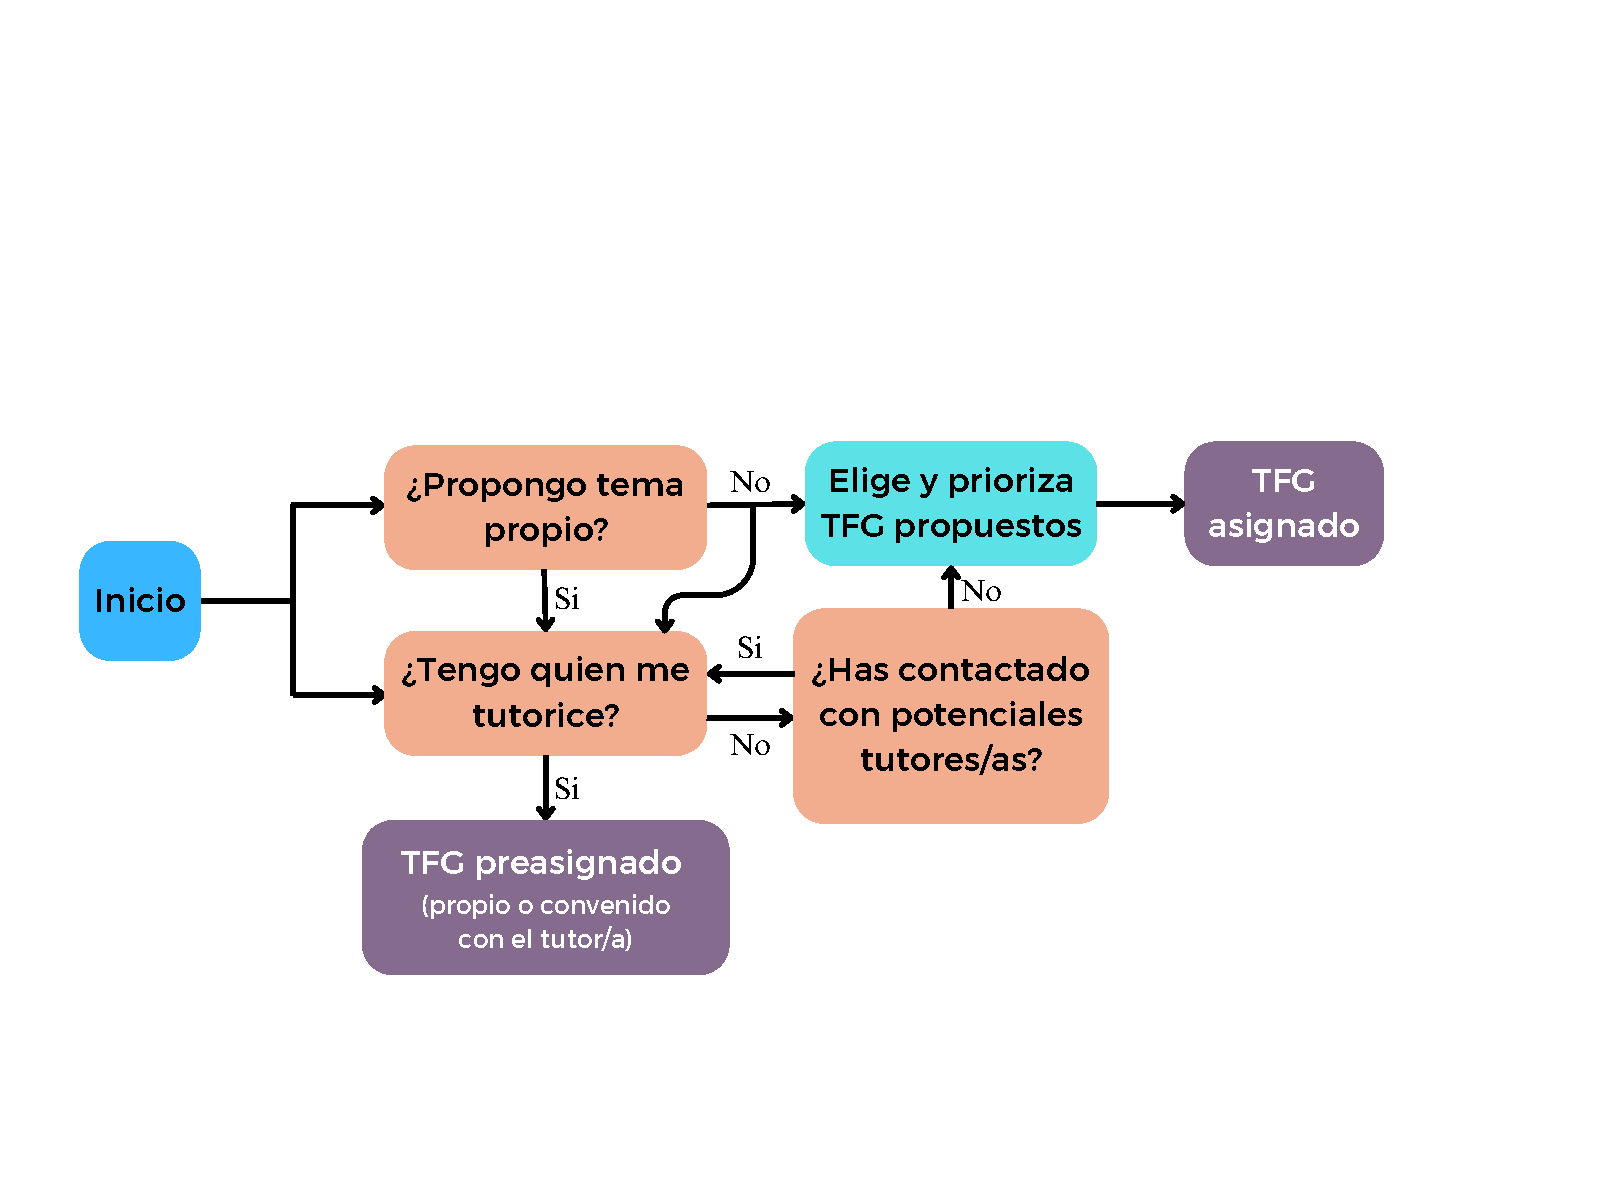
\includegraphics[scale=0.5]{images/DecisionTFG.pdf}
    \caption{Diagrama de flujo del proceso.}\label{fg_diagrama_proceso}
\end{figure}

%%%%%%%%%%%%%%%%%%%%%%%%%%%%%%%%%%%%%%%%%%%%%%
%%%%%%%%%%%%%%%%%%%%%%%%%%%%%%%%%%%%%%%%%%%%%%

\section{Sobre el desarrollo del proyecto}

%%%%%%%%%%%%%%%%%%%%%%%%%%%%%%%%%%%%%%%%%%%%%%
%%%%%%%%%%%%%%%%%%%%%%%%%%%%%%%%%%%%%%%%%%%%%%

En esta sección vamos a comentar aspectos fundamentales para el éxito de cualquier proyecto. Comenzaremos con la comunicación con la persona que te tutoriza, posteriormente con la disciplina y la pauta de trabajo (no es lo mismo caminar 1Km cada día durante 100 días que caminar 100Km en un día...), y cuestiones menos técnicas como aspectos éticos y de propiedad intelectual.

%%%%%%%%%%%%%%%%%%%%%%%%%%%%%%%%%%%%%%%%%%%%%%
\subsection{Reuniones con la persona que te tutoriza}%(María José)
%%%%%%%%%%%%%%%%%%%%%%%%%%%%%%%%%%%%%%%%%%%%%%

Durante el desarrollo del TFG debes mantener varias reuniones con la persona que te tutoriza con el objetivo de organizar y revisar tu trabajo. Las reuniones pueden ser presenciales u online, dependerá de ti y de la persona que te tutoriza.

En las primeras reuniones con la persona que te tutoriza, tal y como se ha comentado antes, debes consensuar el alcance y objetivos del proyecto. Un TFG debe ser un trabajo original, claro, riguroso, coherente, relevante, y pertinente. Por eso, te insistimos en que concretes bien y sin divagar cuál va a ser la orientación y aportación del trabajo desde el principio, qué se va a mejorar respecto a lo existente. En las reuniones iniciales también se debe proponer y seleccionar la metodología a seguir y cuál será la estructura de la memoria. Aunque luego pueda haber cambios, es interesante hacer el ejercicio a priori para tener una idea de cómo se va a desarrollar el trabajo.

En las siguientes reuniones la persona que te tutoriza puede ayudarte a resolver dudas, ir validando el desarrollo realizado, y corregirte lo que vayas escribiendo de la memoria, por ejemplo, indicándote el grado de profundidad al exponer los temas, o las mejores herramientas de diseño a utilizar. También puede sugerirte bibliografía para completar el estado del arte o contexto del trabajo o facilitarte materiales para el desarrollo. 

Te aconsejamos que te reúnas con la persona que te tutoriza con frecuencia, aunque esta varíe según tus otras ocupaciones en otras asignaturas o en tu trabajo, si ya lo tienes. Lo habitual es quedar de forma sistemática con ella en diferentes momentos considerando la metodología de trabajo que estés siguiendo, al acabar un paso, fase o tarea y antes de empezar el siguiente. Eso te obligará a ser más constante en tu trabajo ya que sabes que tienes que rendir cuentas de lo que has hecho en ese tiempo. Así, por ejemplo, es frecuente planificar pasos, fases o tareas de dos semanas y reuniones con esa frecuencia. Si prevés que vas a estar un tiempo sin poder trabajar en el TFG, hazlo saber a la persona que te tutoriza para planificar reuniones a más largo plazo. Del mismo modo, si requieres reuniones más frecuentes, házselo saber para llegar a un acuerdo. 

Te aconsejamos también que planifiques bien cada reunión, qué quieres mostrarle y qué quieres consultar. Si es posible, envíale material resultante de tu trabajo antes de la reunión para que tenga tiempo de mirarlo. En ese caso, la reunión será más efectiva, centrándose en los comentarios que tenga sobre tu entrega, y en tus dudas. Otros consejos son que te vayas apuntando esas dudas que te surjan conforme vayas trabajando para llevarlas a la siguiente reunión, y que tomes acta (apuntes) lo que se hable en la reunión, o incluso la grabes si la persona que te tutoriza está de acuerdo, de ese modo podrás repasarlo después. 

De hecho, igual que recomendamos tener una bitácora para el desarrollo, también puedes incluir en ella estas reuniones (o crear una por separado). De ese modo, queda constancia del trabajo continuo a lo largo del tiempo y tanto tú, como el tutor, como el tribunal calificador pueden ver la evolución del trabajo y validar la planificación.

Las reuniones estrechan los lazos tutor-estudiante, ten confianza para exponer tus dudas, tu falta de tiempo o motivación, para que se puedan resolver los problemas cuanto antes. Si tienes desacuerdos con la persona que te tutoriza, justifica tu postura, eres tú el que estás realizando el trabajo y el que llegado un momento puede conocerlo mejor, así que haz un esfuerzo por argumentar tus decisiones. 

En el extraño caso de que haya una diferencia de opinión con tu tutor irresoluble, siempre desde la corrección y el respecto, puedes recurrir al coordinador de la titulación para que te asesore y ver cómo proceder. 

%%En el caso de que no llegues a tener esa confianza con la persona que te tutoriza o no estés recibiendo la supervisión que necesitas, te aconsejamos que lo hables y si no se le da solución, que busques apoyo en tus compañeros u otros profesores/as.

Por último, hacerte saber que las reuniones son la herramienta que la persona que te tutoriza tiene para evaluar tu trabajo y éste hará una evaluación continua de él. Recuerda que la persona que te tutoriza pone parte de la nota final, así que debes mantenerla informada de lo que vas haciendo, hacerle entregas y realizar mejoras sobre entregas previas teniendo en cuenta sus sugerencias. Si la persona que te tutoriza percibe que vas a las reuniones sin realizar el trabajo planificado, que si vas no estás atento o no tomas nota, que en las entregas no tienes en cuenta sus sugerencias o no argumentas porqué, no puedes esperar una gran calificación, aunque luego entregues una memoria final ''estupenda´´.

%%%%%%%%%%%%%%%%%%%%%%%%%%%%%%%%%%%%%%%%%%%%%%
\subsection{Disciplina/pauta de trabajo}% (María José)
%%%%%%%%%%%%%%%%%%%%%%%%%%%%%%%%%%%%%%%%%%%%%%

El TFG se realiza durante varios meses, lo que requiere de una planificación del trabajo a corto y largo plazo. 

Si eres una persona disciplinada, no te costará trabajo hacer un calendario semanal en el que busques unos huecos para el TFG y para reuniones con la persona que te tutoriza, de tal forma que puedas hacer tu trabajo de forma progresiva. 

Sin embargo, si eres una persona con tendencia a la procrastinación (dejarlo todo para el último día para trabajar con presión), es el momento de que busques apoyos para evitar esto ya que te aseguramos de que así no podrás hacer el TFG. Te aconsejamos que te organices, que establezcas prioridades y que dividas tu trabajo en tareas más pequeñas que puedas realizar con menos esfuerzo. Ponte un horario planificando descansos y trabaja siempre en el mismo sitio, con una mesa de trabajo limpia y sin distractores. Utiliza aplicaciones de agenda y gestión del tiempo que te avisen de cuándo hay que hacer cada tarea, y programa un tiempo de finalización para que no te distraigas. Por ejemplo, aplicaciones como \href{https://trello.com/}{Trello} o \href{https://www.focustodo.cn/}{FocusToDo} ayudan a ello. Otra alternativa para combinar tanto la bitácora como un panel de tareas que se transforma en un Diagrama de Gantt en \url{https://www.notion.so/}. Si necesitas más apoyo aún, busca herramientas con ''gamificación´´ que te impidan distraerte y te den premios al finalizar tu trabajo, como \href{https://www.forestapp.cc/}{Forest}, o dátelos tú mismo/a para tener un refuerzo positivo que te ayude a seguir adelante y mantener esa dinámica. 

%Alberto -> revisar
Para cuantificar el tiempo que le dedicas, medir tu avance y llegar a las 300 horas que, como mínimo, se deben invertir en el TFG puedes cronometrar el tiempo dedicado mediante aplicaciones como \url{https://clockify.me/es/} y también puedes guardar un log o bitácora donde puedes incluir un párrafo resumiendo lo avanzado en ese intervalo de tiempo que has dedicado. El ejercicio de resumir lo que has avanzado te ayudará a avanzar e incluso a resolver algún problema que te haya surgido. No te desanimes si, en ocasiones, no tienes mucho que escribir, el poder transmitir conocimiento no es sencillo y puede requerir que discurra un tiempo hasta que puedas hacerlo. Lo que está claro es que si no te sientas a escribir esa bitácora, muy probablemente nunca llegues a desarrollar esa capacidad, en palabras atribuidas, entre otros a Picasso: {\it ''Si llegan las musas, que te pillen trabajando´´} \footnote{\url{https://www.elcorreoweb.es/economia/2020/07/02/musa-pilla-trabajando-104593995.html} 

En el cómputo de las horas dedicadas, incluye también el tiempo invertido con el tutor desde la primera reunión hasta el posible ensayo de la presentación, el tiempo de buscar bibliografía, el tiempo que has dedicado a leer cosas relacionadas con el proyecto así como cualquier aspecto del desarrollo.

Si usas VSCode para escribir el código o la memoria del TFG, hay {\it plugins} que permiten controlar el tiempo dedicado. Por ejemplo \url{https://wakatime.com/} proporciona uno: {https://wakatime.com/vs-code}. De este modo, se puede hacer una revisión de la cantidad de trabajo dedicada a cada funcionalidad y objetivo y evaluar la planificación realizada a priori.




%%%%%%%%%%%%%%%%%%%%%%%%%%%%%%%%%%%%%%%%%%%%%%
\subsection{Planificación y herramientas} %(María José)
%%%%%%%%%%%%%%%%%%%%%%%%%%%%%%%%%%%%%%%%%%%%%%
Una vez consensuados con la persona que te tutoriza cuáles van a ser los objetivos del TFG, lo primero que se debe hacer es planificar las tareas a realizar durante todo el proyecto, teniendo en cuenta una metodología de trabajo en la que habrá varios pasos o fases.

En tu TFG seguramente tendrás que realizar tareas de varios tipos, que podrán variar dependiendo el tipo de proyecto que estés realizando. Estos tipos principales de tareas son: revisión bibliográfica, aprendizaje de herramientas y tecnologías, desarrollo, reuniones, redacción de la memoria, y evaluación. Además, el propio desarrollo requiere también de una metodología de trabajo que variará según éste, pero que incluirá sus propias tareas.

Te aconsejamos que conociendo tu disponibilidad de tiempo, seas tú el que hagas la primera propuesta de planificación temporal que muestres al tutor, incluyendo tareas de todos los tipos mencionados arriba. La distribución de tareas la realizarás, como hemos indicado, teniendo en cuenta las metodologías a seguir, pero dependerá de ti y de la persona que te tutoriza el que alternes tareas más de desarrollo con otro tipo de tareas de aprendizaje, lectura de bibliografía y redacción. Esta alternancia puede ayudar a hacer el trabajo menos tedioso y evitar frustraciones si nos atrancamos en algún punto y nos permitimos pasar a otro tema mientras tanto. También puede ayudarnos a tener una conciencia de que estamos progresando un poco en todo. 

Respecto a la distribución de tareas, no aconsejamos que se haga el desarrollo al principio y se escriba la memoria después, sino que se haga al mismo tiempo, que conforme se van concretando las especificaciones y diseños, éstos vayan formando parte de la memoria. Tampoco aconsejamos empezar el desarrollo sin haber hecho una buena revisión de tecnologías y posibles herramientas a utilizar, y sin revisar aplicaciones o trabajos similares. Estas revisiones ayudarán a elegir las mejores herramientas y tecnologías, así como nos darán mejores ideas sobre cuál puede ser nuestra aportación sobre el estado del arte existente. Recuerda justificar siempre cada decisión tomada y, en caso de ser equivalentes, siempre tienes el comodín de indicar que no la conocías y preferías aprender sobre ella.

Para hacer una planificación debes cuantificar el tiempo que vas a dedicar a cada tarea. Cuanto más pequeña sea la tarea te será más fácil es de calcular cuánto tiempo le debes dedicar, por lo que te aconsejamos llegues a la granularidad más fina que puedas. Organiza las tareas en un calendario semanal en el que también tengas programadas el resto de tus actividades, incluidas las personales. Procura que las tareas del TFG no interfieran en el resto de tus actividades y viceversa, manteniendo un equilibrio. No te pongas tareas del TFG en tiempo de exámenes, de entregas de otros trabajos, o de vacaciones. Planifica con holgura, considerando que puedas siempre tardar un poco más de lo que estimas, porque muchas veces surgen complicaciones e imprevistos y es mejor contar con esa holgura por si acaso.

A lo largo del desarrollo del proyecto, procura seguir el cronograma que has fijado. Revisa tu ajuste a las fechas con frecuencia y en el caso de que haya desviaciones frente a la estimación inicial, haz cambios en la planificación inmediatamente. Los motivos más frecuentes de desvío pueden ser que no se haya hecho una buena estimación inicial, que haya cambios en el alcance (requisitos u objetivos) del proyecto, que haya problemas con las tecnologías o herramientas elegidas para el desarrollo, que no se sea tan productivo como se pensaba, etc. Es muy raro que en algún proyecto no haya que hacer ajustes y por ello hay que considerarlos realizando actuaciones que mitiguen el retraso. Los ajustes pueden ser temporales (p.ej.: trabajar más las próximas semanas) o de alcance del proyecto (p.ej.: replanificar o quitar objetivos o tareas, o cambiar prioridades). Consensúa con la persona que te tutoriza qué hacer en función del motivo del desajuste y el estado del TFG. Esto es importante, ya que si no tomas consciencia a tiempo de que vas con retraso en tu trabajo y no tomas medidas, ese retraso puede hacer que no termines el TFG a tiempo de su entrega, pese a haber dedicado mucho tiempo a él. 

Es un gran ejercicio reflexionar sobre las causas de los desajustes y aprender de ellos para futuros proyectos, para ello, puedes ir indicando la replanificación o, si lo prefieres, plantear la incial y la final, añadiendo las causas de los cambios y cómo se han repensado las tareas.

Para realizar tu planificación temporal puedes usar herramientas como los diagramas de Gantt. Hay muchas aplicaciones gratuitas que te facilitan su realización, y muchas de ellas te ayudan a hacer ajustes y cambios, o incluso simulaciones sobre una línea base, para ayudarte a tomar decisiones sobre las mejores opciones. Otra posibilidad que integran muchos gestores de proyectos es definir las tareas con la estimación de tiempo y, automáticamente, ellos generan el diagrama.

% Alberto -> me lo he llevado a Pauta de trabajo. Aparte de esto, te aconsejamos que tomes nota de forma sistemática del tiempo que dedicas al trabajo y en qué tareas. Esto te ayudará a hacer un cálculo final del presupuesto del proyecto, cuantificando el coste de tu trabajo por hora. También te permitirá ver cómo es tu productividad y comparar tu dedicación a diferentes tipos de tareas. Existen herramientas online como \href{https://clockify.me/}{Clockify} que ayudan a apuntar el tiempo dedicado a las tareas y generan varios tipos de informes, aunque también puedes usar una simple hoja de cálculo si lo prefieres.

%%%%%%%%%%%%%%%%%%%%%%%%%%%%%%%%%%%%%%%%%%%%%%
\subsection{Cuestiones éticas y legales}% María José
%%%%%%%%%%%%%%%%%%%%%%%%%%%%%%%%%%%%%%%%%%%%%%

A la hora de preparar el TFG y de redactar la memoria hay que tener en cuenta varios aspectos éticos.
Si en tu TFG vas a hacer algún experimento docente o de salud que implique seres humanos, los principales principios éticos a considerar son los de garantizar el respeto de opiniones, causar beneficio y no daño o perjuicio, y procurar justicia. El TFG es corresponsabilidad del estudiante y la persona que tutoriza, luego ambos debéis garantizar que se cumplan esos principios \cite{EticaCantabria}. 
Si en el TFG se va a hacer un estudio con datos sensibles de personas como los datos clínicos, se van a recoger muestras biológicas, o se va a trabajar datos que les puedan identificar, es necesario que el estudio esté aprobado por el Comité de Ética de la universidad, (\url{https://investigacion.ugr.es/informacion/presentacion/apoyo/comite-etica/evaluacion}), solicitando una evaluación y preparando un consentimiento informado. El consentimiento informado es un documento que firma el participante (o un tutor si el participante es menor de edad) en el que se describe la naturaleza del estudio, se precisa el tipo de participación de las personas que formarán parte del estudio, y que el uso de los resultados será solo para fines docentes, y/o de investigación en su caso. Además, es obligatorio indicar que la participación es voluntaria y que se puede revocar en cualquier momento, sin tener que dar explicación. También se debe asegurar el anonimato de los participantes y la custodia de datos, todo ello recogido por la (\href{https://www.boe.es/buscar/act.php?id=BOE-A-2018-16673}{Ley Orgánica de Protección de Datos Personales y Garantía de Derechos Digitales- LPDGDD}). 
Según la LPDGDD, los datos sensibles de una persona, aparte de los datos médicos, son aquellos que permiten identificar su ideología, afiliación sindical, religión, orientación sexual, creencias u origen racial o étnico. También son sensibles los datos de contacto de las personas, siempre y cuando no sean los de su localización profesional. Si tu TFG recoge algunos de estos datos sensibles, debes seguir las indicaciones de la LPDGDD. Por ejemplo, si vas a acceder a historias clínicas, aseguraos que los datos estén ya anonimizados y que son facilitados por personal sanitario acreditado, que actuará como supervisor. Si en tu TFG vas a usar grabaciones de vídeo o audio de personas, ten en cuenta que también son datos de carácter personal, luego también hay que pedir un consentimiento informado en estos casos. Si la recogida de datos se hace un centro no universitario, debes contar además con autorización de ese otro centro para realizar el estudio.
Si tu TFG ha recogido datos sensibles como los mencionados, y tienes previsto difundir información de él, debes hacer esa difusión exclusivamente a través de los servicios de comunicación de la universidad, así como contar también con la autorización del centro donde se realice el estudio, si es externo a la universidad \cite{EticaUGR}.

La UGR también considera que en un TFG hay otros aspectos éticos a considerar que son los siguientes \cite{EticaUGR}:
\begin{itemize}
    \item Valorar el impacto social y medioambiental de las soluciones técnicas que se proponen, comprendiendo la responsabilidad ética y social.
    \item Usar mecanismos que fomenten la igualdad y participación, rompiendo la brecha digital.
    \item Fomentar el espíritu crítico y transdisciplinar.
\end{itemize}

Si en tu TFG has tenido en cuenta algunos de esos aspectos, debes mencionarlos en la memoria, bien cuando planteas tu solución de diseño o arquitectura, o bien en las conclusiones.

Centrándonos en la ética informática, y según \cite{bynum2000}, ésta identifica y analiza el impacto de la tecnología en los valores sociales y humanos, por ser personas las que manipulan la tecnología. Las asociaciones de profesionales de informática y algunas empresas han elaborado códigos de conducta profesional (muchos de los cuales también están recogidos por la LPDGDD) para regular las nuevas tecnologías y orientar sobre principios específicos relacionados con la ética de su profesión, y que tú, como ya casi profesional de la informática, debes considerar tales como garantizar:  
\begin{itemize}
    \item Privacidad y disposición de información, gestionando el consentimiento en el uso de los datos por parte del participante, con derechos de acceso, rectificación, supresión,Limitación del tratamiento, portabilidad y posición.
    \item Transparencia, seguridad y protección en la recolección, uso, procesamiento, transmisión y comunicación de información: exactitud, anonimización, minimización, 
    \item Uso de las alternativas tecnológicas menos invasivas para no interferir en los derechos de las personas
    \item Responsabilidad sobre el trabajo realizado si se incumple alguna legislación, principalmente para no causar perjuicio económico, moral o social.
    \item Protección y respeto a los derechos de autor y propiedad intelectual, no plagiando y citando el trabajo de otros
\end{itemize}


Además de la LPDGDD, hay otras leyes que debes considerar al realizar tu TFG, por ejemplo:
 
\begin{itemize}
    \item Interoperabilidad: Real Decreto 203/2021, de 30 de marzo, por el que se aprueba el Reglamento de actuación y funcionamiento del sector público por medios electrónicos.
    \item El código Penal español (Ley Orgánica 5/2010, de 22 de junio, por la que se modifica la Ley Orgánica 10/1995, de 23 de noviembre), recoge los delitos informáticos, como el acceso no autorizado a sistemas informáticos, la interceptación de comunicaciones, la falsificación de documentos, la estafa informática, la difusión de virus informáticos, el sabotaje en sus artículos 197, 248, 264.
    \item Accesbilidad: Real Decreto 1112/2018, de 7 de septiembre, sobre accesibilidad de los sitios web y aplicaciones para dispositivos móviles del sector público
\end{itemize}

Para evitar tener que consultar legislación y acuerdos internacionales, procura evitar cualquier servicio de tercero que no esté dentro de la Unión Europea. Por ejemplo, en el caso de un proveedor de nube, procura elegir la región que estén dentro de Europa.

En resumen, habría que seguir os mandamientos de ética que ya sugería \cite{EticaUCM} en 1992 y que siguen vigentes: No usar el ordenador para dañar a otras personas, robar, dar falso testimonio, plagiar o apoderase del trabajo de otros; Pensar en las consecuencias del programa o sistema que se desarrolla (sobre todo si el sistema toma decisiones, realiza predicciones/clasificaciones, o genera datos, de forma automática); y Garantizar siempre la consideración y el respeto hacia los semejantes.

Asegúrate de que tu TFG respete esos mandamientos y tenga en cuenta la legislación vigente.

%%%%%%%%%%%%%%%%%%%%%%%%%%%%%%%%%%%%%%%%%%%%%%
\section{Sobre la propiedad Intelectual} %Esta sección completa puede ser un anexo
%%%%%%%%%%%%%%%%%%%%%%%%%%%%%%%%%%%%%%%%%%%%%%

En esta sección comentaremos algunos aspectos importantes de cara a llegar a explotar el producto o servicio desarrollado en el TFG. Es especialmente útil para aquellos TFG que se quieran desarrollar con la colaboración de empresas o terceros.

\subsection{Normativa de la universidad}

Cada universidad tiene su propia normativa respecto a la propiedad intelectual e industrial. Por ejemplo, según la Normativa sobre los Derechos de Propiedad Industrial e Intelectual derivados de la actividad investigadora de la Universidad de Granada\footnote{\url{https://www.ugr.es/sites/default/files/2017-08/NCG1151.pdf}} (aprobado en la sesión ordinaria del Consejo de Gobierno de 31 de enero de 2017), los derechos de tu TFG pueden ser tuyos, o compartidos con la persona que te dirige, dependiendo de su implicación.

En el artículo 6 de dicha normativa podemos leer lo siguiente:

\begin{itemize}
\begin{it}
\item b) En el caso de resultados de investigación generados por estudiantes de
la Universidad de Granada bajo la dirección, coordinación, colaboración
o tutorización efectiva de personal de esta Universidad, la titularidad y
propiedad de dichos resultados, así como de los derechos de propiedad
industrial e intelectual derivados de los mismos, corresponderá en
régimen de cotitularidad a la Universidad de Granada y al estudiante en
la proporción en que hubiese contribuido cada parte al resultado,
teniendo en cuenta tanto las aportaciones económicas como
intelectuales relevantes. En caso de imposibilidad de determinar la
contribución al resultado de investigación, se presumirá que la
titularidad corresponde al 50\% a cada uno de ellos.

\item c) En el caso de resultados de investigación generados por estudiantes de
la Universidad de Granada en los que el personal de dicha Universidad
se restrinja a su encargo y/o evaluación, la titularidad y propiedad de
dichos resultados, así como de los derechos de propiedad industrial e
intelectual derivados de los mismos, corresponderá exclusivamente al
estudiante o estudiantes generadores de los mismos. No obstante, y sin
perjuicio de lo anterior, la Universidad de Granada podrá reservarse un
derecho de uso no exclusivo, gratuito e intransferible con fines de
investigación y de docencia.
\end{it}
\end{itemize}

Es decir, en este caso depende del grado de colaboración con la persona que te dirige, por lo que puede ser relevante establecer esta colaboración mediante la aplicación de licencias. Para más información sobre las licencias, por favor, no dejes de consultar el Anexo \ref{anexo:licencias}.



%%%%%%%%%%%%%%%%%%%%%%%%%%%%%%%%%%%%%%%%%%%%%%
%%%%%%%%%%%%%%%%%%%%%%%%%%%%%%%%%%%%%%%%%%%%%%

\section{Sobre la redacción de la memoria} %Alberto

%%%%%%%%%%%%%%%%%%%%%%%%%%%%%%%%%%%%%%%%%%%%%%
%%%%%%%%%%%%%%%%%%%%%%%%%%%%%%%%%%%%%%%%%%%%%%

% añadido por María José en forma más o menos telegráfica, por completar por Alberto:
% - Resumen, debe ocupar una media página. Debe incluir varios párrafos que resuman:  el contexto o motivación, sus objetivos generales, la metodología seguida, las tecnologías o herramientas aplicadas, los resultados obtenidos y una conclusión sobre su aportación. Cuidado, que muchos resúmenes se quedan solo en el contexto y objetivos. Debe ser completo. El resumen debe hacerse al final. 
% - Índice, mejor hacerlo automático al final. Usando estilos para las secciones y párrafos. Numerado. 
% - Agradecimientos: a instituciones y personas
% - Introducción: motivación académica y científica de la pertinencia del TFG: dónde está su innovación, originalidad y utilidad.
% - Conclusiones basadas en revisión de alcance de objetivos, resumiendo cómo e indicando en qué lugar de la memoria puede verse.evidenciar resultados cualitativos y cuantitativos, apoyándose en tablas y gráficos. Interpretar los resultados y comparar con trabajos previos para visibilizar la contribución del trabajo. Argumentar posibles limitaciones del trabajo.

Un gran desarrollo y diseño se origina en la mente del ingeniero, pero uno de los modos más eficaces y eficientes para transmitir y explicar cómo se ha hecho es mediante la redacción de una memoria. 

La memoria suele tener un conjunto de secciones más o menos establecidas y sobre el que nos moveremos entorno a las recomendaciones. No obstante, como ya hemos indicado en este texto, no existe una estructura fija e inamovible, aunque hay ciertos elementos que no deben faltar:

\begin{itemize}
    \item \textbf{Resumen}: con una extensión de una página como máximo debe reflejar de manera concisa y concentrada el motivo del trabajo, sus objetivos iniciales y las conclusiones a las que se llega. No olvides incluir algunos términos claves que ayuden a posicionarlo en una búsqueda.
    \item \textbf{Índice}: es fundamental que haya un índice de contenidos. De manera opcional también es bastante recomendable incluir un índice de figuras y de tablas así como un índice de términos, abreviaturas y glosario que facilite la lectura del documento. La recomendación es saber usar adecuadamente el editor/procesador de texto para que se genere de manera automática incluyendo la numeración y evitando errores.
    \item \textbf{Agradecimientos}: {\it Es de bien nacidos ser agradecidos...} dice el refranero popular, aquí tenemos una clara oportunidad para mencionar a aquellas personas que nos hayan apoyado a lo largo del desarrollo del TFG o de los estudios de Grado. 
    \item \textbf{Objetivos}: Deben estar enunciados en infinitivo y ser concisos. Se han acuñado las siglas: SMART (\textit{Specific, Measurable, Achievable, Realistic, Time-bound}) \footnote{Doran, G. T. (1981). `There's a S.M.A.R.T. way to write management's goals and objectives'' (PDF). Management Review. 70 (11): 35–36.}. Podríamos desarrollar más estas ideas, pero cada palabra realmente tiene un significado propio y un objetivo enunciado debe cumplirlas todas. Normalmente, es sensato tener un objetivo general menos concreto que se puede descomponer en objetivos específicos. Es una buena práctica nombrarlos y numerarlos p.ej. OG1, OG2, OE1,OE2,... La ubicación de los objetivos en la memoria debe ser al principio, hay quien prefiere numerarlos como la sección 0 y hay quien prefiere incluirlos como una subsección de la Introducción o la Motivación. En cualquier caso, es obvio que deben estar al principio de la memoria para que el lector tenga claro cómo y por qué se desarrollan las siguientes secciones que encuentre.

    \item \textbf{Introducción}: Es la primera sección de nuestra memoria y donde tenemos más flexibilidad para desarrollarla según nuestros intereses. Aquí puedes contar cómo surgió la idea del trabajo, así como consolidar por escrito el conocimiento del dominio del problema adquirido durante su desarrollo. Es bastante adecuado incluir un estado del problem (\textit{State-of-the-art)} donde se haga gala de haber revisado la cuestión y los distintos enfoques y soluciones ya propuestos. No pasa nada si alguien ya ha tratado la cuestión, en el mundo académico, ser capaz de reproducir algo ya es un avance y no ser capaz de reproducirlo también da señales de que hay que seguir trabajando en esa dirección. No podemos subir alto sin apoyarnos en hombros de gigantes, pero hay que reconocerles el mérito que han tenido.

    \item \textbf{Conclusiones}: Escribirlas bien es todo un reto porque deben reflejar en unos párrafos el problema, la solución alcanzada y los resultados... como primera aproximación, lee los objetivos de nuevo, comenta si se han alcanzado y el porqué no en caso de no haber llegado. Maximiza la información y evita cualquier palabra o frase innecesaria. No es el lugar para discutir los resultados, es el lugar para concluir el resultado de esa discusión. 

    \item \textbf{Bibilografía}: Aquí listamos esos hombros de gigantes que nos han servido de inspiración y apoyo para llegar a buen puerto. Cuidemos que su reconocimiento es correcto y que están todos los datos sin errores. En el caso de tener enlaces web, es recomendable incluir la última fecha de consulta. Respecto a los textos, no descuides las referencias básicas de la disciplina (aunque parezcan obsoletas) y procura tener referencias recientes para demostrar haber revisado bien la cuestión tratada en tu memoria. No se recorren 100 Km en día, pero recorrer 1Km al día durante 100 días es más asequible. Por cada texto o web consultada, crea tu referencia con un minipárrafo sobre lo que te ha gustado más y al final del proceso tendrás el camino hecho sin apenas esfuerzo.
    
\end{itemize}

Partiendo de ese esqueleto, más lo comentado para cada tipo de TFG, tenemos unos cimientos sólido que sustenten nuestras preferencias personales y particularidades de nuestro proyecto. No obstante, todo esto está desarrollado con más detalle en el siguiente capítulo \ref{cap:EstructuraMemoria}.

%%%%%%%%%%%%%%%%%%%%%%%%%%%%%%%%%%%%%%%%%%%%%%
\subsection{Estilo de redacción} %Alberto 
%%%%%%%%%%%%%%%%%%%%%%%%%%%%%%%%%%%%%%%%%%%%%%
% añadido por María José en forma más o menos telegráfica, por completar por Alberto:

% Ver y comentar: 
%  https://recursoslinguisticosblog.files.wordpress.com/2019/11/registro-de-marcas-lingc3bcc3adsticas-para-pc3a1gina-final-protegido.pdf : aunque este último es para tesis, puede ayudar a redactar partes de la memoria, ya que sugiere cómo, qué palabras o trozos frases utilizar en la redacción. 

%  - Mejor redactar en impersonal ("se observa") o en tercera persona del plural ("observamos"). No se aconseja redactar en primera persona ("observo").

Aunque lo ideal es predicar con el ejemplo, este libro que estás leyendo no es un TFG y por eso hemos considerado que tutearte puede ser el estilo de redacción más adecuado para que te sientas interpelado y el mensaje te llegue con más claridad. 

En el caso de un TFG, debemos considerar que es un documento académico y, por tanto, debemos procurar ser correctos y precisos en su escritura, cuidando los estilos de redacción. Estos textos, normalmente, suelen escribirse de manera impersonal, p.ej. se han hecho estos experimentos, se ha considerado esta solución, se han evaluado este método, etc. También es común usar la primera personal del plural: hemos desarrollado, etc. que no entra en conflicto con tener múltiples personalidades porque la persona que te tutoriza está implicada en el TFG. 

Desde nuestra perspectiva, te recomendamos usar siempre el impersonal, y coincidimos con otras universidades al respecto. Te puede parecer un poco forzado a veces, pero enfócalo desde la perspectiva de ejercicio académico y considera que la estética en el lenguaje también es algo que el humano ha desarrollado y es capaz de apreciar.

Otras recomendaciones comunes que facilian la lectura de cualquier texto, en general son:
\begin{itemize}
    \item Usa frases cortas y párrafos breves. Existen los puntos y las comas, úsalos.
    \item Usa listas (como esta) para presentar ideas, luego siempre puedes desarrollarlas.
    \item Procura que cada párrafo aporte información, y evita que haya repeticiones salvo que quieras remarcarlo explícitamente o dar diferentes puntos de vista o formas de explicarlo.  
    \item Cuida las faltas de ortografía y los errores gramaticales (tildes, comas, mayúsculas, etc.)
    \item Incluye las definiciones de los acrónimos y siglas la primera vez que los usas. Puedes añadir, además, un glosario de términos.
    \item Salvo excepciones, procura no usar expresiones coloquiales.
    \item Intenta ser lo más objetivo posible, puedes expresar opiniones personales pero siempre apoyado de referencias y procura usar el condicional. Ejemplo: "Python es el lenguaje más usado como indica el índice TIOBE", en lugar de "Python es el lenguaje más usado". Otro ejemplo: "Las redes neuronales son una técnica muy usada en la actualidad" en lugar de "Las redes neuronales son la técnica más usada en la actualidad".
    \item Cada párrafo debe aportar algo (sí, lo repetimos porque es importante) pero también debe ir enlazado con el anterior y el posterior. No solo a nivel de contenido, sino también a nivel de redacción.
\end{itemize}

%CONSULTAR (pedido a biblioteca)

 %El español académico : guía práctica para la elaboración de textos académicos
%Regueiro Rodríguez, María Luisa
%Madrid : Arco Libros, 2013
%Bibliografía recomendada

%%%%%%%%%%%%%%%%%%%%%%%%%%%%%%%%%%%%%%%%%%%%%%
\section{Sobre la maquetación}  %Creo que Alberto es el que debe hacer esta sección.
%%%%%%%%%%%%%%%%%%%%%%%%%%%%%%%%%%%%%%%%%%%%%%
%añadido por María José por si és útil: ver y mencionar si procede
%https://sistema-artext.com/medicina/trabajo-de-fin-de-grado-(tfg)
%Numeración de figuras y tablas poniendo un primer número el del capítulo en el que se está, para facilitar la renumeración, el añadir nuevas y categorizarlas mejor.
%Pablo: recomendar uso de Latex, también por la gestión de bibliografía



Aunque pueda parecer mucho más complejo, para un estudiante de grado TIC, no debería suponer un problema el usar \LaTeX. Una vez superado el miedo y la posible frustración inicial, usando una plantilla y centrándote en el contenido, el resultado será un documento maquetado perfectamente.

El utilizar otro tipo de procesador de texto es posible pero, a la larga, va a complicar bastante la maquetación y, aunque el contenido es lo más importante, el cómo esté presentado también hay que cuidarlo.

En primer lugar, debemos incluir una portada que contenga, como mínimo, los siguientes elementos:
\begin{itemize}
    \item Título del TFG
    \item Nombre y apellidos del autor
    \item Nombre del tutor
    \item Nombre del grado o titulación
    \item Nombre de la universidad, del centro y del departamento
    \item Fecha de convocatoria
    \item Curso académico
\end{itemize}

En la portada, además, se suele incluir el logo de la universidad y, en algunos casos, el logo del departamento o centro.

%repetido A partir de ahí también es interesante incluir unos agradecidos o dedicatorias a la gente que te ha apoyado en el desarrollo del TFG y de la carrera. Como dice el refranero, {\it de bien nacidos es ser agradecidos}.

Según la normativa, se suele requerir un resumen donde se debe incluir los objetivos, la metodología, las tecnologías y herramientas usadas, los resultados y las conclusiones. Este resumen debe ser claro y conciso, y no debe superar una página de extensión y debemos acompañarlo con su traducción al inglés.

Posteriormente, debemos incluir un índice de contenidos, que debe estar numerado incluyendo al menos los capítulos y secciones (aunque también podemos incluir subsecciones). También es recomendable incluir un índice de figuras y otro para las tablas que hayamos incluido en el documento.

Respecto a cómo dividir las estructura de la memoria, debemos agrupar la información en capítulos, secciones, etc. como se desarrolla en el siguiente capítulo \ref{cap:EstructuraMemoria} pero aquí debemos mencionar que es necesario establecer un mismo formato para los títulos de cada capítulo, sección y subsección.

En relación a las figuras y las tablas, deben ser referenciadas durante el texto y numeradas. Además, debemos incluir una leyenda que explique qué representa la figura. Lo normal es ubicarlas centradas respecto al texto y evitar que la leyenda esté en otra página. Si ves que no va a caber, divide la imagen o la tabla en subimágenes y subtablas.

Todo lo mencionado hasta aquí se gestiona automáticamente usando \LaTeX sin apenas esfuerzo y con un resultado de calidad profesional.

\subsection{Presentación}

La elaboración de la presentación está desarrollada en el capítulo \ref{cap:elaboraciónPresentación}, pero, como recomendaciones generales de cara a la presentación considera que es un apoyo a tu discurso, no algo que debas leer. Piensa en ella como un apoyo al que te escucha también, el tribunal puede distraerse con una idea del discurso y hay que facilitar que se enganche de nuevo. No se exige belleza ni diseño, pero es innegable que algo bien presentado resulta más atractivo y también puede ser un indicador de la capacidad de esfuerzo y trabajo del estudiante. Pero, recuerda, lo más importante es que se entienda el mensaje, si la belleza o el diseño dificultan la legibilidad o la claridad de la exposición, ve a lo práctico. Quizá un enfoque iterativo sea una aproximación correcta. Termina una presentación muy simple y sencilla y luego la enriqueces.

%%%%%%%%%%%%%%%%%%%%%%%%%%%%%%%%%%%%%%%%%%%%%%
\section{La finalización del proyecto}
%%%%%%%%%%%%%%%%%%%%%%%%%%%%%%%%%%%%%%%%%%%%%%

Llega el momento en el que tienes que tener terminado ya tu trabajo para entregarlo y defenderlo, pero... ¿lo tienes terminado? ¿cumples todos los objetivos que os habéis propuesto? Si es así, entonces seguramente sólo te quedará cerrar algunos flecos de la memoria y del producto a desarrollar y lo podrás entregar en tiempo y forma en la convocatoria que te habías marcado como objetivo.

¿Pero qué ocurre si se da alguna de las situaciones anteriores? Claramente, tendrás que valorar el posponer a la siguiente convocatoria la entrega. Si te falta todavía la consecución de algunos objetivos, habla con la persona que te tutoriza y determina si esos que faltan son realmente necesarios y si lo son, entonces márcate un nuevo límite de entrega y a seguir trabajando. Podría darse el caso que esos últimos objetivos sean menores y su no consecución no dañara las bases de un TFG de calidad. En ese caso, seguramente tendrás el visto bueno de la persona que te tutoriza para entregarlo. 

Si tú quieres entregarlo pero la persona que te tutoriza no lo ve claro porque considere que no está en condiciones, aunque tú eres soberano para hacerlo cuando lo consideres oportuno y a pesar del criterio del docente, siempre es bueno llegar a acuerdos y consensos y no tomar tus propias decisiones. Las que son unilaterales sólo son perjudiciales para ti, sobre todo en términos de nota. A veces es mejor renunciar a una convocatoria de forma voluntaria que hacerlo con mal ambiente o con un suspenso debajo del brazo al haber forzado la situación en contra del criterio de la persona que te tutoriza. 

Ese paso atrás cuando no está totalmente terminado también te puede servir para ganar unos meses hasta la siguiente convocatoria y poder finalizarlo y obtener una nota mucho más merecedora del trabajo y del esfuerzo realizado. 

Si ya lo has entregado y defendido y has tenido una buena nota, no lo dudes: celébralo. Has trabajado duro y la calificación lo refleja. Si la nota no es tan buena como tú esperabas o desearías, debes aceptarlo y aprender de los comentarios que te hayan indicado los profesores.  Y si aún así no estás de acuerdo, siempre tienes a tu disposición los diferentes canales que  te ofrece la universidad para revisar los exámenes, que se aplican igualmente para el caso de un TFG. Sé profesional y nunca te lo tomes como algo personal y procura mantener la corrección en las formas con los miembros de la comisión, tampoco están felices con el resultado, solo están haciendo su trabajo lo mejor posible. 

%%%%%%%%%%%%%%%%%%%%%%%%%%%%%%%%%
\subsection{Lecciones aprendidas}
%%%%%%%%%%%%%%%%%%%%%%%%%%%%%%%%%

Y ya, una vez terminado el TFG, defendido y con la nota puesta, llegas a tu casa y te sientas tranquilamente (perdido, sabiendo que te falta algo, desorientado, sin saber qué hacer...). Pues bien, es buen momento para hacer una reflexión general sobre todo el proceso en todas y cada una de sus facetas y sobre lo que has aprendido. Esta reflexión te permitirá analizar tu rendimiento , detectar debilidades y puntos fuertes, experiencias positivas y negativas, y sobre todo, mejorar como persona y profesional estando en mejores condiciones para afrontar exitosamente el futuro cercano donde comenzarás tu carrera profesional.

Algunas cosas que te puedes plantear son las siguientes:

\begin{itemize}
    \item Sobre el desarrollo del proyecto:
        \begin{itemize}
            \item Organización: ¿Crees que te has organizado bien al trabajar?¿Deberías haber dedicado menos tiempo al TFG o haber empezado antes? Si lo tuvieras que hacer de nuevo (¡menos mal que no!), ¿organizarías tu tiempo de la misma manera? Las respuestas a estas preguntas te indicarán qué has aprendido de organización temporal de tareas en un proyecto, lo cual podrás aplicar al ámbito profesional.
            \item Metodología: ¿Has estado cómodo/a con la metodología seguida en el proyecto?¿Has usado los métodos y herramientas adecuados para conseguir los objetivos de tu TFG?¿Te ha ayudado el TFG a aprender nuevos métodos, y herramientas, incluidos lenguajes de programación, etc?¿Te sientes más capacitado para afrontar el mundo laboral después de hacer el TFG? Si respondes que sí a estas preguntas, enhorabuena. En caso contrario, plantea qué deberías mejorar para futuros proyectos.
            \item Resultados: ¿Has podido alcanzar todos los objetivos planteados de forma satisfactoria para ti? ¿Crees que has hecho un buen TFG o que podrías haber obtenido mejores resultados? Si tus respuestas son positivas, estupendo. Si son negativas, debes revisar qué ha fallado: por ejemplo, la viabilidad de los objetivos, tu rendimiento, tu formación, tu organización, o la comunicación con la persona que te tutoriza. Esta reflexión debe ayudarte a mejorar los aspectos que han fallado, de tal forma en proyectos futuros te sientas mejor al realizarlos, y tus resultados sean mejores.
        \end{itemize}
    \item Sobre la relación con la persona que te tutoriza:
        \begin{itemize}
            \item ¿Has trabajado de forma conjunta con la persona que te tutoriza o, por el contrario, ha sido de una manera aislada? La respuesta puede darte pistas, salvando las distancias, sobre si eres una persona que trabaja bien o no en equipo. Ten presente que en tu futuro trabajo casi con un 99\% de probabilidad vas a trabajar en un equipo y debes saber cómo relacionarte con tus compañeros de forma efectiva. 
            \item ¿Eres capaz de defender tus ideas y convencer de que son buenas o por el contrario asumes las que te indican de forma directa? ¿Eres capaz de realizar críticas a tus ideas o planteamientos así como a los de los demás? Estas preguntas te puede dar una idea de la capacidad de convicción que tienes y de crítica (constructiva siempre), capacidades que te resultarán muy útiles en tu trabajo.
        \end{itemize}
    \item Sobre la escritura de la memoria:
        \begin{itemize}
            \item ¿Te ha costado mucho escribir la memoria? ¿Por qué? ¿Te cuesta trabajo plasmar las ideas por escrito? Si es así, entonces debes plantearte mejorar esta faceta o alguno de sus aspectos. Quizá en los ratos libres podrías inscribirte en algún curso de escritura. Esto es fundamental para un ingeniero pues es una forma de expresar ideas y hechos muy importante. Y también lee más, no sólo manuales técnicos o páginas web, sino novela, poesía, etc. De esta forma, además de pasarlo bien, estarás mejorando tu capacidad de expresión.
        \end{itemize}
    \item Sobre la presentación y la defensa:
        \begin{itemize}
            \item ¿Has necesitado apoyarte mucho en recursos a la hora de presentar o has sido capaz de describir tu trabajo sin apenas apoyo?
            \item ¿Te has expresado correctamente?
            \item ¿Eres capaz de contar mis ideas de forma breve y concisa?
            \item ¿Respondes correctamente a las preguntas sin irte por las ramas?¿Te falta seguridad para responder a las preguntas?
            \item ¿Te ajustas a los tiempos establecidos?
            \item ¿Aceptas de buen grado las críticas y sugerencias?
            \item En las respuestas a estas cuestiones podrás evaluar tu capacidad de comunicación oral y de síntesis. En el futuro tendrás que hacer presentaciones y el objetivo será convencer de que lo que planteas es bueno. La comunicación oral se configurará como un aliado para conseguir ese objetivo. Si consideras que tienes que mejorar, inscríbete en cursos de comunicación verbal.
        \end{itemize}
\end{itemize}

%%%%%%%%%%%%%%%%%%%%%%%%%%%%%%%%%
\subsection{Ingeniería Curricular} 
%%%%%%%%%%%%%%%%%%%%%%%%%%%%%%%%%

Hay veces que no es cuestión de \textit{sobretrabajar}, sino de trabajar con inteligencia. Otra forma de decirlo es que {\it cantidad no es calidad}. En este sentido, conviene conocer y tener presente las rúbricas de evaluación que utilizarán tutores y comisiones (cuando las haya). Estas rúbricas habrán sido consensuadas por el profesorado y, aunque en algunos términos puede ser ambiguas para dar cabida a todas las casuísticas, normalmente ofrecen, un norte claro con el que guiarse.  

Por ejemplo, la rúbrica de evaluación para tutores de la ETSIIT de Granada está disponible en \url{https://grados.ugr.es/informatica/pages/infoacademica/tfg/evaluacion/rubrica_informe_tutores_tfg/! } y la de la comisión en \url{https://grados.ugr.es/informatica/pages/infoacademica/tfg/evaluacion/rubrica_comision_evaluadora_tfg/!}. Ambas son similares y cubren aspectos ya tratados en este documento, pero de manera mucho más resumida.

En la Tabla \ref{tab:rubricas} te damos recomendaciones para que se visibilice tu trabajo, de tal forma que puntúe alto en cada ítem de las rúbricas. Échales un vistazo e intentas cubrirlas reflejando los aspectos asociados en la memoria, de modo que haya casi un mapeo directo entre ítems y secciones o subsecciones.

\begin{sidewaystable}[]
    \centering
\resizebox{22cm}{!}{
\begin{tabular}{|p{3cm} |p{5cm}| p{15cm}|}
\hline
Ítem & Descripción breve de aspectos a evaluar & Recomendaciones \\ \hline

Búsqueda y tratamiento de la información· & Calidad, cantidad y variedad de las fuentes. Análisis y comprensión de la información
 & Bibliografía actualizada, a ser posible de fuentes serias y avaladas científicamente como revistas o congresos. Uso de tablas para sintetizar, analizar y comparar. Cuadros o figuras para resaltar tus contribuciones. Negrita o resaltar texto en conclusiones o valoraciones.  \\ \hline
 
Autonomía e iniciativa & Capacidad en la toma de decisiones. Planteamiento de propuestas propias & Resaltar opciones iniciales y decisiones tomadas en introducción y al empezar con la propuesta. Uso de tablas que incluyan la propuesta en detrimento de otras opciones \\ \hline

Planificación  & Análisis de requisitos, identificación de tareas y recursos, cumplimiento de objetivos &  Inclusión de al menos un diagrama de Gantt con la planificación final, que incluya recursos utilizados. Revisión en las conclusiones del cumplimiento de los objetivos específicos.\\ \hline

Análisis y propuestas & Analiza y propone alternativas al problema planteado. La solución conceptual propuesta es correcta. Argumenta y analiza los resultados obtenidos. Las conclusiones son adecuadas para el trabajo desarrollado. & Uso de tablas comparativas que revisen alternativas tecnológicas para usar en el estado del arte. Inclusión en el capítulo de la propuesta de una sección o al menos una explicación sobre cuáles son tecnologías elegidas para el desarrollo y porqué. Inclusión en el capítulo de la propuesta de un diagrama del sistema, con una explicación general de la arquitectura de la solución. Resaltar los resultados y explicar porqué son buenos. \\  \hline

Calidad técnica de la solución & Calidad técnica de la documentación y de la solución &  Respecto a la documentación, revisa bien la memoria, que esté bien escrita y bien estructurada, con un formato y aspecto cuidados. Pide ayuda a familia o amigos para ello. En cuanto a la solución técnica, indica explícitamente porqué tiene calidad, diciendo por ejemplo si las tecnologías usadas son nuevas, actuales, las más adecuadas para el problema planteado, etc. Busca y cita fuentes que las hayan usado previamente de forma satisfactoria, y/o que indiquen cuáles son sus ventajas.\\ \hline

Conocimientos, habilidades y competencias &	Idiomas. Requisitos éticos y legales. Aplica correctamente los conocimientos, competencias y habilidades adquiridos en el grado, o contiene conocimiento actual o de vanguardia. & Incluye referencias en inglés. Incluye referencias a legislación considerada o a aspectos éticos, si es el caso. Haz referencia a conocimiento adquirido en asignaturas previas o a trabajos científicos, en la sección de estado del arte o en tu propuesta. Resalta en el capítulo de conclusiones qué conocimientos, habilidades y competencias has adquirido. Revisa listas existentes de habilidades blandas y competencias para inspirarte.  \\ \hline

Comunicación escrita &	Corrección en ortografía y gramática, vocabulario, expresión de ideas y argumentación. Formato y presentación de la memoria correctos. &  Lo mismo que en Calidad técnica de la solución. \\ \hline

Comunicación oral &	Expresión oral correcta, comunicativa. Responde adecuadamente a las preguntas y capacidad para el debate. & Prepara bien tu discurso, ajústate al tiempo, ensaya varias veces, prepara posibles preguntas y respuestas, y confía en tus conocimientos y en tu trabajo. Haz una exposición seria y profesional. \\ \hline

Otras cuestiones opcionales a valorar & Capacidad emprendedora, comercial o innovadora. Manejo de nuevas tecnologías, no vistas en el Grado. Alineamiento con ODS (objetivos de desarrollo sostenible). & Añade en la introducción y conclusiones de la memoria si tienes intención de emprender con este TFG o si ya lo has hecho. Añade en tus objetivos y en la propuesta que vas a usar tecnologías no vistas en el grado y resalta y en las conclusiones el trabajo que te ha supuesto y lo que has aprendido. Revisa los ODS para ver si cumples con alguno. Si es así, plantéalo como objetivo, que forme parte de alguna tarea, y resáltalo en las conclusiones. \\  \hline
\end{tabular}
}
    \caption{Recomendaciones para cubrir las rúbricas}
    \label{tab:recomendaciones}
\end{sidewaystable}


%%%%%%%%%%%%%%%%%%%%%%%%%%%%%%%%%
\subsection{Recomendaciones generales para el uso de la IA} % TODOS
%Revisado por: Rocio
%Revisado por:
%%%%%%%%%%%%%%%%%%%%%%%%%%%%%%%%%
%Lo que hay por ahora ha sido completado por MJ
La memoria del TFG debes escribirla tú. La persona que te tutoriza la supervisará y evaluará tu trabajo. Finalmente, un tribunal la leerá y evaluará, junto con el resto de tu trabajo, lo que hayas desarrollado o investigado. Las herramientas de Inteligencia Artificial (IA) Generativa pueden ayudarte a mejorar varios aspectos de tu memoria para que sea más pertinente, más completa y mejor evaluada, pero no te aconsejamos que la IA redacte tu memoria o parte de ella. Sí te aconsejamos que la uses para mejorar los textos redactados previamente por ti (consulta esta y más ideas en \cite{IAGenerativaUNED}), por ejemplo, puedes pedirle que a partir de un texto: 
\begin{itemize}  
    \item detecte errores
    \item busque puntos débiles
    \item mejore la gramática
    \item cambie el tono para que sea más formal, académico o conciso
    \item traduzca 
    \item elabore un esquema
    \item haga un resumen
    \item extraiga palabras clave
    \item genere preguntas para autoevaluación o ayuda a la revisión 
\end{itemize} 

Si te bloqueas y solo ves una página en blanco, puedes pedir que te haga una lluvia de ideas sobre un tema, o que te sugiera mejoras o ampliaciones desde otras perspectivas, por ejemplo, histórica, legal, económica, tecnológica, etc. Fíjate que no le estamos pidiendo que nos escriba el contenido, solo que nos ayude a avanzar.

La IA generativa también puede ayudarte a hacer un primer calendario de trabajo, si le indicas bien las tareas a realizar y el tiempo del que dispones.

Hay algunas herramientas de IA generativa que te indican cuáles son las fuentes en las que se han basado, de tal forma que puedas usarlas en tu memoria. Pero ¡cuidado!, eres responsable de tu memoria, por lo cual, debes comprobar que sean correctas, ya que muchas veces estas herramientas pueden no ser correctas o inventadas. Si desconoces las fuentes, puedes estar incurriendo en incumplimiento de la LPDGDD que hemos mencionado antes, y en plagio, por eso, debes leer muy bien lo que se genera y verificarlo antes de incluirlo en tu memoria.

De manera muy esquemática te compartimos nuestras reflexiones sobre un tema complejo para que, mientras se regula, puedas avanzar más rápido y con seguridad:

\begin{itemize}  %Completado por MJ
    \item Si usas herramientas de IA Generativa del tipo ChatGPT, Copilot, Perplexity, etc., debes indicarlo en la memoria y referenciarlo así, por ejemplo:
    \textit{\\https://chat.openai.com/chat}.
    \item Incluye (como Anexo) los prompts que has utilizado para hacer consultas.
    \item Contextualiza bien tus preguntas, no le digas que se ponga en el papel de alguien que no eres tú, como un gurú tecnológico o un profesional experimentado en el dominio de aplicación de tu trabajo, ya que tanto la redacción como los contenidos de la respuesta serán difíciles de entender y no encajarán en la memoria.
    \item No incluyas nunca en los prompts información personal ni confidencial, ya que esa información puede ser usada por los sistemas de generación de conocimiento.
    \item No incluyas en los prompts textos o enlaces a material protegido por derechos de autor, con Copyright, ya que no tienes autorización para usarlo en ningún sitio.
    \item Revisa bien los textos generados, porque suelen ser superficiales y poco fiables. En ocasiones hay partes inventadas, llamadas \textit{alucinaciones}, que tendrás que identificar para eliminar.
    \item Asegúrate de que entiendes lo que se ha generado, en primer lugar para poder identificar las alucinaciones mencionadas, y en segundo lugar para poder integrar lo generado en la memoria, como parte del conocimiento que revisas o usas.
    %\item 
\end{itemize}

%Como anécdota te compartimos las recomendaciones de Co-pilot de Bing sobre su uso:

%\begin{figure}
%    \centering
%    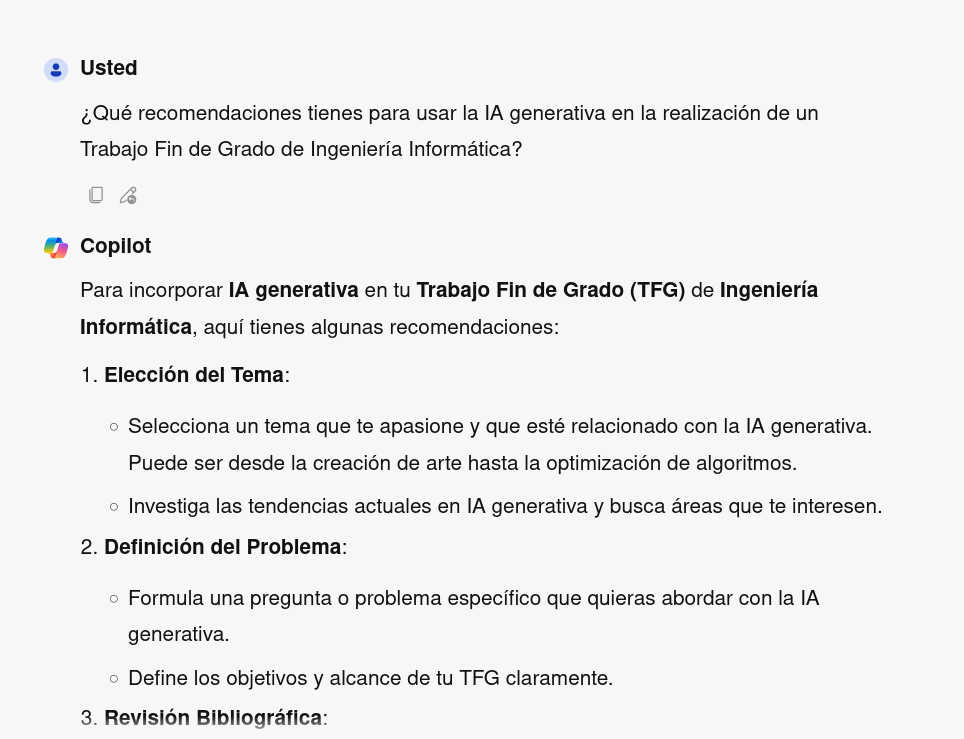
\includegraphics[scale=0.5]{images/Bing.png}
%    \caption{Respuesta (1/3) de Co-pilot de Bing ante la pregunta: ¿Qué recomendaciones tienes para usar la IA generativa en la realización de un Trabajo Fin de Grado de Ingeniería Informática? }
%    \label{fig:Bing}
%\end{figure} 

%\begin{figure}
%    \centering
%    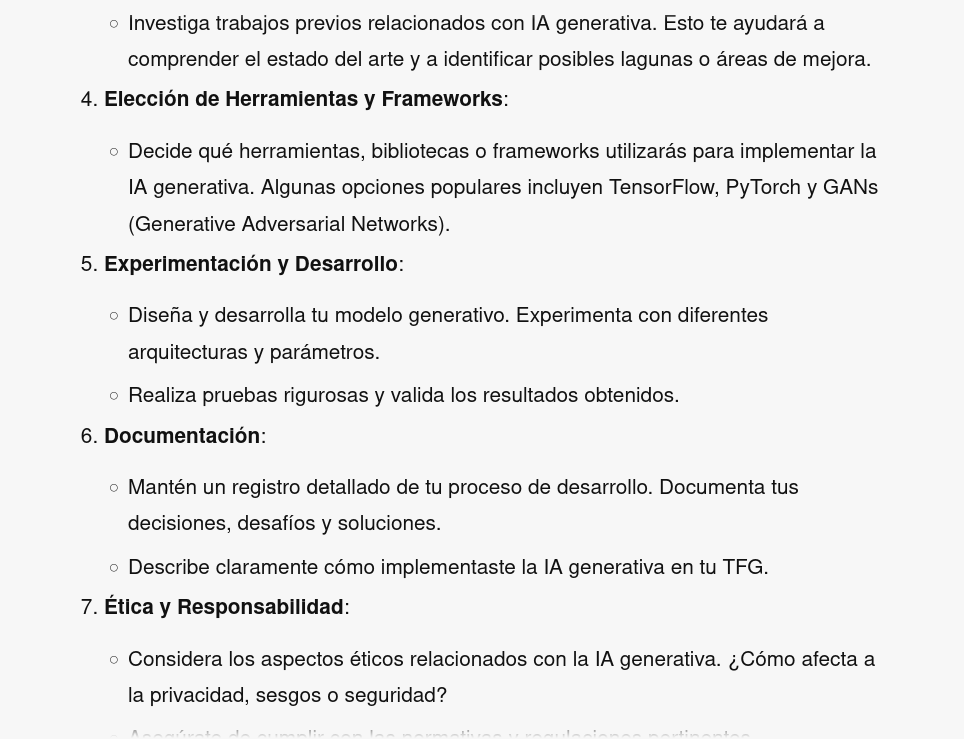
\includegraphics[scale=0.5]{images/Bing2.png}
%    \caption{Respuesta (2/3) de Co-pilot de Bing ante la pregunta: ¿Qué recomendaciones tienes para usar la IA generativa en la realización de un Trabajo Fin de Grado de Ingeniería Informática? }
%    \label{fig:Bing1}
%\end{figure} 

%\begin{figure}
%    \centering
%    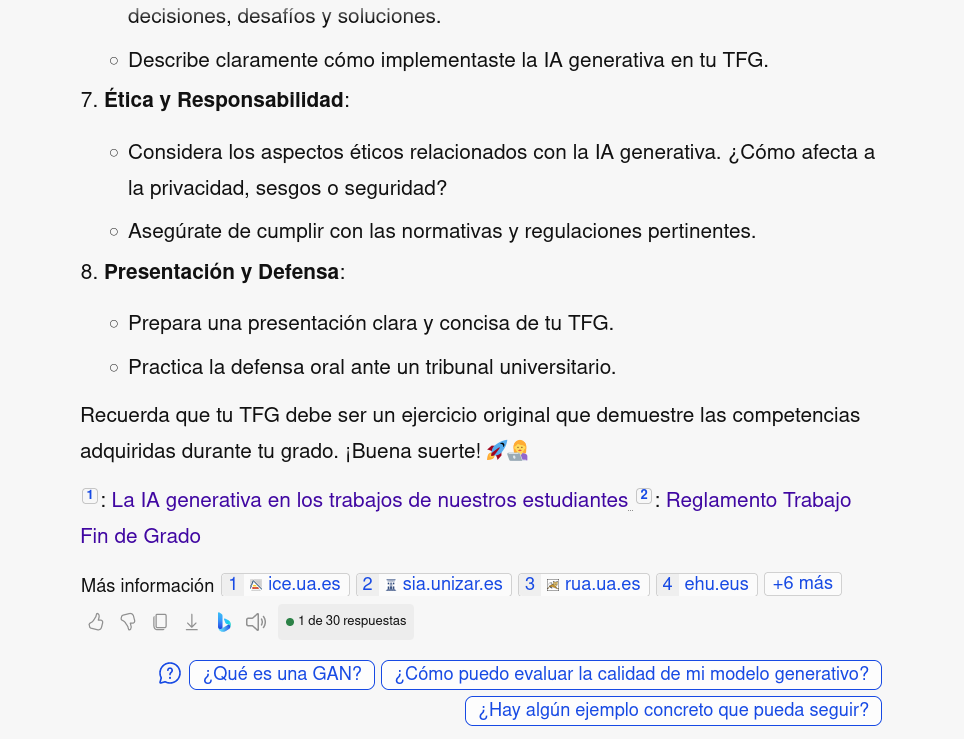
\includegraphics[scale=0.5]{images/Bing3.png}
%    \caption{Respuesta (3/3) de Co-pilot de Bing ante la pregunta: ¿Qué recomendaciones tienes para usar la IA generativa en la realización de un Trabajo Fin de Grado de Ingeniería Informática? }
%    \label{fig:Bing2}
%\end{figure} 

Como última recomendación, pregunta y revisa las directrices que indique tu Universidad, tu centro o tu coordinador del plan de estudios. 

Y recuerda que es tu TFG, apóyate en las IA generativas si lo consideras necesario pero el proyecto es un magnífico ejercicio de aprendizaje y entrenamiento que es bueno que lo hagas tú en su mayoría.


% Consejos sobre el proceso de desarrollo al estilo de lo que pone María José en sus diapositivas.
% Sobre el código (control de versiones, licencias…) (Aquí puedo ayudar yo (Pablo))
% Sobre cuestiones éticas de código y datos (Alberto).
% Qué cosas hacer y qué no hacer con ejemplos.


%%%%%%%%%%%%%%%%%%%%%%%%%%%%%%%%%%%%%%%%%%%%%%%%%%%%%%%%%%%%%%%%%%%%%%%%%%%%%%
%%%%%%%%%%%%%%%%%%%%%%%%%%%%%%%%%%%%%%%%%%%%%%%%%%%%%%%%%%%%%%%%%%%%%%%%%%%%%%
%Lo consensuado en la reunión del 21/02/24
%%%%%%%%%%%%%%%%%%%%%%%%%%%%%%%%%%%%%%%%%%%%%%%%%%%%%%%%%%%%%%%%%%%%%%%%%%%%%%
%%%%%%%%%%%%%%%%%%%%%%%%%%%%%%%%%%%%%%%%%%%%%%%%%%%%%%%%%%%%%%%%%%%%%%%%%%%%%%

%%%USAR https://docs.google.com/document/d/115O_20YW4Mjx1iJBBxxxDCDWJOBEL_rTzbeHVmI8Cak/edit#heading=h.n5bem9dnws3z



\chapter{La estructura general de la memoria}
\label{cap:EstructuraMemoria}
% [Autores: Pablo]
% Introducción general a cada una de las partes de la memoria.
% (este quizás sea de los últimos capítulos en escribir)
%Pablo revisa/copia/quita lo que vea oportuno de las recomendaciones generales -> Sobre la redacción de la memoria
% Lo siguiente añadido por María José

En este capítulo te mostramos de forma breve cómo estructurar la memoria de tu TFG. Esta estructura debería ser lo primero que deberías abordar, ya que te marcará un esquema mental del trabajo realizar y es muy importante que esté consensuada con la persona que te tutoriza. 

\section{Estructura general de un TFG/TFM}

La estructura depende del del tipo de TFG/TFM que realices (ver Apéndice \ref{cap:Tipologías}). En general, e independientemente del tipo de proyecto, todas las memorias deberían tener capítulos de \textit{Introducción}, \textit{Estado del Arte}, \textit{Conclusiones} y \textit{Bibliografía}. Aquí te damos una sugerencia de una posible organización de capítulos y secciones dentro de cada capítulo. 

\begin{enumerate}
    \item Introducción
        \begin{itemize}
            \item Contexto/Antecedentes
            \item Justificación/Motivación
            \item Objetivos/Hipótesis
            \item Estructura de la memoria
        \end{itemize}
    \item Estado del arte
        \begin{itemize}
            \item Descripción de dominio del problema
            \item Metodologías potenciales a aplicar
            \item Tecnologías potenciales para usar
            \item Trabajos relacionados
        \end{itemize}
    \item \textit{Distintos capítulos sobre la propuesta, que cubrirán:}
    \begin{itemize}
            \item Descripción de la propuesta
            \item Metodología
            \item Planificación temporal
            \item Presupuesto
            \item Otros capítulos y secciones según la metodología y tipo de proyecto
        \end{itemize}
    \item Conclusiones y trabajos futuros
    \begin{itemize}
            \item Conclusiones
            \item Trabajos Futuros
        \end{itemize}
    \item Bibliografía
    \item Anexos
\end{enumerate}

En el Capítulo \ref{cap:IntroducciónTFG} podrás ver en profundidad las descripciones de cada una de las secciones de la Introducción.


En el capítulo del Estado del Arte de tu trabajo se pueden incluir tantas secciones como se desee para agrupar bien los tipos de revisiones realizadas. Si la envergadura de estas secciones es muy grande, pueden incluso separarse en capítulos aparte, aunque te recomendamos que sólo ocupe uno. Tal y como se indica en el Capítulo \ref{cap:RevisionEstadoDelArte}, cada sección del estado del arte que se desee incluir deberá constar primero de una introducción explicando la metodología seguida para la revisión, luego la revisión concreta y al final unas conclusiones. %Es muy aconsejable incluir tablas con aspectos comparativos, ya que son más visuales y sirven de resumen. Por ejemplo, se recomienda incluir comparativas entre las potenciales tecnologías o metodologías, para luego en el capítulo de la propuesta justificar cuáles de ellas son las elegidas para la solución. También es común comparar los trabajos relacionados entre sí y según nuestros objetivos o requisitos.

Las secciones de los capítulos en los que desarrollamos nuestra propuesta están muy relacionadas con el tipo de proyecto y metodología. En las siguientes secciones de este capítulo te damos unas guías de cómo podría estructurarse según ello, aunque tienes información más detallada en el Anexo \ref{cap:Tipologías} para cada tipo de proyecto.

Finalmente, las dos secciones del capítulo de Conclusiones y Trabajo Futuro de tu TFG/TFM se explican con más detalle en el Capítulo \ref{cap:Conclusiones}.



\section{Proyectos de desarrollo}

Los proyectos de desarrollo suelen ser iterativos, y dependen de la metodología seguida (Ver Apéndice \ref{appendix:desarrollo}):

\subsection{Metodologías ágiles}

Cuando usamos una metodología ágil, como SCRUM, es buena idea crear la siguiente estructura de capítulos:
\begin{itemize}
    \item \textbf{Análisis}: incluimos planificación y presupuesto
    \item \textbf{Implementación}: Puede estar compuesto por las secciones:
    \begin{itemize}
                    \item \textit{Product Backlog}: listado de historias de usuario priorizadas y agrupadas en iteraciones o sprints
                    \item \textit{Iteraciones}: Una sección por cada iteración o \textit{sprint} describiendo las tareas y pruebas de cada iteración, e incluyendo gestión de riesgos si procede
                \end{itemize}
\end{itemize}
                

\subsection{Ciclo de vida clásico}
En este caso podemos crear un capítulo por cada una de las etapas.
                \begin{itemize}
                    \item \textbf{Análisis/Requisitos}: Requisitos funcionales y no funcionales, presupuesto, planificación, etc.
                    \item \textbf{Diseño}: Diagramas de clases, de secuencia, etc. Diseño de interfaces de usuario.
                    \item \textbf{Implementación}: Detalles concretos de la implementación de cada componente.
                    \item \textbf{Pruebas}: Descripción de las pruebas unitarias, de integración, etc.
                \end{itemize}
\subsection{Otros ciclos de desarrollo}
Si usamos otro tipo de desarrollo deberemos adaptar los capítulos a sus etapas.


\section{Proyectos de investigación}
Los proyectos de investigación tienen su propia estructura (Ver Apéndice \ref{appendix:investigacion}), en la que se le da especial importancia a la discusión de los resultados. 

Para empezar en un proyecto de investigación, la introducción también debería contar con las siguientes secciones:
    \begin{itemize}
                \item \textbf{Preguntas de investigación}: identificación de problemas o carencias que se van a abordar en el proyecto 
                \item \textbf{Hipótesis}: enunciados a demostrar o probar (suele ser uno de los objetivos el demostrar una hipótesis concreta)
                
    \end{itemize}

%\item \textbf{Evaluación de las hipótesis}: Elección de un método de investigación, determinación de experimentaciones a realizar, elección de instrumentos de recogida de datos y de herramientas análisis de datos y de evaluación.
El resto de capítulos (además de la Introducción, Estado del Arte y Conclusiones, claro) puede ser el siguiente:
\begin{itemize}
    \item \textbf{Metodología}: Explicación de los pasos a seguir, algoritmos a implementar, ecuaciones, variables a medir, etc.
    \item \textbf{Experimentos}: definir los parámetros exactos que se van a utilizar y explicaciones más específicas sobre los experimentos a realizar.
    \item \textbf{Resultados}: Variables y valores obtenidos. Tablas de análisis, matrices de correlación, etc.
    \item \textbf{Discusión}: Interpretación de resultados, referenciando estado del arte e hipótesis u objetivos.
\end{itemize}
    
Si alguno de estos capítulos se te queda corto se puede combinar con otro: por ejemplo, ``Metodología Experimental'' o ``Resultados y discusión''.
        
\section{Proyectos de revisión de estado del arte} 

En este tipo de proyectos (Ver Apéndice  \ref{appendix:revisionestado}) la mayor envergadura la tendrá el capítulo (o capítulos) del estado del arte. Sin embargo, justo después de la \textit{Introducción} deberías incluir un capítulo llamado \textit{``Metodología''}, donde expliques el proceso seguido para la revisión (Dónde buscar, qué palabras clave utilizar, cómo filtrar la búsqueda, qué características revisar/comparar, etc.).


\section{Conclusión}


 Las metodologías de proyectos no son exclusivas entre sí, por ejemplo, un proyecto de tipo desarrollo podría incluir una parte de validación que implique aplicar la metodología de investigación. Igualmente, un proyecto de investigación puede necesitar del desarrollo de software. Por ello, se pueden añadir secciones de un tipo en otro tipo.

En resumen, la estructura no está escrita en piedra y puede variar dependiendo de lo que vayas a hacer. Por eso es muy importante consensuarla con tu director/a y también tener en cuenta que puede cambiar durante el desarrollo del proyecto. En los siguientes capítulos de este libro te explicamos con más detalle cada uno de los capítulos y secciones de la memoria de tu proyecto.


\chapter{La introducción del TFG}
\label{cap:IntroducciónTFG}

\section{Introducción}

En este capítulo nos centramos en describir las pautas para redactar el capítulo de introducción, que normalmente será el primero de la memoria y que también será el contenga cierta entidad dentro de la misma, pues es vital para que el lector entienda de qué trata tu TFG.

En síntesis, el capítulo de introducción debe destinarse a ofrecer una panorámica general del trabajo llevado a cabo, sobre todo en lo referente al contexto y razones que lo han motivado, de forma que se acerque al lector a los temas tratados en el mismo. Como veremos más adelante, esto ocupará dos secciones específicas del capítulo.

Por otro lado, como con cualquier otra sección de la memoria, tener presente el punto de vista del lector y facilitarle su comprensión resulta especialmente relevante. Ello fomentará que se anime a profundizar y seguir leyendo el resto de secciones. Si además se trata de alguien interesado en trabajar en líneas iguales o parecidas, se le motivará a que pueda consultar el resto del trabajo y continuarlo en el punto en el que se dejó en la memoria, o lo revise y hasta mejore.

Finalmente, desde un punto de vista pragmático, hemos de tener en cuenta que, por el mero hecho de enviar el TFG para someterlo a su defensa pública, ya tenemos un conjunto de lectores asegurado que, además, van a leer y consultar la memoria elaborada desde un punto de vista crítico. En efecto, dichos lectores serán las personas que formen parte del tribunal de evaluación del TFG, o al menos, el tutor o tutores, según venga establecido en la guía docente correspondiente.

Si el trabajo lo evalúa un tribunal, es muy probable que alguna o todas las personas que lo formen, no estén tan familiarizados como tú en el tema del trabajo, o no sepan por qué es importante o pertinente trabajar en el mismo. Es posible incluso que para alguno sea la primera vez que lee algo acerca de las temáticas principales del TFG. El capítulo de introducción sirve para aclarar todos estos aspectos y ayudar al tribunal a comprender el problema entre manos y valorar mejor las contribuciones del trabajo.

Por esto mismo, siendo el primer capítulo de la memoria, es uno de en los que conviene poner especial cuidado y esmero en la redacción, de forma que sea especialmente ágil, concisa y clara. También es importante seguir cierto orden y estructura a la hora de presentar (\textit{introducir}) los contenidos, siguiendo un patrón que atienda al \textit{Qué}, para describir el contexto); \textit{por qué}, para dar razón o motivar el trabajo, y \textit{por tanto}, para definir objetivos consecuentes con la motivación y el contexto del trabajo.

Podría ocurrirnos que aun tratando de ser breves, nos cueste ajustarnos a esta forma de estructurar, bien porque no encontremos muchas cosas que decir (mucho contexto), o porque de forma natural queramos conectar enseguida el contexto con la motivación. También, como se trata del primer capítulo y no estamos acostumbrados a documentar trabajos tan extensos, experimentemos cierto bloqueo a la hora de escribir. Esto mismo es lo que nos han reportado estudiantes como vosotros en un estudio previo \colorbox{yellow}{[REFERENCIAR ENCUESTAS]}. Como con el resto de secciones de la memoria del TFG, en las siguientes secciones daremos algunas pautas o pistas, con ejemplos, sobre cómo abordar o con qué tipo de contenidos completar el capítulo de Introducción. De forma similar a lo que ocurre con el primer capítulo de una serie de televisión o un libro cualquiera, el capítulo de introducción del TFG debe servir para conectar y enganchar con el lector, atrayendo su atención y provocando su curiosidad por el trabajo. De hecho, las productoras de televisión suelen invertir cantidades de dinero por minuto de metraje en los primeros minutos o el tráiler de una producción muy superiores a las que invierten en otros minutos de capítulos ordinarios. Saben que ese primer contacto con el espectador es fundamental para despertar su interés.

Seguramente hayas experimentado una situación similar al comenzar a leer otros libros o incluso otras memorias de TFG: si encuentras las primeras páginas difíciles de entender o pesadas, es más fácil abandonar la lectura de las siguientes o pasar por alto detalles relevantes, ya que cuesta más mantener la atención por el sobreesfuerzo requerido. Ponte especialmente en el lugar de tus potenciales lectores cuando escribas este capítulo. Como dice el refrán, \textit{para la primera impresión no hay una segunda oportunidad}.

Ten en cuenta también que este primer capítulo, junto con el de las conclusiones, será también uno de en los que en más se fijen quienes evalúen el trabajo. Esto se debe, por un lado, a que se encuentra al principio de la memoria, y lógicamente aparece y se lee antes; y por otro lado, a que en este capítulo deben reflejarse en una sección separada los objetivos del TFG. Por tanto, lo normal será que quien lo evalúe, acuda con frecuencia a dicha sección de objetivos y la contraste con las aportaciones reflejadas en la memoria, las conclusiones del trabajo y lo que se presente durante la defensa. 

Por último, este capítulo no deberá ser muy extenso (con 5 o 6 páginas puede ser más que suficiente), ya que se trata simplemente de dar un anticipo de la información que se detallará más adelante en el resto de secciones de la memoria para quien esté realmente interesado en el trabajo. Lo que sí es importante es tratar de respetar la estructura del capítulo, ya que suele ser bastante universal. Es decir, una especie de estándar o protocolo relativo a la forma de estructurar un libro, que en este caso es la memoria del TFG. Como ocurre con los estándares o los protocolos, quienes se adhieren a ellos, se obligan a respetar una serie de formatos y estructuras para que sea posible la comunicación o interacción entre diferentes actores. Análogamente, respetar una misma estructura de documento, en este caso, la memoria de un TFG, y un mismo tipo de contenidos en cada una de ellas, hará que tutores y revisores experimentados puedan recorrer y consultar la memoria de forma más eficaz, ya que podrán encontrar el tipo de información que buscan en las secciones previstas para ello.

Por la importancia de este capítulo, a veces se redacta al final del todo, cuando el resto de la memoria ha sido completada. La ventaja de esta aproximación es que ya tienes una visión global de tu TFG y su memoria, lo que posibilita que puedas centrarte en este capítulo y ser capaz de plasmar la esencia del TFG mucho mejor.

A continuación pasaremos a presentar las secciones, junto con sus contenidos y pequeños ejemplos de los mismos, que deben aparecer en el capítulo de introducción de un TFG. Normalmente, dichas secciones serán las siguientes: contexto, motivación, objetivos del TFG y estructura de la memoria.

% [Autores: Manolo]
\section{Contexto}\label{Contexto}
Esta sección está destinada a responder a la pregunta "¿Qué?". Qué existe, qué es o en qué consiste, qué se puede hacer, cuál es el tema de estudio o del trabajo, en qué dominio se sitúa, cómo se viene abordando una determinada actividad (es decir, de qué forma, qué enfoques, propuestas o aproximaciones se vienen defendiendo), qué propiedades, qué mercado, qué permite, etc., son ejemplos de cuestiones que debemos responder a la hora de presentar el contenido de esta sección. Dejamos por aquí algunas pistas o sugerencias de contenidos de que deben aparecer.

\subsection{Qué de qué. Definiciones}

En conjunto, la respuesta a los diferentes \textit{"qués"}, nos dará como resultado el contexto del trabajo y orientarán al lector con respecto al contenido de la memoria. Por ejemplo, si nuestro TFG se encuadra en el ámbito de los \textit{asistentes inteligentes}, una buena forma de comenzar a escribir el contexto es decir qué es un \textit{asistente inteligente} o qué tipo de sistemas software o hardware vamos a entender por tales.

Esto es especialmente importante cuando un mismo término se use de forma diferente en varios contextos. Para ello, es bueno comenzar con una definición o introducir alguna frase aclaratoria del tipo \textit{"... Si bien existen diferentes acepciones para el término} \textless término\textgreater, \textit{en este trabajo vamos a entender por tales aquellos que..."}. Lo mismo también es aplicable cuando nos vayamos a referir con diferentes términos a una misma idea o concepto. Por ejemplo, siguiendo con el caso de los asistentes inteligentes, si nos vamos a referir a ellos también como \textit{sistemas conversacionales}, podemos incluir una frase aclaratoria del tipo \textit{...Es frecuente encontrar referencias a los asistentes inteligentes denominándolos } sistemas conversacionales. \textit{En esta memoria utilizaremos indistintamente ambos términos para referirnos a aquellos sistemas que...}.

También podemos explicar brevemente la diferencia entre términos, para demostrar que hemos tomado la decisión conscientes de la existencia de matices, pero que no son relevantes en el contexto de nuestro TFG. Por ejemplo, si nuestro trabajo se enmarca en el ámbito \textit{Ubitquitous Computing} (Computación Ubicua) y nos vamos referir a estos sistemas también como del ámbito del \textit{Pervasive Computing}, podríamos decir \textit{``...En Computación Ubicua, el objetivo principal es proporcionar a los usuarios la capacidad de acceder a servicios y recursos en todo momento e independientemente de su ubicación, mientras que en Pervasive Computing, el objetivo principal es proporcionar servicios emergentes y espontáneos creados sobre la marcha por dispositivos móviles que interactúan mediante conexiones ad hoc. Existiendo esta diferencia, la realidad es que en muchas situaciones, ambos paradigmas de computación ofrecen las mismas soluciones y podemos referirnos a ellas como formas de Computación Ubicua o Pervasive Computing, indistintamente...''}.

\subsection{No despistes al lector}
Por otro lado, debemos tratar de seguir un enfoque bastante sintético, tratando de ir directamente al grano, sin digresiones sobre temas (otros "qué") que  se alejen del núcleo del trabajo. En efecto, es muy importante evitar incluir información o hacer referencia a cuestiones que no se hayan abordado con cierta profundidad, ya que pueden despertar falsas expectativas en el lector acerca de lo que va a encontrar. Como ya hemos comentado, conviene ponernos en el lugar de quien va a leer la memoria. Pensemos en nuestra propia experiencia como lectores de otros libros o manuales técnicos (una memoria de TFG es en parte eso). Si cuando consultamos el índice, la sinopsis de la contraportada o la introducción se nos hablaba de una tecnología, y por esto mismo nos animamos a sacar el libro de la biblioteca, y luego esta se usaba de una forma muy marginal en el resto del documento, nos sentimos decepcionados y que hemos perdido el tiempo.

Así, imaginemos la siguiente situación. En nuestro proyecto o desarrollo hemos utilizado unas técnicas bastantes complejas de aprender y con una curva de aprendizaje bastante plana al comienzo, siendo esta una dificultad conocida de dichas técnicas. A pesar de ello, hemos conseguido dominarla y resolver un problema concreto e interesante. Sin embargo, en nuestro trabajo no hemos realizado ninguna aportación que facilite el uso de dichas técnicas. En este caso, tendríamos que evitar hacer una referencia reiterada a la dificultad de manejar dichas técnicas, ya que el lector o revisor podría esperar que el trabajo terminará abordando ese problema, debido a que  se menciona varias veces y parece importante.

Esto ocurre con frecuencia con problemas conocidos: ruido en los datos en los mismos \textit{outliers}, usabilidad de una aplicación, rendimiento de un algoritmo, consumo energético, etc. Estos problemas podrían ser desafíos vigentes de la tecnología que utilicemos en nuestro TFG, pero si no hemos realizado ninguna aportación para paliarlos, lo mejor es no mencionarlos más de una vez en nuestro capítulo de introducción. Así, si decimos que en ciertos tipos de conjuntos de datos existe mucho ruido, que actualmente se está trabajando en técnicas que al generarlos reduzcan dicho ruido y que una línea de trabajo interesante en relación con esos conjuntos de datos es la eliminación del ruido, será porque en nuestro TFG, el ruido y su gestión se habrán abordado de alguna forma novedosa. Si, por el contrario, pero en nuestro TFG no hemos hecho o aportado ninguna solución para gestión del ruido, estaremos creando cierta confusión en la persona que lea el trabajo.

La experiencia con muchos trabajos que hemos supervisado o evaluado en tribunales de defensa en el pasado nos enseña que buenos trabajos de fin de grado se ven penalizados o deslucidos por referencias a aspectos o cuestiones en las memorias, que no eran el objeto o contribución nuclear del trabajo.

%\subsection{Respeta la estructura}
%Por último, indicar que una tendencia habitual al presentar una tecnología, un estado de la cuestión sobre algún tema, describir un dominio de aplicación, etc., es comentar a la vez los problemas o deficiencias con los que vengan aparejados. Por ejemplo, podemos haber realizado un TFG sobre un sistema de monitorización de la actividad física que sincroniza datos que recibe de sensores colocados en el cuerpo y graba en vídeo sesiones de entrenamiento. Hasta aquí habríamos descrito un \textit{qué}, es decir, monitorizamos la actividad física sincronizando vídeo y datos de sensores. Nuestro sistema es novedoso porque hasta la fecha no se dispone en el mercado de soluciones de bajo coste o abiertas que satisfagan dicha funcionalidad. En este caso, una tentación frecuente es conectar ambas ideas con una descripción como la siguiente: \textit{En los últimos años se han popularizado los sistemas y plataformas de monitorización remota de la actividad física a través de sensores corporales para estudiar el rendimiento durante el ejercicio físico. Estos estudios pueden complementarse con el análisis de vídeos o grabaciones de los sujetos mientras realizaban la actividad física registrada con dichos sensores} (hasta aquí un \textit{qué}).\textit{Sin embargo, no existen abundan soluciones de bajo coste que, de forma integrada, permitan gestionar la información obtenida desde ambos tipos de fuentes, es decir, vídeo y datos de sensores...} (habríamos comenzado a describir una \textit{deficiencia} o a dar un motivo, es decir, responder a \textit{por qué} hemos realizado el trabajo que se presenta.

%La conexión de ambas ideas en el resumen sería razonable, ya que por limitaciones de espacio, no habría opción a otras alternativas. En cambio, en el caso de la Introducción conviene cierta disciplina y estructura a la hora de presentar los contenidos. Como veremos en la siguiente sección, las razones que justifican la pertinencia del trabajo desarrollado deben describirse en la siguiente sección de \textit{motivación}.

\subsection{Estructura del introducción: algunas sugerencias}
A lo largo de toda la memoria, es esencial respetar la estructura del documento. Debemos respetar que tras un \textit{¿Qué} debe aparecer un \textit{porqué}.
Si encontramos dificultades para ajustarnos la estructura presentada porque necesitemos dar enseguida argumentos o motivaciones para el trabajo (que vendrán en la siguiente sección \ref{Motivation}, pensando que nos queda demasiado pobre si no lo hacemos, o no sabemos qué más comentar acerca de lo que ya existe, podemos completar proporcionando breves datos acerca de cuestiones como usuarios actuales o potenciales beneficiarios de una tecnología, orígenes de la misma, tamaño de mercado o volumen de facturación, iniciativas políticas, legislación, etc. Por ejemplo, si nuestro TFG versa sobre una plataforma para la promoción de hábitos nutricionales saludables en población infantil, para describir el contexto podemos apoyarnos de datos como \textit{"Un estudio reciente llevado a cabo en el ámbito del programa conocido como Estrategia de Promoción de una Vida Saludable en Andalucía (2024-2030), dependiente de la Consejería de Salud y Consumo de la misma comunidad, estima que la prevalencia del exceso de peso en la población infantil (de 2 a 17 años) andaluza se sitúa en el 33,40\%, situándose de desde el comienzo de estos estudios en varios puntos por encima de la media nacional"}\footnote{https://www.juntadeandalucia.es/organismos/saludyconsumo/areas/planificacion/estrategia-promocion-vida-saludable-andalucia.html}. Como vemos en este texto de ejemplo, hemos aprovechado para explicar indirectamente qué vamos a entender por población infantil (la que se encuentra entre 2 y 17 años de edad). Asimismo, hemos proporcionado también una referencia para demostrar que nos hemos documentado y acudido a fuentes oficiales para proporcionar el contexto de nuestro trabajo. En el capítulo  \ref{bibliografia} Bibliografía profundizaremos más en cómo citar los distintos trabajos.

Por último, si nos ocurre lo contrario, es decir, que tenemos exceso de contenidos con los que documentar el contexto del trabajo, trataremos de ser breves, describiendo o reservando los detalles para el capítulo de revisión del estado de la cuestión. Recordemos que en este capítulo hemos de tratar de ser concisos y presentar la información de forma atractiva para facilitar al lector la revisión de contenidos posteriores, además de despertar su curiosidad por leer el resto de la memoria.

\section{Motivación}\label{Motivation}
Esta sección debe justificar la razón de ser del trabajo realizado. Si la primera sección \ref{Contexto} Contexto, buscaba responder a la pregunta \textit{"Qué"}, esta sección debe más bien tratar de responder a preguntas como \textit{qué falta}, \textit{qué necesidades existen}, \textit{qué problemas tiene} o \textit{cómo se puede potenciar}, aquello que presentamos en dicha sección de contexto. Si, por ejemplo, nuestro trabajo trata sobre el análisis de la facilidad de navegación de un sitio web y conocemos una tecnología o una técnica que pensamos que podría aplicarse para monitorizar las distintas páginas que visitan los usuarios, pero que aún nadie la ha probado, podemos justificar nuestro trabajo indicando que el uso de dicha tecnología o técnica aún no se ha explorado para el análisis de la usabilidad de un sitio web. Como es plausible que su aplicación facilite dicha tarea, queda justificado hacer un TFG que lo investigue. La misma argumentación puede seguirse cuando describimos problemas, carencias, o funcionalidades por desarrollar y que decidimos abordar en nuestro TFG.

Por otro lado, si nuestro TFG ha consistido en la simulación de un encargo profesional relacionado con nuestro grado, es interesante indicar \textit{qué competencias} hemos adquirido o mejorado al realizar el mismo.

Se trata, de justificar por qué hemos llegado hasta aquí, o por qué es bueno o conveniente trabajar de la manera y en el ámbito que lo hemos hecho. En definitiva, hay que responder a la pregunta \textit{"Por qué"}: porque faltaba una determinada funcionalidad que hemos desarrollado; porque no se ha explorado la aplicación de una técnica en un determinado ámbito y podemos demostrar que se pueden obtener resultados interesantes haciéndolo; porque atendiendo una determinada necesidad se mejora la vida de ciertas personas; porque aplicando algo de distinta manera se obtienen mejores resultados que los que se vienen obteniendo en un determinado ámbito, etc.

Así, dependiendo del trabajo, podremos presentar unas motivaciones u otras, pero no debe resultarnos difícil encontrar un buen puñado de ellas. Algunos ejemplos podrían ser: 

\begin{itemize}
  \item Atención a un determinado colectivo en relación a una tecnología. Por ejemplo, nuestro trabajo podría consistir en el diseño de unas etiquetas en Braille y una aplicación para un dispositivo móvil capaz de interpretarlas para colocarlas junto a las obras de arte de un museo de forma que las personas con discapacidad visual puedan localizarlas y acceder a información enlazada que les proporcione información acerca de dichas obras. Nuestro TFG viene justificado o motivado por la necesidad de atender a ciertas personas y la ausencia de algo parecido.
  \item Problemas de usabilidad. Por ejemplo, los dispositivos para interactuar con agentes conversacionales inteligentes a veces tienen dificultades para captar correctamente las intenciones de sus usuarios, sin embargo tampoco existen métodos o herramientas para facilitar el análisis de por qué la interacción falla y nuestro trabajo ha consistido en desarrollar un sistema que demuestra que haciendo uso de una determinada tecnología es posible depurar las interacciones con dichos sistemas.
  \item Ausencia de una funcionalidad específica que demande un determinado tipo de usuarios o colectivo sobre ciertos conjuntos de datos. Por ejemplo, sabemos de las plataformas de compartición y reproducción de música bajo demanda. Algunas de estas ofrecen APIs (\textit{Application Programming Interface}) que ofrecen datos generalistas sobre artistas y descargas adaptadas a sus consumidores (este sería el \textit{qué}), pero conocemos que dentro del colectivo de los propios músicos o creadores de contenidos, estarían más interesados en disponer de herramientas que ofrecieran un análisis más pormenorizado de sus obras y evolución en ciertos períodos. Entonces, decidimos hacer un TFG para cubrir esta carencia desarrollando las funcionalidades pertinentes.
  \item Si nuestro trabajo va a consistir en ejecutar un encargo profesional\footnote{Que podrá ser simulado o real.}, como por ejemplo, el desarrollo de un sistema de información para la gestión de un gimnasio, podremos enumerar distintas competencias o habilidades que queramos adquirir y/o reforzar. De hecho, su adquisición ya representa por sí misma una motivación o justifica el desarrollo del TFG.
\end{itemize}

Por otro lado, como con todas las secciones de la memoria, debemos mantener el hilo y presentar un relato coherente. Por tanto, Como vemos, en esta sección concretamos un poco más el ámbito en el que hemos trabajado (para los trabajos más aplicados o que simulen encargos profesionales) o donde hemos aportado algo novedoso (para aquellos trabajos con alguna componente de investigación o innovación), en línea con la idea de centrar el tema del trabajo y no divergir o distraer a los potenciales lectores de la memoria.

\section{Objetivos del TFG}
A partir de los \textit{"qué"} y los \textit{"por qué"}, esto es, del contexto y motivación de las dos secciones anteriores, la sección de objetivos debe representar un \textit{"por tanto", "en consecuencia"} de lo que ya se ha explicado. Por ejemplo, como falta esta funcionalidad en este ámbito o dominio particular, nos proponemos abordar un desarrollo que cubra dicho vacío, o bien, como cierta tecnología presenta los problemas que ya se han descrito, proponemos un objetivo que resuelva o mitigue dichos problemas. Como venimos insistiendo, alinear los objetivos con el contexto y la motivación del trabajo, también ayudará a revisar mejor el trabajo y no distraer al lector.

Lo normal será también que los objetivos se presenten describiendo en primer lugar un objetivo principal\footnote{También podemos denominarlo como objetivo general (OG).} que sea lo más comprensivo posible, de forma que englobe las tareas o resultados más destacables de nuestro TFG y,  a continuación, una serie de objetivos más particulares o concretos, también denominados como específicos, sobre resultados o tareas más sencillas. Esto demostrará que hemos analizado el problema a abordar y que hemos sido capaces de descomponer y estructurar una tarea compleja en otras más sencillas para conseguir un alcance mayor. Como siempre, pero especialmente en esta sección, conviene que nos expresemos con concisión. Así, una buena frase para comenzar esta sección puede ser:

\textit{El objetivo principal de este TFG es } \textless nuestro principal objetivo\textgreater. \textit{Este objetivo principal se ha articulado en torno a la consecución de los siguientes objetivos específicos}:
\begin{itemize}
  \item \textit{Objetivo específico 1}
  \item \textit{Otro objetivo específico}
  \item \textit{Y otro más}
  \item \textit{...}
\end{itemize}

Como pista, podríamos decir que el objetivo principal debería ir alineado con el título del proyecto, para dotar de coherencia a la memoria. Asimismo, en la lista o enumeración anterior de objetivos específicos, deberán aparecer primero aquellos que sirvan de base o deban alcanzarse antes de abordar otros, secuenciando los pasos que deben darse para alcanzar gradualmente el objetivo principal.

Cabe indicar en este punto que los objetivos deben estar formulados en infinitivo: estudiar, analizar, desarrollar, comparar, evaluar, etc.  

Por otro lado, las características principales que debemos buscar al fijar (y expresar) los distintos objetivos en el contexto de un proyecto, en general, y de un TFG en particular, es que sean realistas y concretos. Sin ánimo de seguirlas exhaustivamente, podemos guiarnos por las orientaciones del marco de trabajo SMART \cite{doran1981there}, en particular, las revisiones más modernas y orientadas a proyectos tecnológicos, como las que podemos encontrar en el sitio web de \href{https://www.atlassian.com/blog/productivity/how-to-write-smart-goals}{Atlassian}. SMART es el acrónimo de \textit{Specific}, \textit{Measurable}, \textit{Achievable}, \textit{Relevant}, y \textit{Time-Bound}, es decir, los objetivos que fijemos deben abordar un área concreta de trabajo o mejora (esto es, ser \textit{específicos}); incluir alguna métrica o valor objetivo para seguir y evaluar su grado de progreso o cumplimiento (para que sean \textit{medibles}); es factible (realista) conseguirlos (es decir, son \textit{alcanzables}); son pertinentes o necesarios para el TFG (por tanto, \textit{relevantes}); y finalmente, puede anticiparse un plazo de tiempo para su ejecución (es decir, son \textit{planificables} o acotarse en el tiempo).

Finalmente, indicar que, aunque idealmente los objetivos de un trabajo se establecen (al menos informalmente) al comienzo del mismo y se van abordando conforme a una determinada planificación, la realidad y el posible desconocimiento de algunas tecnologías que estemos utilizando, nos lleven a modificar nuestros planes iniciales y revisar dichos objetivos, bien porque vemos más interesante algunas posibilidades que hemos descubierto, o bien porque nos encontramos con algún imprevisto que nos impida alcanzarlos.

Por ello, desde un punto de vista estratégico y siendo también realistas, podemos dejar para el momento de finalización de la memoria la redacción concreta de los objetivos, según el trabajo que ya conoceremos con seguridad que hemos completado. La mayoría de las veces infravaloramos el tiempo que vamos a necesitar para realizar una tarea y sobrestimamos nuestras capacidades, pero digamos que no hace falta que lo explicitemos en nuestra memoria. Al fin y al cabo, ordinariamente tendremos que hacer una \textit{defensa} del mismo, y si indicáramos posteriormente que no hemos alcanzado los objetivos que nos fijamos, además de resultar extraño, nos estaríamos despojando de argumentos para defender o justificar nuestra capacidad de análisis o planificación.  

También indicar que se suelen poner, además de los objetivos del proyecto, algunos objetivos personales que se desean alcanzar con la elaboración del mismo. Estas metas reflejan ciertos aprendizajes o puesta en práctica de metodologías o tecnologías que, aprovechado que estás haciendo el TFG quieres conseguir. Un par de ejemplos podrían ser "aprender y aplicar en un proyecto real la metodología SCRUM" o "aprender el \textit{framework} Django y ponerlo en práctica en un proyecto real". 

\section{Estructura de la memoria}
Esta sección está destinada a comentar cómo hemos organizado el resto de la memoria, por lo que simplemente debemos describir qué bloques principales o capítulos hemos utilizado y, en una frase o dos, dar una breve idea de qué contiene cada uno. La idea es mostrar cómo queda estructurado el texto y qué se va a describir en cada una de las partes del mismo.

Desde un punto de vista visual, podríamos utilizar una enumeración en forma de lista de elementos separados por puntos.

Por ejemplo, podríamos escribir algo como: \textit{"En el capítulo 1 se han presentado el contexto y motivación de este trabajo, así como los principales objetivos que nos hemos propuesto para abordar la problemática asociada a \textless X\textgreater. El resto de la memoria se ha estructurado como sigue:}

\begin{itemize}
  \item \textit{En el capítulo 2 se describe el estado de la cuestión en relación a las principales tecnologías/métodos/técnicas/estudios} (escribir lo que corresponda)\textit{ sobre \textless lo-que-hayamos-usado-en-nuestro-TFG \textgreater}.
  \item \textit{En el capítulo 3 se presenta la propuesta que hemos realizada para} \textless abordar-el-problema-u-objeto-principal-de-nuestro-TFG \textgreater.
  \item \textit{El capítulo 4 contiene la especificación y arquitectura de los principales módulos/interfaces/servicios que hemos desarrollado}.
  \item ...
  \item \textit{En el último capítulo se presentan las conclusiones y trabajos futuros a partir del presente TFG}.
  \item \textit{Finalmente se presentan las referencias bibliográficas usadas en este trabajo}.
\end{itemize}

Como es lógico, lo más práctico será escribir esta sección cuando hayamos completado todos los demás capítulos y conozcamos la estructura definitiva que vamos a dar a la memoria de TFG.

\chapter{La revisión del estado del arte} \label{cap:RevisionEstadoDelArte}

% [Autores: Pablo, Juanma]

\section{Introducción}
¿Qué es una revisión el estado del arte? Básicamente un análisis del conocimiento actual sobre un tema de tal forma que te permite identificar qué hay hecho sobre el mismo (qué se ha investigado o desarrollado -- visión general del conocimiento) y qué lagunas existen. Es el paso previo para que tú puedas realizar una propuesta que mejore lo que hay ya hecho y, sobre todo, que sitúes tú trabajo en un contexto. La idea es que busques recursos bibliográficos (fundamentalmente literatura relevante en forma de artículos científicos) y los estudies, comprendiendo el problema y las soluciones propuestas para resolverlo, entendiendo los métodos aplicados y que, como consecuencia de ese estudio, seas capaz de tener una imagen general y clara del tema y de su evolución e identifiques situaciones o elementos de mejora. En lo que se refiere al TFG no es resumir los recursos que has encontrado, sino analizarlos, sintetizarlos, clasificarlos, contextualizarlos y evaluarlos de forma crítica para obtener una imagen clara del estado del conocimiento.

Por tanto, ¿para qué te sirve realizar una revisión del estado del arte en tu TFG? Es una de las primeras tareas que tienes que llevar a cabo una vez asignado el TFG ya que te permitirá inicialmente familiarizarte con el problema y con todo lo que se ha hecho en el campo de tu TFG. Y también de forma práctica, como se aborda en una fase inicial, para evitar que hagas algo que ya está hecho. También sirve para que identifiques lagunas o brechas en el conocimiento o problemas no resueltos donde tu TFG puede aportar. El que la memoria de tu TFG conste de una buena sección del estado del arte es importante ya que está demostrando que conoces lo que hay hecho en el contexto de tu TFG y también muestra tu capacidad de síntesis y análisis. Además, te va a permitir desarrollar un marco teórico y metodológico para tu proyecto y posicionarte con respecto a las metodologías, teorías o desarrollos existentes, con objeto de diferenciar tu trabajo. 

Veamos un par de ejemplos. En el primero, tienes entre mano un TFG en el que deseas aplicar inteligencia artificial a la gestión de invernaderos. Lo primero que tienes que hacer, por tanto, es preguntarte qué se ha hecho en este campo, qué problemas se han abordado, qué técnicas se han aplicado, qué resultados se han obtenido. Y esto sólo puedes hacerlo haciendo una búsqueda bibliográfica, leyendo todos los recursos que obtengas y analizándolos. De esta forma puedes darte cuenta que el campo en general está muy trillado, pues es algo donde se ha trabajado mucho, se han producido muchas aportaciones y con buenos resultados, y quizá que tu aportación sería insignificante o poco relevante. Pero con este análisis, además de llegar a conocer bien el tema y de ser capaz de describir cuáles han sido sus avances, te has dado cuenta que en el área del riego inteligente por goteo los métodos que se ha aplicado no funcionan del todo bien y no se adaptan correctamente a las circunstancias específicas de los invernaderos (fundamentalmente por los diferentes tipos de suelo, de plantaciones y condiciones ambientales, por ejemplo). En este caso acabas de detectar una posible línea de trabajo y, por tanto, un lugar por donde poder orientar tu TFG y realizar una aportación metodológica o práctica: la aplicación de algoritmos genéticos a la gestión eficiente del riego (por decir algo).

Imagina una segunda situación en la que vas a desarrollar una aplicación móvil para ayudar a las personas mayores en caso de necesidad. ¿Qué otras aplicaciones hay en el mercado que estén en este ámbito? En este caso, los recursos bibliográficos no sólo serán artículos científicos donde se presentan esas aplicaciones y se evalúan, sino también  sitios web de aplicaciones de este estilo, en la que cuentan sus prestaciones y funcionalidades. En este caso debes hacer una búsqueda exhaustiva y obtener todas las aplicaciones, analizar su funcionamiento en el caso de que te las puedas descargar y probar, o estudiar las prestaciones publicadas y clasificarlas por funcionalidades. Así conocerás qué hace la ``competencia'' y qué puntos fuertes y débiles tiene cada una. Con esta información establecerás las prestaciones que tendrá que tener tu aplicación (las habituales que todas tienen, por ejemplo, el botón de petición de ayuda) y podrás contribuir con aquellas novedosas que no has visto en ninguna (la conexión automática con familiares en caso de necesidad o la monitorización de constantes vitales y el envío de un médico de forma automática cuando se detecta un problema en estas, por decir algo) y, por tanto, que aporten un valor añadido a la tuya.

El objetivo de este capítulo es dar unas consideraciones generales que te permitan realizar un estudio del {\it estado del arte} en tu TFG y plasmarlo correctamente en la memoria. 

\section{Búsqueda de información}

Una revisión del estado del arte tiene una primera fase que es la búsqueda de los recursos que posteriormente pasarás a analizar. Veamos algunos elementos importantes en esta etapa.

\subsection{Identificar las preguntas}

 %añadido por María José en forma más o menos telegráfica (obtenido del curso de la UNED de redacción de TFGs):  Para hacer una revisión del estado del arte, antes tenemos que delimitar el tema del TFG y en base a ello hacer una revisión bibiográfica con la que  podemos ver qué hay publicado o realizado sobre el mismo tema o temas cercanos, qué aspectos se han analizado en esas publicaciones, qué discusiones o polémicas han suscitado, etc. 

A estas alturas de la película más o menos tienes una idea de qué va a tratar tu proyecto. La idea ahora es ver qué hace tu proyecto especial y no ser la enésima aplicación CRUD\footnote{\url{https://developer.mozilla.org/es/docs/Glossary/CRUD}}. Pero también puedes aprender de lo que ya existe. ¿Te suena la expresión ``A hombros de gigantes''? Pues vamos a subirnos a los hombros de los gigantes y hacernos una serie de preguntas:

\begin{itemize}
    \item \textit{¿Alguien ha hecho antes lo mismo que yo?}
    
Posiblemente tu idea no sea 100\% original. Y no pasa nada. De hecho, es muy raro que lo sea: para empezar cada año se leen cientos de TFGs solo en tu Escuela y cada vez es más difícil realizar algo totalmente novedoso. Pero es importante saber qué han hecho los demás para no caer en los mismos errores, sino también encontrar sus fortalezas.

\item \textit{¿Qué han hecho los demás que me puede ser útil a mí?}

Mira las funcionalidades que ofrecen. ¿Qué te parece interesante? ¿Qué te parece que no aporta nada? ¿Qué te parece que está bien pero se podría mejorar?

\item \textit{¿Cómo lo han hecho?} 

¿Qué tecnologías han usado? ¿Por qué esas y no otras? ¿Qué les han ofrecido a sus creadores? Podemos incluso enfocarnos un poco en estas preguntas: ¿Es mejor una aplicación web o una aplicación de escritorio? ¿Es mejor usar C o Python? ¿Es mejor un algoritmo evolutivo o una red neuronal para este problema?

\item \textit{¿Qué ofrece mi proyecto que no ofrece el resto?} 

Esta es quizás la pregunta más importante a resolver y que hará que tu proyecto brille sobre el resto. Quizás tu proyecto es el primero que es Software Libre, y con ello ayudarás a la comunidad. Quizás tu proyecto sea el primero para Android. O quizás tu proyecto sea el primero que utiliza un algoritmo de explicabilidad. Por pequeña que sea tu propuesta, ya habrás hecho algo nuevo y mejorado el estado del arte.

\end{itemize}

Recuerda que puedes apoyarte en hombros de gigantes pero debes referenciarlos. Además de hacer referencias, procura no copiar y sí {\it ``hacer tuyo''} lo que has leído. Procura entender y procesar la información recopilada y escríbela con tus propias palabras o haciendo tu propio código.

Para resolver estas preguntas obviamente necesitas ver y entender lo que ha hecho el resto. Y para ello necesitas información de calidad.

\subsection{Selección de las palabras clave para la búsqueda}

Antes de comenzar a buscar recursos debes definir el alcance y los criterios de la revisión. 

En primer lugar debes establecer una pregunta que resuma la intención que tienes con la revisión. El título de tu TFG te dará una pista bastante importante para tal fin y empezarás a encontrar palabras clave que acoten el problema. Por ejemplo, si tu TFG se titula ``Desarrollo de una aplicación móvil para la gestión de tareas en la nube'' puedes empezar a pensar en palabras clave como ``aplicación móvil'', ``gestión de tareas'', ``nube'', ``desarrollo'' e ir desarrollando esos términos según vas encontrando resultados. En ese caso concreto, ¿qué tipo de nube? ¿pública, privada, híbrida? ¿qué proveedor de nube vas a usar? ¿qué tecnologías y servicios proporciona?...

%El siguiente paso será determinar las palabras que vas a emplear para realizar la consulta, o términos de búsqueda. Puedes usar las de la pregunta anterior o incluso las palabras que aparecen en el título de tu TFG o las palabras clave del mismo. Asegúrate que usas los términos adecuados y que te ayudarán a encontrar material relevante para poder responder a la pregunta de la revisión. Parte de ahí y refina la consulta, añadiendo o quitando términos, hasta que creas que cubre el ámbito que quieres alcanzar. Este proceso lo deberá hacer previo a la búsqueda en sí e iterativamente después de consultar, analizando los resultados, porque a la luz de los recursos que obtengas puede ser que cambies los términos empleados o añadas algunos más que centren mejor la consulta a lo que quieres buscar.

\subsection{Selección de las fuentes y recursos}

Las fuentes concretas dependerán de cada proyecto pero de forma genérica sí podemos concluir que las principales fuentes bibliográficas son bases de datos académicas. Estos repositorios nos permitirán acceder a una gran cantidad de material de forma sencilla y eficiente. 

Por supuesto la web de la biblioteca de tu universidad (por ejemplo, \url{http://biblioteca.ugr.es}, para la de la UGR) es una fuente magnífica en la que apoyarte para hacer la búsqueda y encontrar recursos relevantes. Suelen tener convenios con editoriales que nos permiten acceder a recursos a los cuales de otra forma no podríamos acceder sin tener que pagar). Utilízala, selecciona recursos interesantes y no tengas miedo a irte a la biblioteca de tu centro y consultar físicamente el libro, por ejemplo. Las bibliotecas están llenas de recursos inesperados. No todo lo encontrarás en la Web. Estamos acostumbrados a hacerlo todo digitalmente y, muchas veces, hacerlo de forma presencial nos puede aportar sensaciones diferentes. No hay nada como coger un libro en una sala de la biblioteca y consultarlo con tranquilidad. 

Además de la biblioteca, otras fuentes online interesantes que puedes emplear para comenzar son las siguientes:

\begin{itemize}
    \item Scopus (\url{www.scopus.com})
    \item Google Scholar (\url{https://scholar.google.es}
    \item Microsoft Academic (\url{https://www.microsoft.com/en-us/research/project/academic})
\end{itemize}

En estas bases de datos podrás consultar mediante un formulario, obtener una lista de resultados, normalmente ordenados por relevancia a tu consulta y descargar los recursos, sus metadatos y referencias bibliográficas.

También podrás emplear otras bases de datos bibliográficas específicas según la temática de tu TFG. Por ejemplo, en informática podrás usar la biblioteca digital de la ACM (\url{https://dl.acm.org/}), de la IEEE (\url{https://ieeexplore.ieee.org}), entre otros, o en temas biomédicos, el conocido PubMed (\url{https://pubmed.ncbi.nlm.nih.gov/}), por ejemplo. Las editoriales como Springer o Elsevier, por citar dos de las más importantes, tienen también sus propias bibliotecas digitales para la búsqueda de artículos en sus revistas y congresos (\url{https://link.springer.com/} y \url{https://www.sciencedirect.com/}, respectivamente).

Otra fuente de información pueden ser las bases de datos de patentes, como la europea y la estadounidense (\url{}https://worldwide.espacenet.com/ y \url{https://ppubs.uspto.gov/pubwebapp/static/pages/landing.html}, respectivamente).

Bases de datos como Teseo (\url{https://www.educacion.gob.es/teseo}), de tesis doctorales, también pueden ser una fuente interesante para que la consideres según el tipo de TFG que estés haciendo.

Pero no sólo debes tirar de los recursos encontrados en las bases de datos bibliográficas, sino que también debes de tener en cuenta las referencias bibliográficas citadas en un recurso, ya que son una fuente de información muy preciada para obtener información relevante del tema. Por tanto, analiza las referencias de los recursos para ampliar la búsqueda.

Y ahora llega la pregunta del millón: ¿uso la Wikipedia como fuente válida? Y la respuesta es clara y contundente: no. ¿Por qué? La primera razón es que es está abierta a que cualquier persona sea una autora de sus artículos, sea experta o no de un tema, y por tanto los artículos pueden incorporar información incorrecta o poco precisa. La segunda es que puede ofrecer información no actual sobre una temática. Si quieres usarla, puedes emplearla y citarla como punto de partida para tener una idea general sobre tu temática o como punto de partida siguiendo las referencias de los artículos, pero nunca para citarla como fuente única en tu revisión del estado del arte, siempre deberás seguir las referencias enlazadas y tendrás que validar el contenido del artículo de la Wikipedia. %AQUÏ TENEMOS UN CONFLICTO DE OPONIONES

En relación a los recursos que obtienes de estas bases de datos, los principales a considerar son publicaciones académicas: artículos en congresos, revistas, libros, capítulos de libros, memorias de tesis doctorales, de trabajos fin de máster o de grado, informes de proyectos, etc. 

Los recursos deben ser creíbles y confiables. ¿Y cómo detectarlo? Puedes ver si el lugar de publicación (editorial, revista, congreso, sitio web) son reputados en el campo y centrarte seguidamente en estudiar a los autores del artículo y determinar si son expertos en el tema y con una trayectoria avalada. También en si se plasma en ella información objetiva, contrastada y demostrada, o simplemente opiniones personales. Descarta entonces aquellas que sean subjetivas y de personas poco conocidas o con poca experiencia en el tema entre manos. 

Un recurso tiende a ser fiable si ha sido publicado en las actas de congresos o en revistas nacionales o internacionales de prestigio. Se supone que el propio proceso de evaluación por pares de las publicaciones es una garantía de que el artículo cumple unos estándares mínimos de calidad. Aún así tendrás que filtrar recursos porque consideres que no son de calidad (por ejemplo, porque no aportan detalles para reproducir los experimentos, o el análisis de resultados es poco somero, las conclusiones muy vagas, etc.). Ten cuidado con las revistas o congresos que publican todo lo que les cae en las manos y no tienen procesos de calidad que aseguren que lo publicado tiene unos mínimos asegurados de rigor.

También se pueden considerar publicaciones en la web. En ese caso deberás tener en cuenta si el autor está cualificado para hablar sobre el tema y si está publicado bajo un dominio de una institución reconocida (universidad, institución, organización, etc.). También tenemos los casos de artículos publicados en sitios como Medium (\url{www.medium.com}) o ResearchGate (\url{www.researchgate.net}, entre otros muchos. De nuevo debes comprobar la reputación del autor o si se apoya en referencias bibliográficas, por ejemplo. Lo que está claro que no debes citar ninguna respuesta de sitios como StackOverflow o Reddit porque son opiniones y respuestas a preguntas, que aunque pueden ser correctas muchas, sólo deben servir para ayudarte a solucionar algún inconveniente surgido (una cosa es que introduzcas una referencia a la solución de un problema que has tenido en el proceso de desarrollo de la aplicación de tu TFG y que has tomado de alguna entrada de estos sitios y otra es que la emplees como recurso para el estado del arte).

Hay que tener especial cuidado con las publicaciones web que vienen de empresas o compañías pues pueden estar sesgadas por temas comerciales y publicitarios. Aún así, no es lo mismo una descripción de un software en el sitio web de la compañía que lo desarrolla, que en alguna otra página de alguien que no conoces, por ejemplo, y que simplemente está dando opiniones sin fundamento. Ten cuidado con estas cosas.  

Otro aspecto importante es el temporal, ya que en ocasiones querrás seleccionar aquellos recursos que sean actuales y en otras te sirvan todos los recursos que encuentres, independientemente del momento en que hayan sido escritos. 

Los criterios de inclusión/exclusión se suelen aplicar en esta fase. Son condiciones que deben cumplir los recursos para poder considerarlos en las fases siguientes o descartarlos, respectivamente. Suelen estar compuestos por periodos temporales, idiomas, restricciones en cuanto a metodologías usadas o tipos de publicaciones. Todos los recursos que no los cumplan no serán tenidos en cuenta para su análisis y los que sí pasarán a la siguiente fase de análisis.

\subsection{Evaluación de la calidad de la información / Análisis y síntesis}

En la sección anterior has visto que existen unas fuentes más fiables que otras. Un artículo reciente revisado por pares en una revista de calidad puede que sea más importante más que un post de Reddit de hace 10 años (ojo, no caigamos en falacias de autoridad tampoco). Tampoco te fíes de qué te dice ChatGPT.

Para hacer un buen TFG debes convertirte en la persona más experta en el tema que vas a desarrollar. O por lo menos, acercarte.

Lo primero que recomendamos es que puedas separar lo importante de lo que no lo es. ¿Y qué es lo importante?  Pues resulta que no lo sabrás hasta que no hayas leído lo suficiente y empieces a ser consciente de ello. Es decir, vas a empezar a trabajar sin saber en qué centrarte.

Empieza a tomar notas de todo lo que leas y te parezca interesante. Pero cuidado, no te interesa tener un montón de notas enormes una detrás de otra con un montón de datos vomitados, porque quizás la mitad no sirva de nada. Pero tampoco algo muy críptico, porque cuando la cabeza te haga ``clic'' y descubras qué es Lo Importante\texttrademark  te va a tocar releer cosas que ya pensabas que habías revisado. 

Quizás lo suyo es un término medio. Un truco que nos funciona muy bien es abrir una hoja de cálculo en tu suite favorita (LibreOffice, MS Office, Notion, Obsidian...) y crear las siguientes columnas (para empezar):
\begin{itemize}
    \item Año
\item Título de la referencia
\item Autores
\item Enlace
\item Justificación para el proyecto
\end{itemize}

Las primeras 4 columnas son autodescriptivas, pero la última es lo que la referencia aporta a tu estado del arte. Intenta resumirlo a una o dos frases como mucho.

Mientras vayas leyendo a lo mejor descubres que tienes que crear una nueva columna. Por ejemplo, puede interesarte una columna ``Lenguaje usado'', ``Framework'', ``Sistema operativo compatible'' o ``Licencia''. A lo mejor, si tu trabajo es de investigación en Redes Neuronales, la quinta referencia que estás leyendo de repente te inspira para crear ``Librería usada'', ``Número de capas'' y ``Dataset utilizado''. Vaya, ahora vas a tener que releer las cuatro referencias anteriores que ya habías anotado antes de crear la columna y completar sus huecos. Pero no pasa nada, eso es que te estás haciendo una persona más experta en el tema ahora que cuando leías esas cuatro primeras referencias. Y no solo eso, sino que también conforme vayas rellenando esa tabla podrás agrupar las referencias según algunos criterios relevantes para tí: metodologías, algoritmos, problemas, soluciones, etc.

Cuando termines tendrás una visión general muy fácil de comprender de un sólo vistazo. Quizás veas que la gran mayoría de software parecido al tuyo solo es compatible con Windows. O que casi todo el mundo utiliza el algoritmo de explicabilidad de Shapley. O que la mayoría de proyectos como el tuyo se han desarrollado en los últimos dos años. A partir de toda esta información podrás extraer conocimiento que podrás plasmar en la memoria de una manera más fácil: tu proyecto es el primero en ser multiplataforma, tu proyecto es el primero en ofrecer esta funcionalidad, tu proyecto es el primero en aplicar este dataset, tu proyecto es el primero en aplicar esta metodología... Tu proyecto es el primero en algo.

De hecho, es muy buena idea poner una tabla-resumen en tu TFG. Permitirá a la persona que lea tu capítulo tener también una visión muy rápida de cómo está el asunto.

\section{Cómo plasmarlo en la memoria}

La sección de la revisión del estado del arte podría tener tres partes claramente diferenciadas:

\begin{itemize}
    \item Introducción. Tras dar una breve descripción del contexto entre manos o del problema para el cual vas a hacer la revisión, debes seguir con la exposición de los objetivos de la misma.  Tienes que dejar claro por qué es necesario hacer una revisión y qué pretendes conseguir con ella. En esta sección también tienes que explicar la metodología seguida: cuál es tu pregunta, cómo has generado la consulta, qué fuentes bibliográficas has consultado, qué criterios son los de aceptación y de exclusión y por qué y por qué, y cualquier otra cosa que consideres relevante para describir el proceso de búsqueda y confección de la revisión.

    \item La revisión propiamente dicha. Esta parte es donde debes plasmar la revisión que has realizado. Podrías hacerlo mediante estas estrategias:

    \begin{itemize}
        \item Cronológicamente: simplemente ir mostrando la evolución en la temática a lo largo del tiempo. Pero esto no es simplemente un listado, sino que tienes que indicar qué se va aportando en cada fuente analizada, es decir, cuál es el avance.

        \item Temáticamente: como habrás identificado ciertas temáticas, conceptos, enfoques o áreas, puedes organizar la revisión entorno a esos campos, quizá en forma de secciones, y dentro de cada una la presentación de los recursos y su discusión.

        \item Metodológicamente: también puedes haber distinguido diferentes metodologías o aportaciones teóricas. En ese caso, al igual que el punto anterior, puedes estructurar tu análisis agrupando los recursos según las que apliquen y analizando la forma de aplicarlas y los resultados obtenidos.
    \end{itemize}
    
    También puedes combinar estas estrategias. Por ejemplo, puedes hacer una organización temática de primer nivel y seguidamente dentro de cada sección hacer el análisis cronológico.

    Es útil, para resumir y ofrecer información relevante de un vistazo, que incluyas una tabla con las referencias en las filas y en las columnas características de interés para tu estudio y los diferentes valores que aporta cada recurso analizado, al estilo de lo explicado en el apartado anterior.

    De cualquier forma, recuerda que debes ofrecer los elementos principales de cada recurso, interpretarlos y discutir sus aportaciones de forma individual, pero también de forma global. Y todo con tus palabras. Realiza una labor crítica estableciendo ventajas, inconvenientes, puntos fuertes o débiles y situaciones de mejora. También es muy importante que como resultado de este análisis encuentres lagunas de conocimiento, que pueden manifestarse como áreas poco estudiadas o aspectos que han recibido poca atención en la investigación previa, preguntas sin respuesta o temas que requieren una exploración más profunda. Identificar y señalar estos vacíos en la literatura es importante porque puede orientar investigaciones futuras y proporcionar oportunidades para contribuir de manera significativa al campo de estudio.

    Todos los recursos deben estar citados convenientemente y sus detalles bibliográficos deben aparecer en la sección de bibliografía, tal y como se indica en el Capítulo \ref{bibliografia}.

    \item Conclusión. Es la sección donde debes resumir los hallazgos de ese proceso de revisión crítica de los recursos que has encontrado y analizado. Debes dar importancia a dichos hallazgos y sobre todo enfatizar las lagunas que has encontrado y cómo tu propuesta de proyecto se enmarca en alguna de ellas y cómo puede ayudar a mejorar la situación actual de conocimiento.
\end{itemize}

\section{Recomendaciones generales}

Seguidamente te damos algunas recomendaciones generales para realizar la revisión del estado del arte y confeccionar la sección correspondiente en la memoria de tu TFG:

\begin{itemize}
    \item Haz la revisión al principio. No lo dejes para el final pues puedes llevarte sorpresas de que lo que tú hayas hecho en tu proyecto ya esté hecho.
    \item Dale importancia a la escritura de la revisión pues es una magnífica carta de presentación tuya ya que estás mostrando tu capacidad de comprensión, análisis y síntesis.
    \item Como ya hemos dicho, no copies texto. Eso es plagio. Entiéndelo y plásmalo con tus palabras.
    \item Un argumento es como una katana, no puedes sacarla sin hacer sangre. Así que cualquier argumento que escribas debería ir citado. Y no solo deberías añadir citas en el capítulo del estado del arte, sino a lo largo de toda la memoria.
    \item No copies texto literalmente dé un recurso. Entiéndelo y redáctalo con tus propias palabras.
    \item No desesperes ante cientos de  miles de resultados, no todos serán relevantes. Filtra y selecciona los que realmente te aporten algo y, llegado el momento, avanza con lo que hayas revisado, corres el riesgo de pasar toda una vida revisando el estado de la cuestión sin avanzar en la misma.   
\end{itemize}

\chapter{La planificación y el presupuesto}
\label{cap:PlanificacionPresupuesto}
% [Autores: María José Rodríguez Fórtiz]
% Se puede meter también un plan de contingencias: hecho

Cualquier proyecto que se precie debe indicar cómo se va a desarrollar en el tiempo, con objeto de mostrar su duración y cómo se van a ir realizando las tareas que lo componen, y cuánto va a costar, con objeto de determinar su viabilidad económica, tanto para un cliente que esté interesado en su realización como para nosotros mismos, o nuestra empresa, si somos quienes lo llevaremos a cabo. Y el proyecto de tu TFG no será menos. Por tanto, la memoria de tu trabajo deberá contener estos dos elementos. En este capítulo te damos algunos consejos sobre la elaboración de la planificación y del presupuesto de tu proyecto.


\section{Planificación temporal}
El objetivo de esta sección de la memoria de tu TFG es mostrar temporalmente cómo se van a organizar la ejecución de las diferentes tareas de tu TFG. Estas tareas ya deberán haber aparecido previamente, típicamente en la parte de la memoria dedicada a la metodología. Para ello, lo habitual es incluir un diagrama de Gantt con el cronograma final de realización del TFG. También puedes incluir el cronograma de planificación inicial y hacer una comparativa entre ambos, explicando sus diferencias y justificando los motivos de cambio.

Un \href{https://blog.ganttpro.com/en/ultimate-guide-gantt-charts/}{diagrama de Gantt} es una tabla en la que las columnas son unidades de tiempo (días, semanas o meses) y las filas son las tareas en las que se descompone el proyecto. Habitualmente las tareas se agrupan en paquetes de trabajo, según su funcionalidad o las etapas o fases del proyecto en el que éste se haya dividido. En las celdas de la tabla se marcará qué tareas se van a llevar a cabo en esas unidades de tiempo, de tal forma que tenemos información gráfica del comienzo, duración de tareas, y relación con otras. Ocasionalmente se pueden incluir vínculos entre tareas, para forzar relaciones de fin a comienzo. Por ejemplo, no puedo empezar una tarea B hasta que no haya terminado una tarea A. También puede haber tareas con ejecución intermitente. Por ejemplo, puedes poner una tarea de ``reuniones con mi tutor o tutora" que tenga asignados varias franjas temporales, como un día cada dos semanas.

En la figura \ref{fig:gantt} se muestra un ejemplo de un diagrama de Gantt básico para un proyecto.

\begin{figure}[!t]
    \centering
    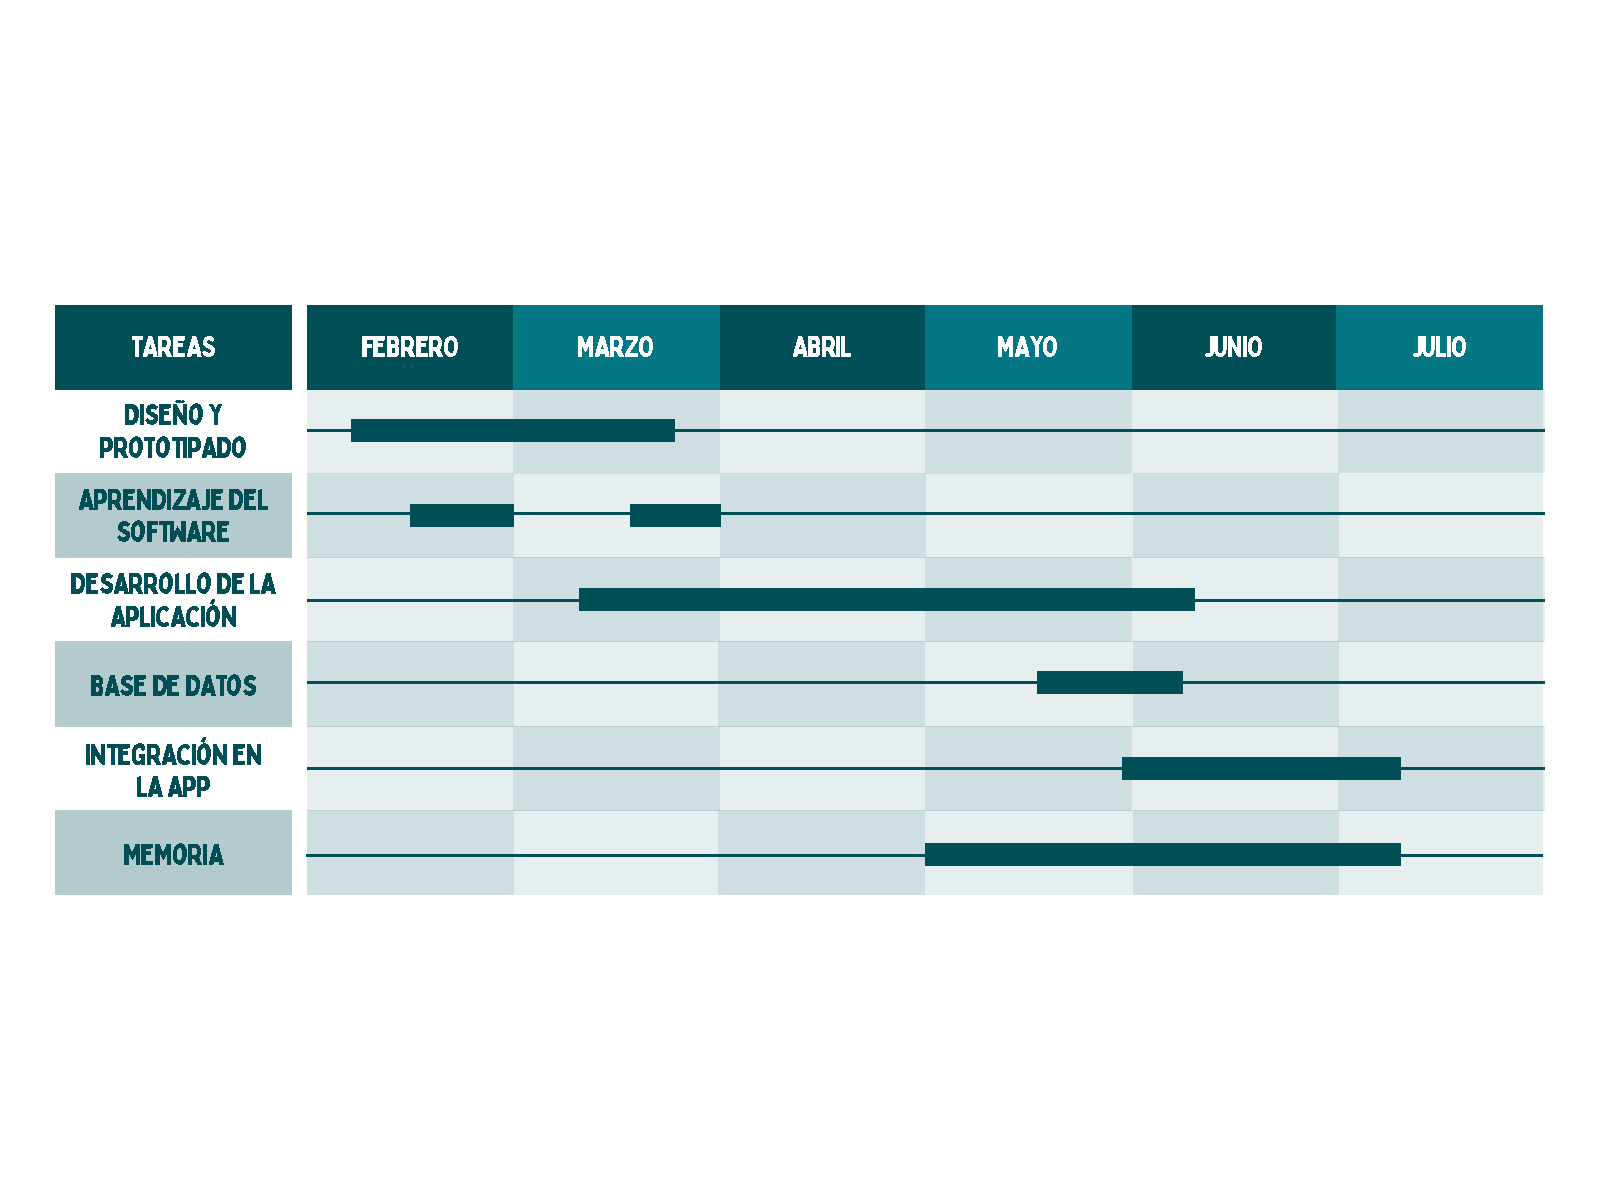
\includegraphics[width=1.0\textwidth]{images/EjemploGantt.pdf}
    \caption{Diagrama de Gantt\label{fig:gantt}}
\end{figure}

En ella se puede observar que hay seis tareas en el proyecto y que el mismo se desarrolla desde febrero a julio. A modo de ejemplo, el \textit{Diseño y prototipado} se llevará a cabo desde la segunda semana de febrero hasta la tercera semana de marzo. Además, en este diagrama hay tareas que se pueden hacer en paralelo (como el diseño y prototipado y el aprendizaje del software, entre otras). % Modificar el diagrama para poner alguna tarea secuencial para indicarlas.

El diagrama de Gantt debe incluir todas las tareas que has realizado (o vas a realizar, pues es se hace antes de comenzar a realizar las tareas) vinculadas con los objetivos del TFG. Ten en cuenta que en los objetivos de tu TFG no debe haber solo objetivos de desarrollo, sino también en muchos casos de aprendizaje, porque te plantees aprender nuevas tecnologías o conocer más del dominio de aplicación del problema que vas a abordar. También tendrás objetivos relacionados con la organización de tu trabajo como reuniones, revisiones y redacción de la memoria. Teniendo en cuenta esto, debes planificar todas las tareas necesarias para cubrir los objetivos planteados, y por ello, en el cronograma debe haber tareas de aprendizaje, de desarrollo, y de organización. En cuanto al desarrollo, si vas a seguir una metodología específica, esta tiene que verse reflejada en el cronograma. Por ejemplo, si sigues una metodología ágil con iteraciones cada dos semanas, en tu cronograma debería aparecer una tarea con duración de dos semanas por cada iteración. Si tu ciclo de vida no es iterativo sino clásico, deberían aparecer paquetes de trabajo para análisis, diseño, implementación, pruebas, etc, con tareas específicas dentro de cada uno de ellos.

Cuanto mayor sea el nivel de detalle del cronograma, mejor, ya que darás más información de las tareas y tiempo dedicados. Te aconsejamos que la unidad temporal usada en el cronograma sea semanal, aunque también puedes usar meses. 

Existen varias aplicaciones informáticas de escritorio o en línea para hacer diagramas de Gantt y gestionar cambios sobre estos. Muchas de estas herramientas permiten fijar una línea base (como una fotografía del diagrama en un momento) para comparar con cambios posteriores, de tal forma que también se pueden hacer simulaciones. Otra funcionalidad que ofrecen estas herramientas es poder asignar recursos humanos y materiales a las tareas, con costes asociados, lo cual es muy útil para hacer un presupuesto del proyecto. Algunas de estas aplicaciones te permiten trabajar en equipo haciendo un uso compartido entre varios usuarios. En tu caso podrías compartir el diagrama de planificación con la persona que te tutoriza.

A día de hoy, te podemos sugerir algunas herramientas gratuitas y sencillas para hacer y gestionar diagramas de Gantt, como son \href{https://www.ganttproject.biz/}{GanttProject}, \href{https://www.projectlibre.com/}{Project Libre}, 
 \href{https://www.monday.com}{Monday.com}, \href{https://app.clickup.com/}{Clickup}. 

También puedes hacer tu diagrama de Gantt usando \href{https://www.canva.com/}{Canva}, eligiendo una de las plantillas de este tipo que se proveen, o con una hoja de cálculo, pero en estos casos no tienes tantas facilidades para editar los cambios temporales, ni funcionalidades como las apuntadas arriba.

Algunas recomendaciones sobre esta sección son que describas brevemente los tipos de tareas de tu diagrama y cuál es tu metodología de desarrollo para que se pueda comprender mejor. En cuanto a su visualización dentro de la memoria, debes asegurarte de que el diagrama se vea bien, para lo cual te sugerimos que lo pongas en apaisado a página completa, o que lo subdividas en varios diagramas (por ejemplo, uno por cada paquete de trabajo). El diagrama deberá formar parte de la presentación final, así que es mejor que uses colores o tramas para diferenciar mejor los tipos de tareas y para que sea más atractivo visualmente. Y no está de más que lo describas textualmente, explicando y justificando la distribución, las restricciones y las dependencias temporales entre las tareas.

Llegado este punto hay que distinguir qué es una planificación de una representación temporal real del desarrollo del proyecto. La primera se hace a priori, antes de empezar a trabajar. Es una planificación de lo que se va a realizar en el futuro. Sin embargo, la segunda es una fotografía real de lo que se ha hecho, con las desviaciones temporales y cambios que ha habido durante el desarrollo del proyecto. En definitiva es un cronograma que refleja la realidad de lo que ha acontecido. Para realizarlo, te aconsejamos que vayas apuntando el número de unidades temporales que has dedicado realmente a cada tarea en un diario y que confecciones un diagrama de Gantt con toda la información. Este segundo diagrama podría ir en una subsección en el capítulo correspondiente de conclusiones, donde además indicarás las desviaciones, si es que han ocurrido, y el porqué de ellas. Este ejercicio te servirá para que compruebes qué capacidad de planificación real tienes (cuánto de optimista o pesimista, o justo, has sido a la hora de planificar tareas). Y también para detectar tareas problemáticas o cuellos de botella. El análisis de las mismas y de las posibles desviaciones te hará aprender y poder planificar con más precisión en futuros proyectos. 

%OJOJOJOJOJOJOJJOJOJOJOJ ESTO NO LO VEO -> DEBE HACERSE A PRIORI
%Te será muy fácil hacer el cronograma si has sido metódico/a, apuntando cada día de trabajo en el TFG el número de horas dedicadas al TFG y a qué tarea específica las has dedicado. Solo recuerda que todo el tiempo de tu vida que dediques al proyecto debe estar reflejado en el cronograma final. 


\section{Plan de gestión de riesgos y contingencias}

En algunos TFG, por su temática o tecnologías usadas, o porque la persona que te tutoriza lo vea conveniente, se puede presentar un plan de gestión de riesgos. El plan es una lista de posibles riesgos que pueden surgir durante el desarrollo del TFG, cada uno de ellos con acciones para evitarlos y/o mitigarlos. 

La lista de riesgos suele priorizarse según su impacto en el proyecto. Para ello, hay que hacer un estudio previo en el que valoremos si la ocurrencia del riesgo afecta al alcance del TFG (cambios en requisitos), al tiempo (retrasos, cambio de orden y tiempo asignado a tareas), al coste (incremento de gastos), a los recursos (cambios en tecnología usada), etc. Una vez valorado esto, asignaremos más prioridad a aquellos que tengan mayor impacto. 

Teniendo en cuenta el impacto de cada riesgo, lo siguiente es planificar una acción de prevención para evitar que ocurra, si es posible. Se deben planificar acciones de mitigación si no podemos evitar que el riesgo ocurra o si el plan de prevención fallara.

Por ejemplo, un riesgo podría ser que la tecnología a usar para el desarrollo del TFG sea muy nueva, lo que conlleva que no haya apenas manuales de uso y poca gente la conozca, así que no podrás tener mucha ayuda en foros, y  si tienes algún problema con ella puede que no puedas seguir adelante y te quedes bloqueado. El impacto de ese riesgo podría afectar al alcance del proyecto, pero también al tiempo y por supuesto a los recursos. Como plan de prevención, podrías apuntarte a un curso de formación existente (aunque incremente los costes del proyecto), y como plan de mitigación, la acción propuesta podría ser dejar el uso de esa tecnología solo para una parte del desarrollo menos importante, no para todo, de tal forma que no se vea afectado el proyecto completo.

Tienes una lista de diversos tipos de riesgos y más información sobre el plan de gestión de riesgos en el capítulo de Estimación de riesgos, de \cite{guerin2018gestion}, disponible en línea en la biblioteca de la UGR.

Una vez planteado el plan de mitigación, durante el proyecto debe revisarse para decidir si se realiza alguna de las acciones previstas y en esta sección de la memoria, explicar con detalle qué acciones se han realizado y sus resultados, incluyendo comentarios sobre los costes asociados.

Si vas a incluir un plan de gestión de riesgos, consensúa con la persona que te tutoriza en qué capítulo incluirlo, ya que una opción es que sea una sección del capítulo de la propuesta, para que esté más cercano a la explicación de  cómo se han gestionado los riesgos durante el desarrollo.

\section{Presupuesto}

Con esta sección se indica al lector de la memoria cuál sería el coste de desarrollo del proyecto realizado dentro del TFG en el caso de que este proyecto se ejecutara en la vida real. Esta sección ayuda al lector valorar el tiempo dedicado por tu parte al proyecto, tus decisiones respecto a la tecnología elegida, y el coste de todo ello. Como ingeniero, debes demostrar que sabes hacer un proyecto coherente  y sensato, buscando las mejores alternativas. 

El presupuesto debe tener dos tipos de conceptos principales: costes de personal y costes de ejecución.

El personal que realiza el proyecto eres tú, por lo que el coste se calcula multiplicando el número de horas que tú has dedicado al TFG por el coste por hora estimado. Si para el desarrollo de tu proyecto has tenido que aprender tecnologías y revisar un estado del arte, ese tiempo también debe cuantificarse. Es decir, en el coste final debes contar también las horas que no son exclusivamente de desarrollo. Y también, como sucede en la mayoría de los casos, deberás contabilizar por separado las horas de análisis y diseño de las horas de implementación, que normalmente tienen un costo diferente. ¿Cómo puedes estimar el coste por hora según el tipo de rol profesional? Te recomendamos que consultes en portales de empleo o sitios especializados, mirando los anuncios, o usando, si las proporcionan, herramientas de cálculo de salarios brutos anuales según ciudad, o publicaciones sobre los salarios medios según la categoría profesional, como las siguientes: \href{https://www.tecnoempleo.com/ofertas-trabajo/}{TecnoEmpleo} o \href{https://www.tecnoempleo.com/ofertas-trabajo/}{InfoJobs}, o en el cluster de empresas tecnologícas de Granada, \href{https://www.ontechinnovation.com/bolsa-de-trabajo/}{On Granada Tech City}. Cuando hagas la consulta, ten en cuenta que no todos los informáticos cobran lo mismo, ni en todas las ciudades. Tu categoría será posiblemente \textit{junior}, sin experiencia previa en trabajo. 

Las reuniones que mantengas con tu tutor también deben computarse como tiempo dedicado y debes computar también en el coste total las horas dedicadas por tutor (al correspondiente precio/hora, quizá equiparable al de un consultor). Si tu proyecto implica reuniones con el cliente, estas deben aparecer igualmente.

% OJOJOJOJOJOJOJOJOJJO EL PRESUPUESTO SE HACE A PRIORI, POR TANTO NO SE TIENE EN CUENTA EL NÚMERO DE HORAS REALES DEDICADAS AL PROYECTO. 
Para el cálculo total de horas ya te hemos recomendado que lleves un diario donde las anotes. Tiene que haber coherencia entre tu planificación temporal y número de horas dedicado al proyecto, y el número de horas que pones en esta subsección.

Respecto a los costes de ejecución, aquí debe ir una línea por cada uno de los gastos hardware, software, viajes y dietas que preveas tener durante el desarrollo del TFG. 

En cuanto al hardware, puedes incluir el coste de dispositivos usados como tu ordenador, tablet, teléfono, etc. pero no el coste íntegro. Piensa que esos dispositivos los has usado para otros proyectos, incluidos los personales, por lo que debes prorratear teniendo en cuenta su tiempo de vida útil, el coste actual del dispositivo en el estado en el que está y el tiempo de vida de uso exclusivo para el proyecto. Por ejemplo, si un portátil te costó 600 euros en su día, y hoy valdría 400 euros, y le quedan dos años de vida útil, pero tú lo has usado solo 6 meses para este proyecto, podrías anotar en el coste de ejecución asociado a equipamiento unos 100 euros como mucho.  

Por otro lado, si para tu TFG has necesitado cualquier material hardware aparte, que hayas tenido que adquirir o te haya facilitado la persona que te tutoriza, también debes incluirlo (con su prorrateo si es el caso). Si has tenido que contratar un servidor, añade también los costes según los meses que lo vayas a usar, y prevé el coste un uso de un año más para dar soporte al proyecto y su mantenimiento. Lo mismo si necesitas adquirir o contratar software.

Si necesitas viajar para realizar tu TFG, también puedes incluir como gastos de ejecución los costes de dietas y desplazamiento. Esto suele incluirse en TFGs de investigación o más aplicados, que requieren reuniones con colaboradores como entidades o empresas que han solicitado que se realice un TFG con ellas y que actúan como nuestros clientes, dando requisitos, evaluando diseños y haciendo pruebas. 

Por último, puedes añadir costes indirectos. Son aquellos que se comparten entre varios proyectos, como la electricidad o cuota de Internet. Normalmente se calcula un 10\% del total del presupuesto para costes indirectos.

El presupuesto lo puedes hacer en una tabla pero te aconsejamos que lo hagas mejor con una herramienta como una hoja de cálculo, o una de gestión de proyectos que haga cálculo con los costes de recursos y planificación temporal, como las mencionadas en la subsección anterior.

Como consejo, no añadas únicamente la tabla del presupuesto a la memoria, añade un texto breve explicativo, incluyendo alguna justificación sobre los gastos como en qué te has basado para el cálculo de coste por hora, o porqué se ha adquirido y usado cierta tecnología que mencionas en el presupuesto. Si durante el proyecto has cambiado de tecnología y ésto ha influido en los costes, menciónalo también.

Por último, y como te hemos indicado en la planificación, anota los costes reales de tu proyecto, inclúyelos, por ejemplo, como una sección de conclusiones y comenta y justifica las desviaciones. La diferencia entre el presupuesto y el costo real no debería ser muy grande. Si es así, has sido muy optimista a la hora de dar un presupuesto y esto también tendrás que entrenarlo.

\subsection{Ejemplo de presupuesto}

\subsection{Coste de desarrollo}

\subsubsection{Coste de personal}

\subsubsection{Coste de material}

\subsection{Coste de despliegue y mantenimiento}
\chapter{Las conclusiones y los trabajos futuros}
\label{cap:Conclusiones}

% [Autores: María José Rodríguez Fórtiz]
El capítulo de Conclusiones y Trabajos Futuros es muy importante pues recoge qué se ha realizado en el TFG, los principales resultados, y qué puede hacerse a partir de este momento. Muchas personas leen la introducción y luego las conclusiones antes de leerse el resto de la memoria, para así conocer bien la motivación, objetivos y los resultados del trabajo.

Eso significa que debes tener especial cuidado al redactar este capítulo para que quede muy claro y sea muy completo.

Habitualmente incluye dos secciones, la de conclusiones y la de trabajos futuros.
 
 \section{Conclusiones}

Debes empezar las conclusiones con una frase inicial a modo de resumen sobre los resultados de tu trabajo, con una valoración positiva sobre ellos. 

A continuación debes hacer un repaso uno a uno de los objetivos específicos, indicando en ese repaso: (1) el porcentaje de realización, (2) un resumen de lo que se ha hecho para cumplir ese objetivo (dos o tres líneas explicando las tareas realizadas asociadas a ese objetivo, y los resultados obtenidos deben bastar), y (3) una indicación de dónde pueden verse las evidencias de ese objetivo en la memoria, en qué capítulo o sección.

También puedes mencionar en esta parte, cómo tu formación previa en materias concretas del grado te ha sido de ayuda para el TFG. 

 En cuanto a la redacción de este repaso de objetivos, te ponemos un ejemplo. Suponiendo que estás abordando un objetivo específico que has redactado como "Revisar aplicaciones similares para comparar con la propuesta", puedes indicar que ese objetivo se ha cumplido completamente, explicando por ejemplo que has revisado 6 aplicaciones similares y que has realizado una tabla comparando 8 características básicas de cada una, la cual puede consultarse en el capítulo o sección X de la memoria. También puedes añadir que al elaborar esta tabla se demuestran tus capacidades de análisis y síntesis de información. Si este objetivo no se hubiera cumplido completamente, porque, por ejemplo solo hayas revisado 2 aplicaciones y tenías previsto revisar más, pues dices lo que sí has hecho pero solo un 30\%, y argumentas porqué es insuficiente, por ejemplo porque solo hay 2 de libre acceso que has podido consultar con profundidad, o porque has priorizado terminar la tarea X, que habéis considerado que era más importante para el TFG. 

 De cara a la redacción de esta sección puedes tener en cuenta el registro de marcas propuesto en \cite{meza2019comunicacion} \textcolor{orange}{, que sugiere verbos que puedes utilizar (en este caso para explicar en las conclusiones cuál ha sido el alcance de cada objetivo), como son: "se ha abordado", "hemos hecho un recorrido por", "podemos afirmar que", "esto evidencia que", "confirmamos que", "confirma nuestras hipótesis/ideas", "hemos propuesto/obtenido/identificado/revisado/observado/descubierto/utilizado/demostrado/explicado/desarrollado ...",  "no hemos podido demostrar/confirmar/revisar/identificar ... porque ...", etc. Como marcadores discursivos, podemos usar conectores como los siguientes: "por tanto", "sin embargo", "en consecuencia", "por el contrario", "a pesar de", "gracias a", "entendemos que", o "de acuerdo/según todo lo anterior".}
 
Es importante que en las conclusiones añadas un párrafo final como valoración personal, escrito esta vez en primera persona. En esa valoración debes mencionar cómo te has sentido al realizar el TFG y en base a sus resultados. Puedes indicar que te sientes orgulloso/a, contento/a, satisfecho/a, encantado/a, etc. por lo que has aprendido, por cómo te has organizado en el tiempo, por cómo has redactado la memoria, por la calidad del código desarrollado, por cómo te has comunicado con tu tutor, etc. Si tienes alguna valoración negativa, debes mencionarla también, pero te recomendamos que la redactes de forma positiva, aportando que has aprendido de ello. Por ejemplo, "No estoy satisfecho/a con cómo he organizado el trabajo temporalmente porque he dejado muchas tareas para el último mes y eso me ha saturado, con lo cual he aprendido que en un futuro debo hacer una mejor planificación temporal desde el principio.". En tu valoración personal, y si no lo has hecho al revisar los objetivos, también puedes mencionar cómo has aplicado y mejorado tus habilidades blandas o soft skills, como son organización de trabajo, pensamiento crítico, creatividad, adaptación, resolución de problemas y comunicación. 

 \section{Trabajo futuro}

 En esta sección se enumeran:
 \begin{itemize}
     \item Tareas que que estaban previstas y no se han hecho o han quedado incompletas, de las mencionadas en las conclusiones
     \item Requisitos de desarrollo que tenías previsto abordar pero que al final no has tratado
     \item Nuevos requisitos que hayan surgido durante el desarrollo del TFG, que no se habían previsto y por tanto no se han planificado ni abordado
     \item Nuevos objetivos e ideas para dar continuidad al TFG en futuros TFGs, desarrollos o investigaciones.
 \end{itemize} 

 Para cada una de estas tareas, requisitos u objetivos conviene añadir un pequeño párrafo que explique porqué se propone y cómo se abordaría, de forma muy resumida. Por ejemplo: "En un futuro se puede desarrollar una versión en iOS del prototipo realizado en el TFG. Esto ayudaría a que más personas pudieran utilizar la aplicación. Para ello, se podría utilizar un framework de desarrollo como Flutter o Ionic, que permiten esta portabilidad y el desarrollo híbrido de aplicaciones móviles. Habría que valorar si el código actual o parte de éste puede reutilizarse". Otro ejemplo de párrafo: "Sería necesario completar la gestión de usuarios en la aplicación desarrollada, ya que por el momento solo pueden hacerse altas y modificaciones. Bastaría para ello diseñar e incluir funciones e interfaces para el borrado de usuarios de la misma forma que se ha hecho para las otras operaciones. Esto no supondría ningún cambio en la base de datos". 

 

 
\chapter{La bibliografía\label{cap:bibliografia}} % [Autores: Rocío Romero Zaliz] 

% Definición y propósito
% Importancia de la bibliografía en un TFG/TFM
La bibliografía es un componente esencial de un trabajo fin de carrera, tanto de grado como de posgrado, ya que no solo justifica y respalda tus argumentos, sino que también enriquece tu trabajo al proporcionar acceso a fuentes adicionales de información. Por tanto, es importante que dediques el tiempo necesario para elaborar una bibliografía completa y correctamente formateada.

\section{¿Por qué citar?}

Citar es una práctica fundamental en cualquier trabajo académico. Se trata de mencionar las fuentes de información que se han utilizado en tu trabajo ya que, además de constituir un reconocimiento hacia ellos/ellas, las citas académicas permiten distinguir claramente cuáles son tus aportaciones y en qué se sustentan. Citar el trabajo de otros/as autores/as te permite:

\begin{itemize}
    \item Contextualizar el tema de estudio, situándolo dentro de un marco teórico que ayude al lector a comprender mejor tu trabajo y su relevancia en ese contexto.
    \item Demostrar dominio del tema que abordas gracias a todo el trabajo de documentación realizado, aumentando la credibilidad en tu trabajo.
    \item Permitir la verificación de la información utilizada, algo indispensable para  garantizar la transparencia y la confiabilidad de tu trabajo.
    \item Respaldar tus argumentos mediante citas de fuentes confiables y relevantes, aumentando la credibilidad en un trabajo.
    \item Ampliar la información con recursos adicionales que ofrezcan al lector la posibilidad de profundizar en el tema de estudio, enriqueciendo tu trabajo y volviéndolo más completo e informativo.
\end{itemize}

\section{¿Qué citar?}

Es importante citar siempre que se utilice información de otra fuente. Esta información puede ser:

\begin{itemize}
    \item Una {\em cita textual} cuando se copia una frase o párrafo palabra por palabra.
    \item Una {\em paráfrasis} cuando se presenta una idea de otra fuente con tus propias palabras.
    \item Datos o estadísticas, tanto en forma de números individuales como de tablas completas o parciales.
    \item Material gráfico que no hayas generado tú, incluso en caso de rehacer una imagen de otro/a autor/a por querer cambiarle los colores o el tipo de letra, debes indicar cuál es la fuente original en qué te has basado. 
    \item Software o recurso en línea.
    \item Código fuente reutilizado de otros/as autores/as.
\end{itemize}

\section{¿Cómo citar?}

En caso de realizar una cita textual debes colocar ese texto entre comillas. En caso de citar una frase o proverbio, del cual no se tenga una referencia bibliográfica, se puede indicar en el texto, antes o después, quién es su autor/a. Esto también es válido para comunicaciones personales:

\begin{quote}
\begin{it}
    No olvides la famosa frase de Confucio ``Aprende a vivir y sabrás morir bien''.
\end{it}
\end{quote}

En caso de hacer referencia a una cita textual de la cual si se tiene conocimiento del origen de ese texto, es necesario citarlo colocando una referencia a la bibliografía tras el entrecomillado. Las referencias a la bibliografía pueden tener distintos formatos, en el siguiente ejemplo puedes verlo indicado por un número entre corchetes que se enlaza a la bibliografía donde se incluyen todas las referencias bibliográficas:

\begin{quote}
\begin{it}
     Es importante mencionar un estudio que ``...revela que cualitativamente las guías docentes incluyen competencias que posteriormente no están consideradas...'' \cite{fernandez2023evaluacion}.
\end{it}
\end{quote}

Cuando realices alguna paráfrasis simplemente escribe tu texto y al final de la frase o párrafo colocas la referencia a la bibliografía:

\begin{quote}
\begin{it}
     Un estudio indica que las guías docentes consideran competencias luego se ignoran \cite{fernandez2023evaluacion}.
\end{it}
\end{quote}

Si escribes varios párrafos basados en el trabajo de otro/a autor/a coloca la referencia en el último párrafo:

\begin{quote}
\begin{it}
    El segundo hallazgo se centra en el análisis de la correspondencia entre las competencias descritas en las guías docentes y las rúbricas de evaluación. Este estudio pone de manifiesto que, cualitativamente, las guías docentes incluirán competencias que posteriormente no se reflejan en los ítems específicos de las rúbricas.
    
    Sorprendentemente, este fenómeno no es una excepción, sino más bien una tendencia generalizada a nivel nacional. La discrepancia entre las competencias propuestas y las evaluadas plantea interrogantes sobre la coherencia y la eficacia de los procesos de evaluación en los Trabajos Fin de Grado (TFG) en el ámbito de la Ingeniería Informática en España \cite{fernandez2023evaluacion}.
\end{it}
\end{quote}

En el caso de tener que hacer referencia a una figura o tabla puedes colocar la referencia bibliográfica en la leyenda de la misma. En caso de que tu figura o tabla no esté copiada textualmente y haya servido de inspiración o bien has recogido un subconjunto de la información puedes indicarlo en la leyenda:

\begin{table}[!ht]
    \begin{varwidth}[b]{0.45\linewidth}
        \centering
            \begin{tabular}{c c}
            \toprule
            \textbf{Pregunta} & \textbf{\%} \\
            \midrule
            ¿Las rúbricas consideran & \\
            la evaluación del tutor? & 59\% \\
            ¿Las rúbricas establecen & \\
            la ponderación de los ítems? &  66\% \\
            ¿Las rúbricas detalla los & \\
            rangos de calificaciones? & 34\%  \\
            \bottomrule
        \end{tabular}
        \caption{Resumen de hallazgos en las rúbricas tomados de \cite{fernandez2023evaluacion}.}
        \label{tab:rubricas}
       \end{varwidth}\hfill
    \begin{minipage}[b]{0.5\linewidth}
        \centering
        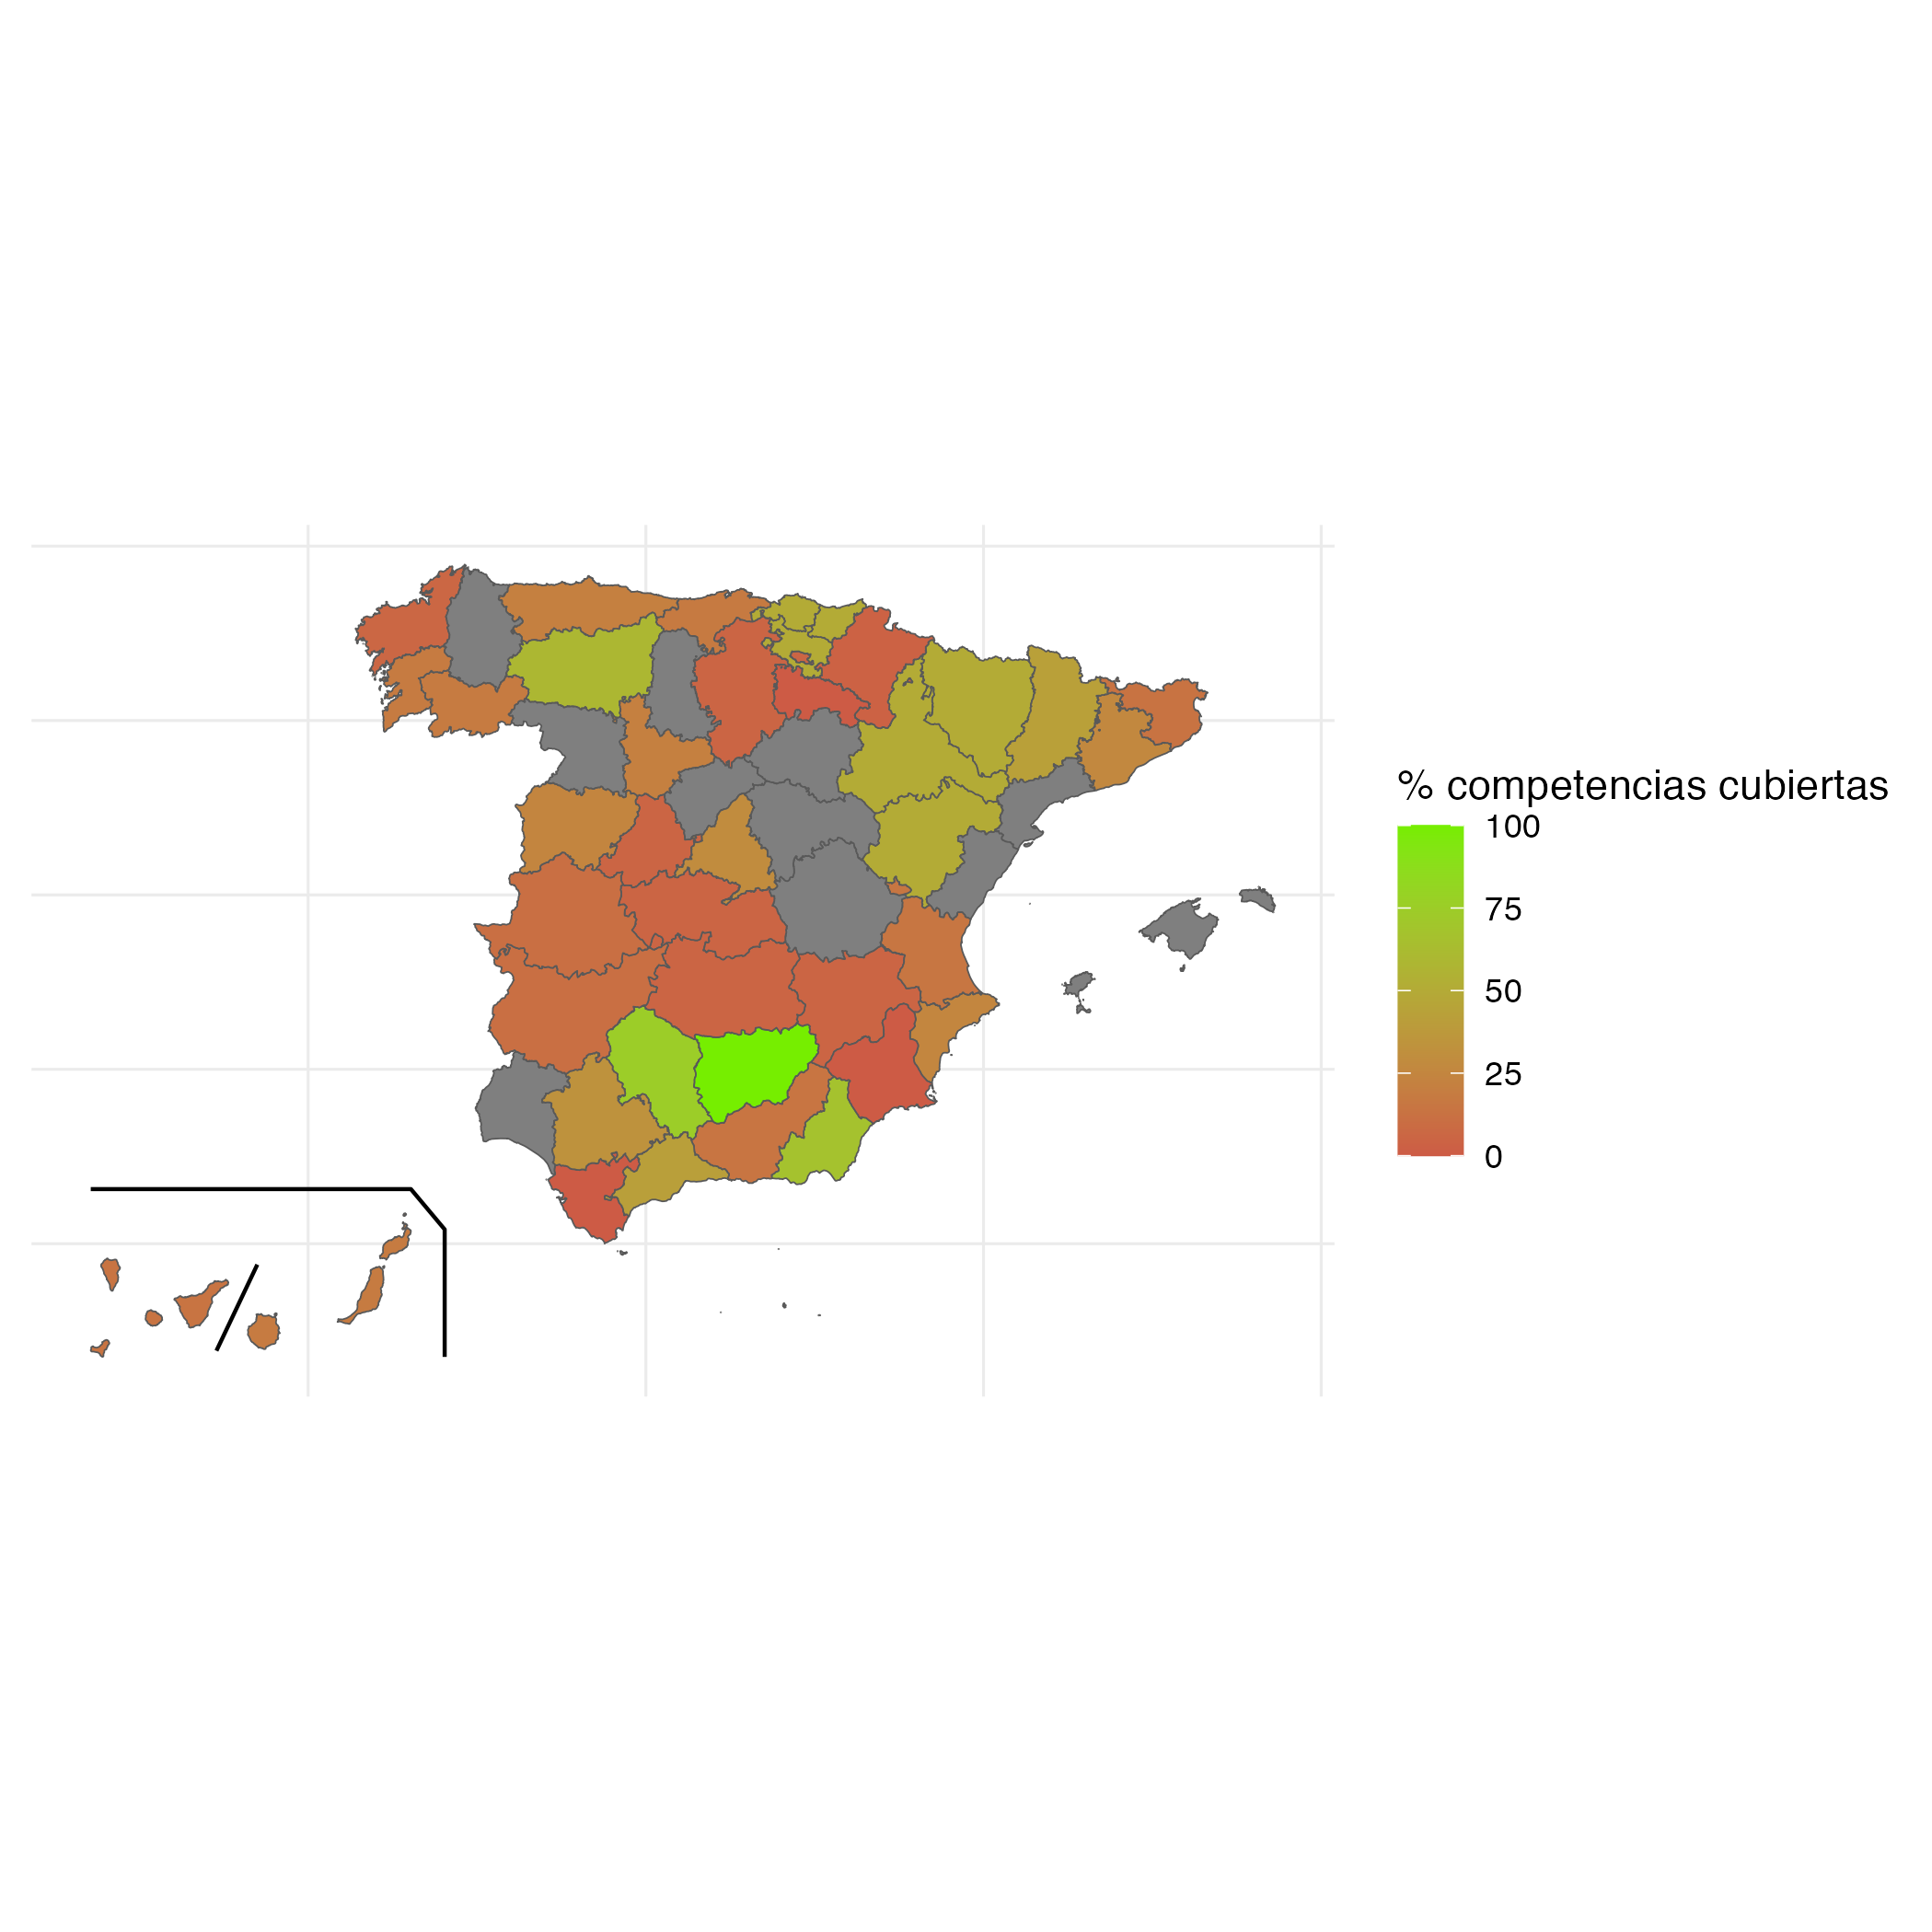
\includegraphics[scale=0.5, trim={0 5cm 5cm 5cm}, clip]{images/Mapa_prov.png}
        \captionof{figure}{Mapa de rúbricas basado en \cite{fernandez2023evaluacion}.}
        \label{fig:image}
    \end{minipage}
\end{table}

En caso de querer referenciar una página web, puedes hacerlo directamente en la bilbiografía con el resto de elementos. En caso de tener pocas referencias a páginas web puedes optar por incluirlas directamente como un pie de página o entre paréntesis. Ten en cuenta que dependiendo de la página web a la que hagas referencia puede ser necesario indicar el momento en que se ha accedido a esta información, especialmente si ésta se actualiza frecuentemente:

\begin{figure*}[!ht]
    \begin{minipage}{.45\textwidth}
        \begin{it}
        Para mas información puedes consultar la página web del Instituto Nacional de Estadística (https://ine.es/index.htm).
        \end{it}
    \end{minipage}
    \hfill
    \begin{minipage}{.45\textwidth}
        \begin{it}
        Para mas información puedes consultar la página web del Instituto Nacional de Estadística$^1$\\
        --\\
        $^1$ https://ine.es/index.htm. Accedido el 14 de febrero de 2024.
        \end{it}
    \end{minipage}
\end{figure*}

En caso de tener muchas referencias se recomienda tener un apartado de bibliografía exclusivo para los enlaces web y simplemente usar una referencia en el texto:

\begin{quote}
\begin{it}
    Para mas información puedes consultar la página web del Instituto Nacional de Estadística \cite{INE}.
\end{it}
\end{quote}

\begin{table}[!hbt]
    \centering
    \begin{minipage}{0.48\linewidth}
        \centering    
        \begin{tabular}{r|l}
            \toprule
            Referencia a & Información \\
            \midrule
            Libro & Autores/as \\
            & Título \\
            & Editorial \\
            & Año de publicación \\
            & {\it ISBN} \\
            & {\it Edición} \\
            \midrule
            Capítulo & Autores/as\\
            de Libro & Título del libro\\
            & Título del capítulo\\
            & Editorial\\
            & Año de publicación\\
            & {\it ISBN} \\
            & {\it Edición} \\
            \midrule
            Artículo & Autores/as\\
            científico & Título\\
            en revista & Nombre de la revista\\
            & Volumen \\
            & Año de publicación\\
            & {\it Número} \\  
            & {\it Páginas} \\
            & {\it DOI} \\
            \bottomrule
        \end{tabular}
    \end{minipage}%
    \hfill
    \begin{minipage}{0.48\linewidth}
        \centering
        \begin{tabular}{r|l}
            \toprule
            Referencia a & Información \\
            \midrule
            Artículo & Autores/as\\
            científico & Título\\
            en congreso & Nombre del congreso\\
            & Año de publicación\\
            & {\it Lugar} \\
            & {\it Fechas} \\
            & {\it Páginas} \\
            \midrule
            TFG & Autor/a\\
            TFM & Título \\
            Tesis doctoral & Universidad \\
            & Tipo \\
            & Año de publicación \\
            & {\it Tutor} \\
            \midrule
            Software & Nombre \\
            & Versión \\
            & {\it Enlace web} \\
            \midrule
            Página web & Título \\
            & Autores \\
            & Enlace web \\
            & Fecha de último acceso \\
            \bottomrule
        \end{tabular}
    \end{minipage}
    \caption{Información mínima y opcional (en itálica) para cada tipo de referencia a citar.}
    \label{tab:citar}
\end{table}

Si bien tienes estas tres opciones para referenciar contenido en línea, no debes usar más de una en tu memoria, elige la más conveniente y usa ese estilo para todas las referencias.

Si necesitas citar un software específico recuerda indicar la versión utilizada. Puedes adicionalmente agregar si quieres una referencia a la página web de la empresa o proyecto relacionado:

\begin{quote}
\begin{it}
    Para este trabajo se ha utilizado el lenguaje de programación Julia v1.10.0 (https://julialang.org/) \cite{bezanson2017julia}.
\end{it}
\end{quote}

En caso de reutilizar código fuente de otras personas indícalo tanto en el texto de la memoria, enlazando con la página web de donde has descargado esa información, como en tu propio código fuente mediante un comentario en la cabecera de la función o paquete donde se encuentre.

\begin{quote}
\begin{it}
    En este trabajo se ha reutilizado parte del código fuente del proyecto TSFEDL (\url{https://github.com/ari-dasci/S-TSFE-DL}), más detalles en el repositorio GitHub de este trabajo fin de grado (\url{https://github.com/mitfg/}).
\end{it}
\end{quote}

Para el resto de referencias, sean libros, artículos científicos u otros trabajos fin de carrera, la referencia bibliográfica deberá tener unos u otros componentes básicos dependiendo del tipo de referencia. En la Tabla \ref{tab:citar} puedes ver la información mínima y opcional (en itálica) para cada tipo de cita posible.
    
\begin{naranja}
Existen muchos formatos de citas, algunas usan números entre corchetes para referenciarlos, otros utilizan el nombre del primer autor y el año entre paréntesis, etc. Luego, dependiendo del formato se colocarán las referencias en la bibliografía en un cierto orden: orden alfabético, en el orden en que fueron citadas, etc. Estos formatos siguen distintas normativas o estilos. Las más conocidas son:

\begin{itemize}
    \item APA (American Psychological Association): En este formato, las referencias en el texto utilizan un sistema de citación por autor y fecha. Todas las citas que aparecen en el texto deberán luego ordenarse alfabéticamente. Este estilo se diseñó originalmente para trabajos en psicología, pero se han extendido a otros campos como la educación y las ciencias sociales debido a su claridad y facilidad de uso. Un ejemplo de este formato es:
    \begin{quote}
        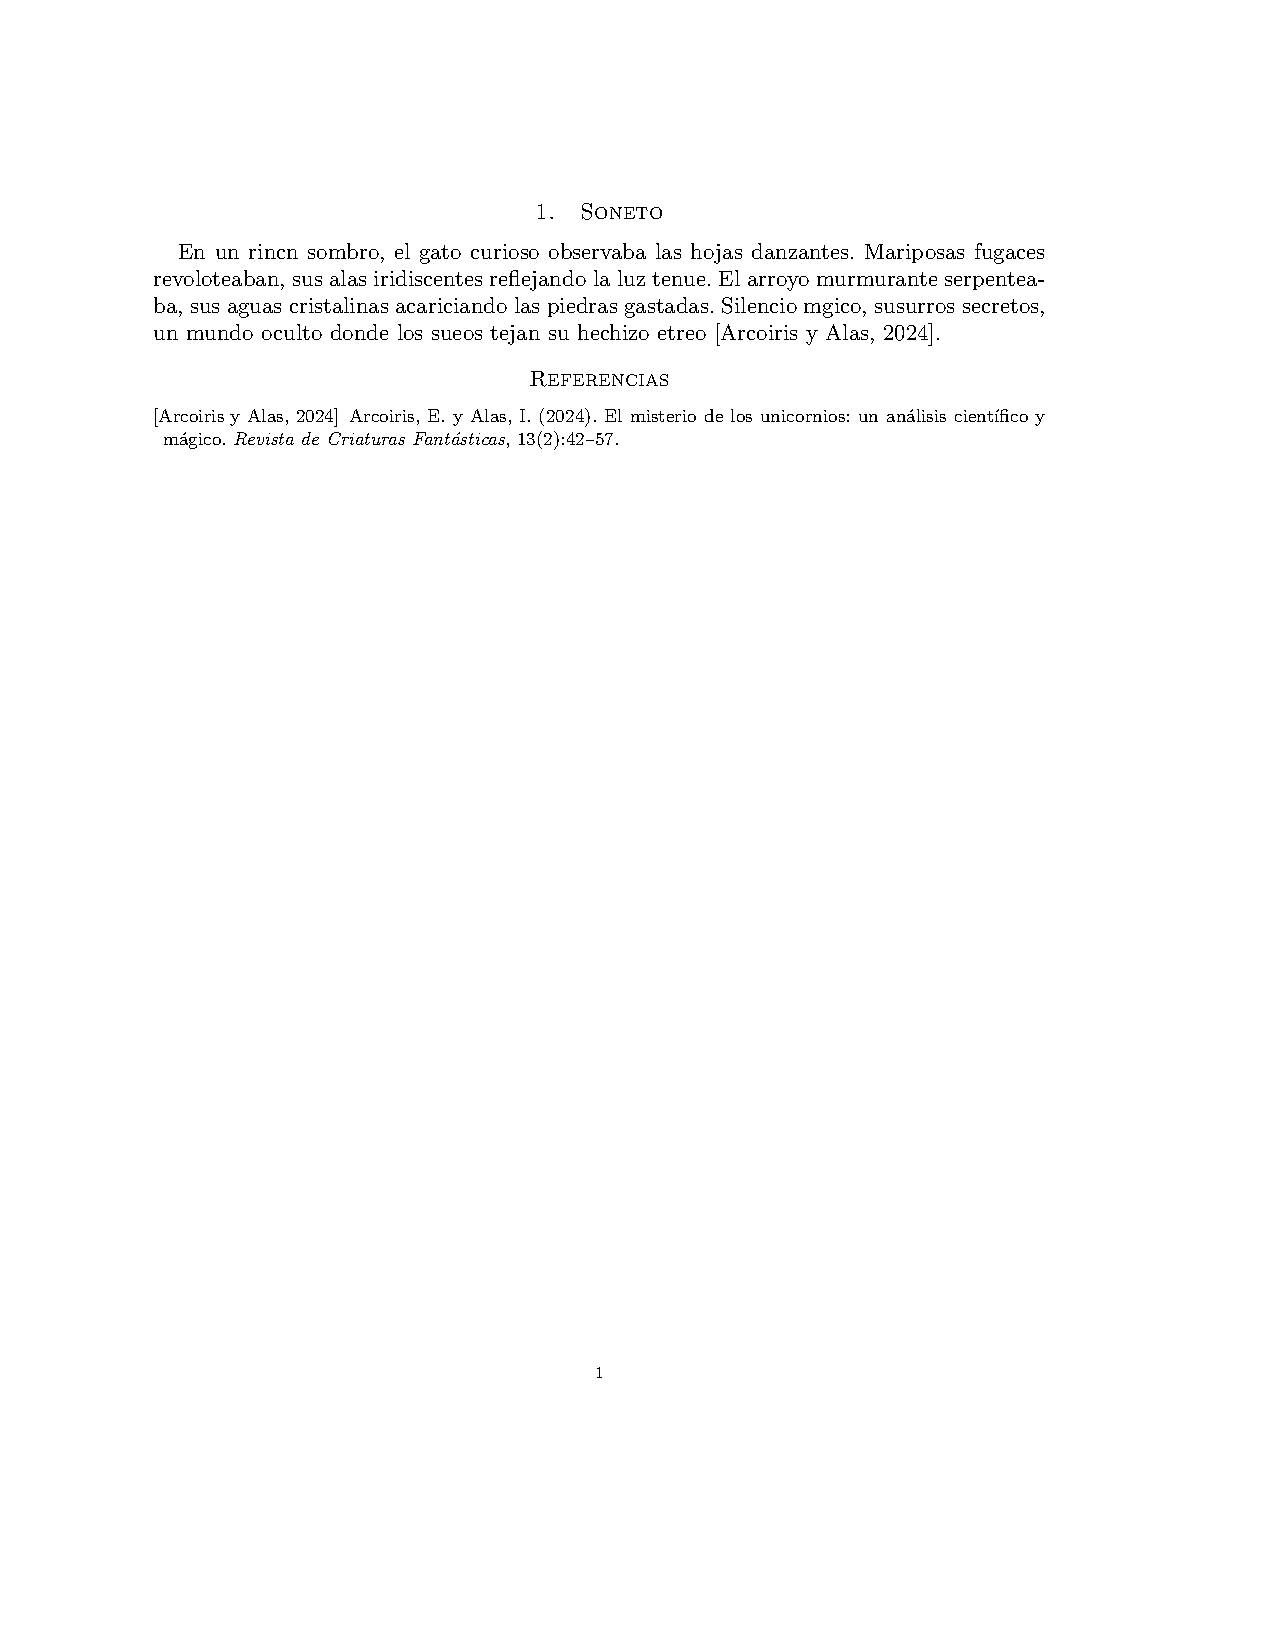
\includegraphics[scale=0.6, trim={2cm 20cm 3cm 3cm}, clip]{images/apa.pdf}
    \end{quote}
    \item MLA (Modern Language Association): En este formato, las citas dentro del texto no incluyen la fecha como en otros estilos, solo llevan el nombre del primer autor entre paréntesis. Es ampliamente utilizado en el ámbito de las humanidades, lengua y literatura. Un ejemplo de este formato es:
    \begin{quote}
        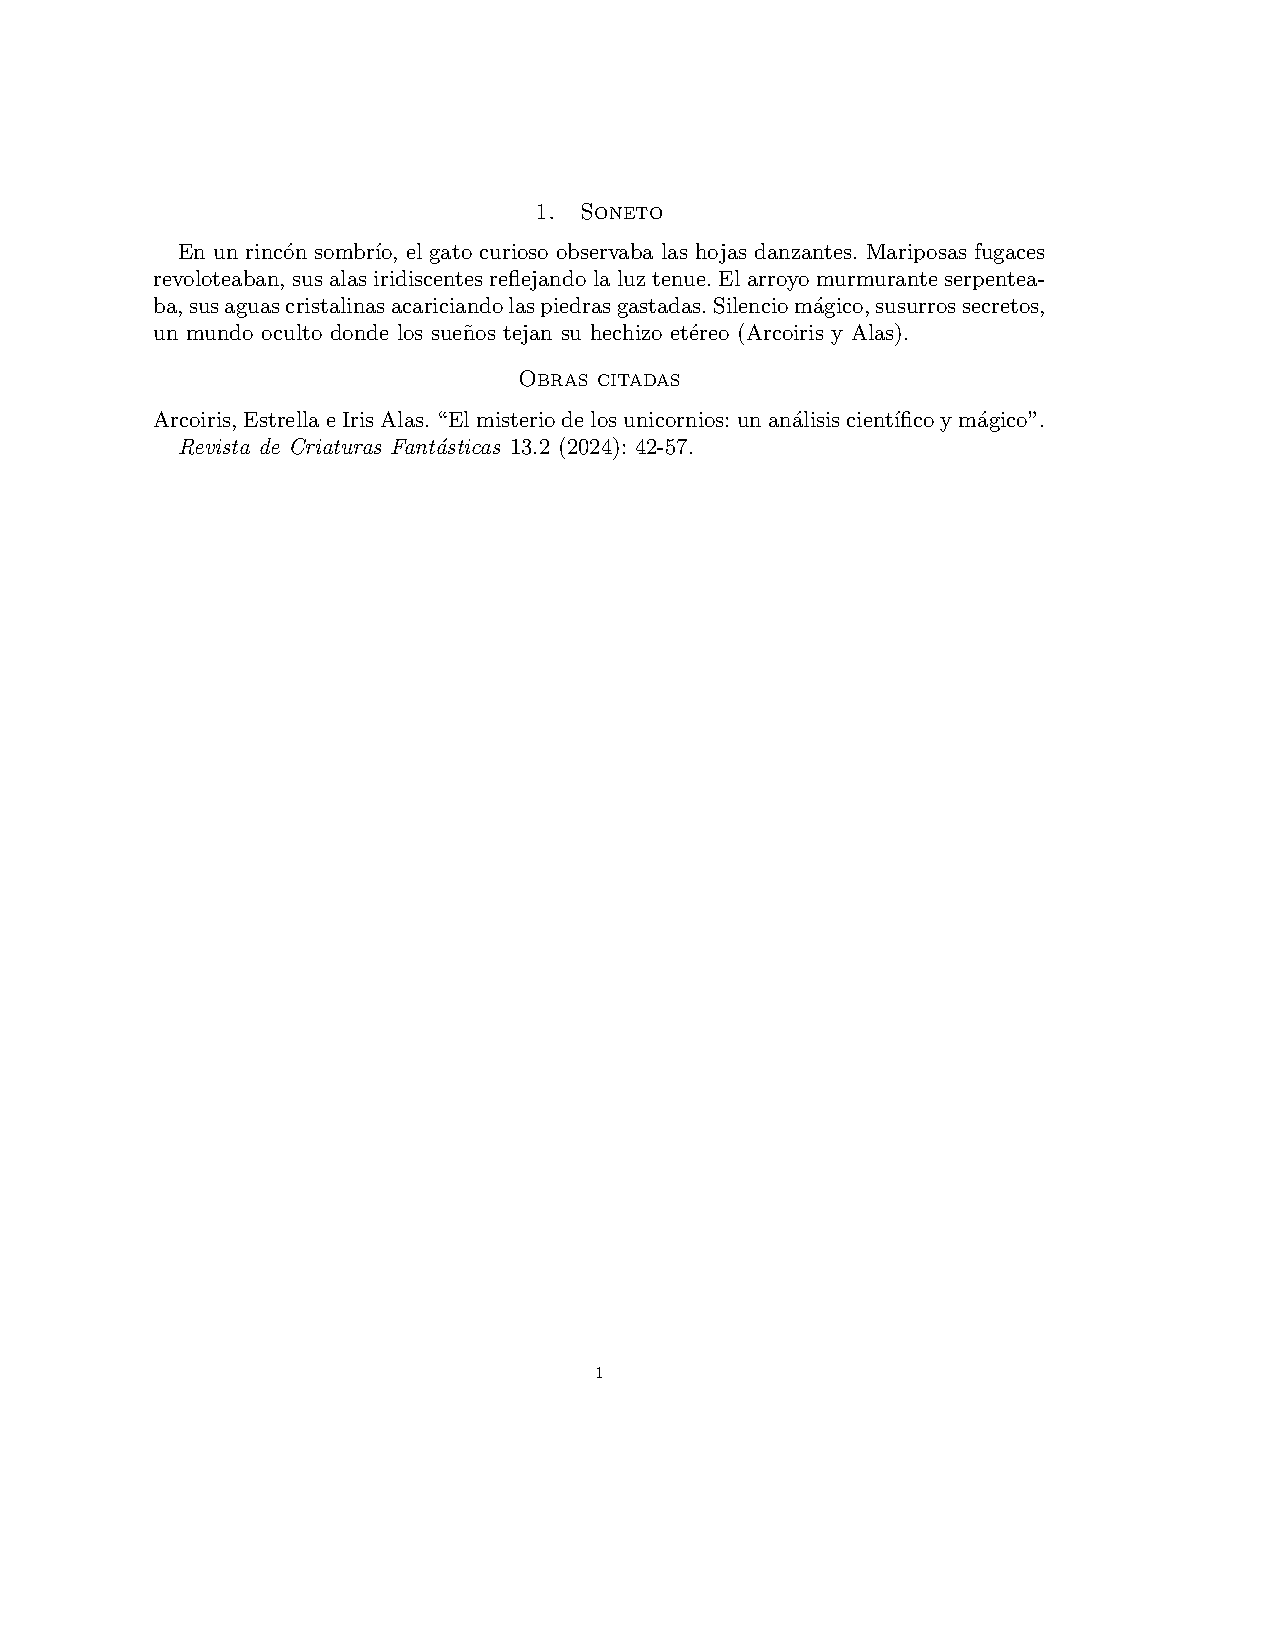
\includegraphics[scale=0.6, trim={2cm 20cm 3cm 3cm}, clip]{images/mla.pdf}
    \end{quote}
    \item Chicago: Este estilo tiene la posibilidad de formatear las citas de dos maneras diferentes: utilizando autor y fecha o con una nota al pie. Debe su nombre a la Universidad de Chicago donde fue creado y se emplea para citar en publicaciones científicas y académicas de distintos campos de humanidades, ciencias sociales y naturales. Un ejemplo de este formato es:
    \begin{quote}
        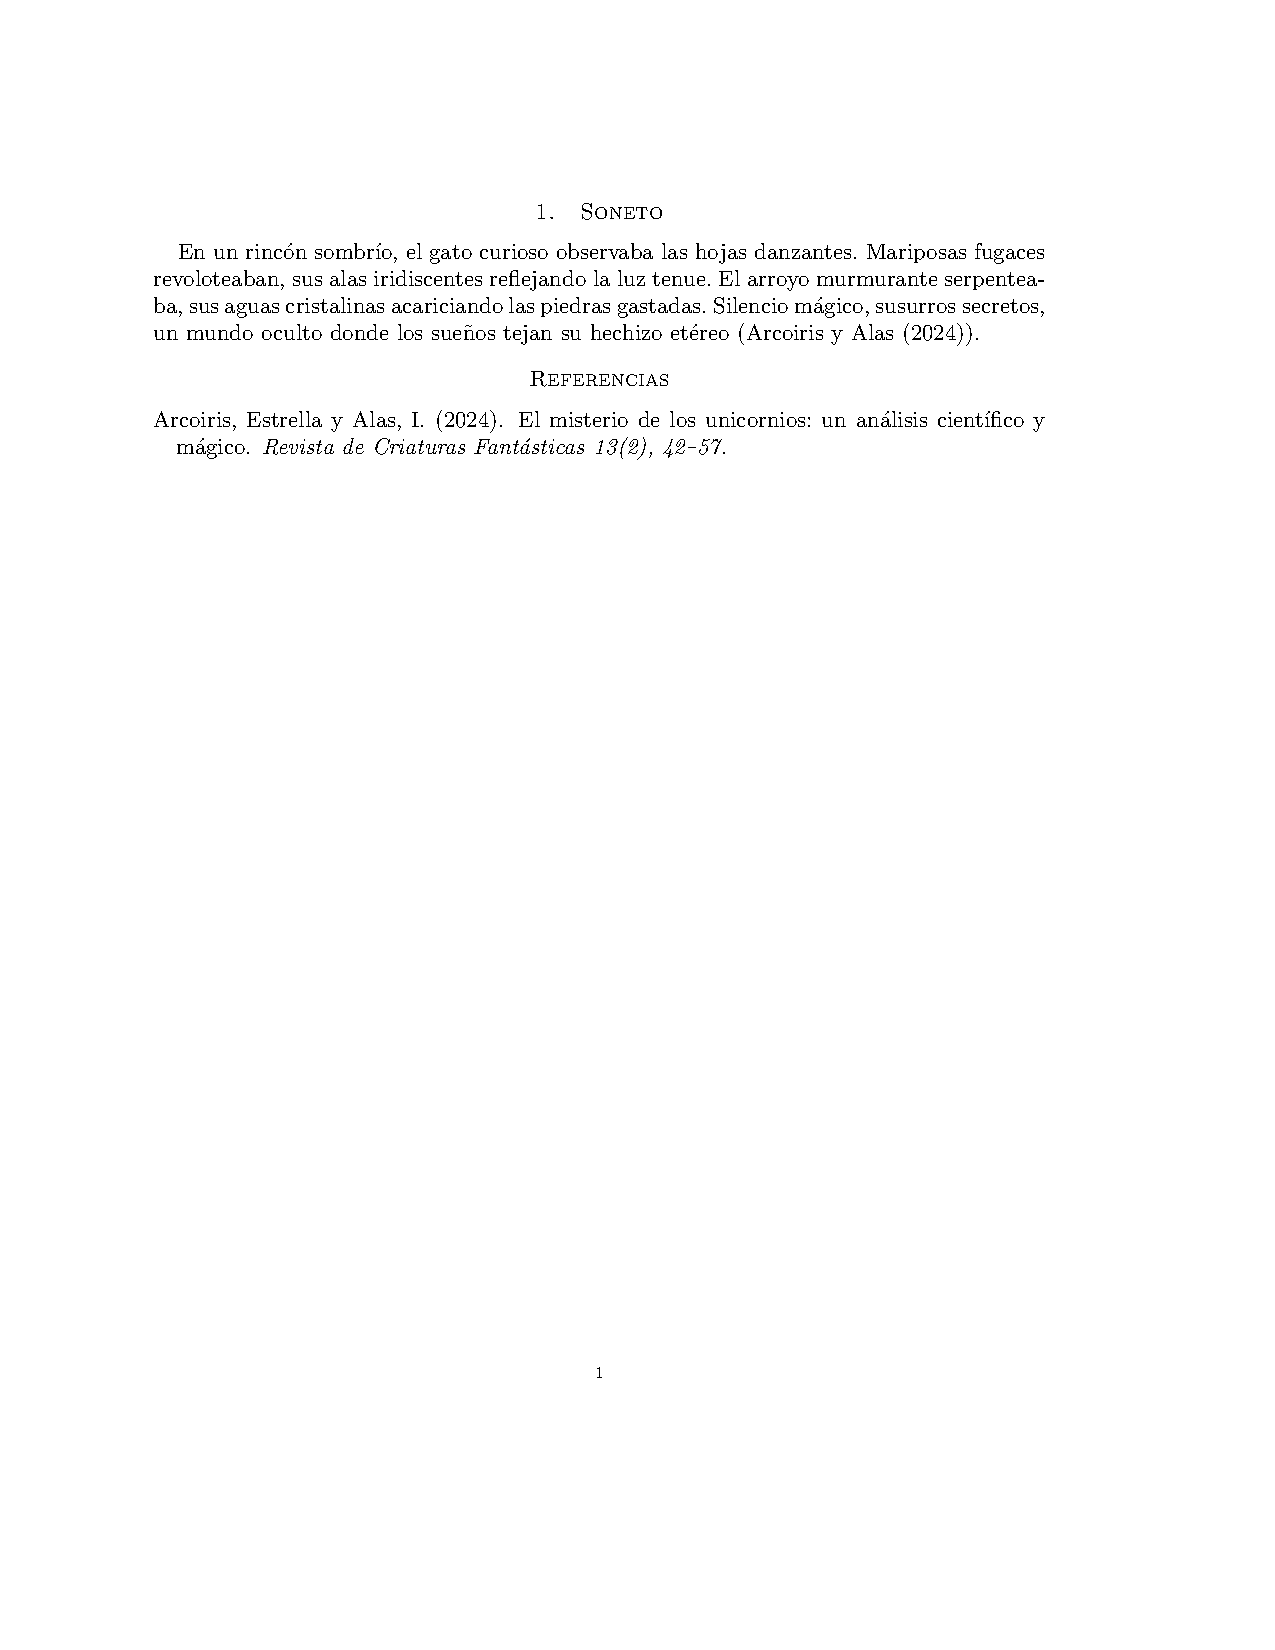
\includegraphics[scale=0.6, trim={2cm 20cm 3cm 3cm}, clip]{images/chicagoA.pdf}
    \end{quote}
    \item Harvard: Aunque este formato tiene su origen en la zoología y la biología en general, también es utilizado por los/las investigadores/as de distintas disciplinas como las ciencias sociales, la historia y las humanidades. Este sistema utiliza la información del autor-fecha para identificar una referencia bibliográfica. Un ejemplo de este formato es:
    \begin{quote}
        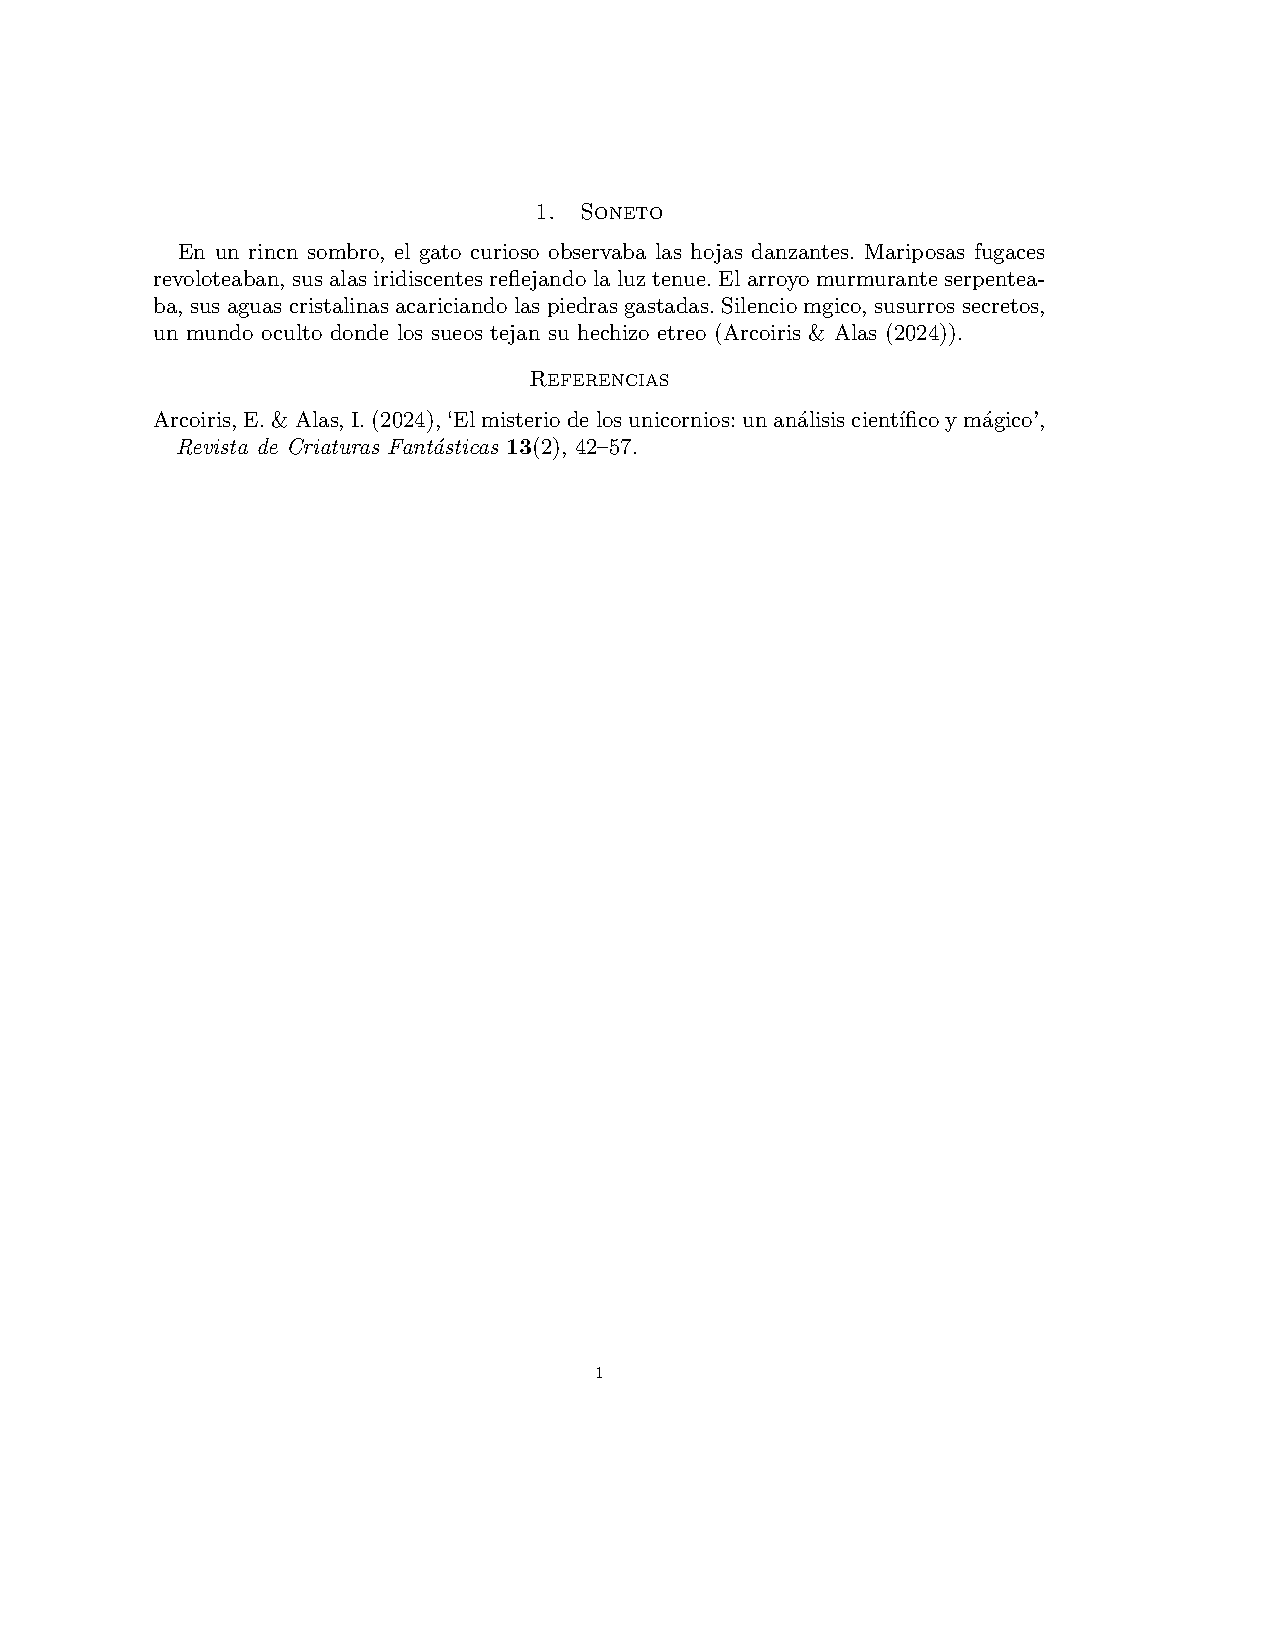
\includegraphics[scale=0.6, trim={2cm 20cm 3cm 3cm}, clip]{images/harvard.pdf}
    \end{quote}
    \item IEEE: En el estilo del Instituto de Ingenieros Eléctricos y Electrónicos (IEEE) las citas están numeradas entre corchetes. Toda la información bibliográfica se incluye exclusivamente en la lista de referencias al final del documento, junto al número de cita respectivo. Es el formato más utlizado en las ingenierías. Un ejemplo de este formato es:
    \begin{quote}
        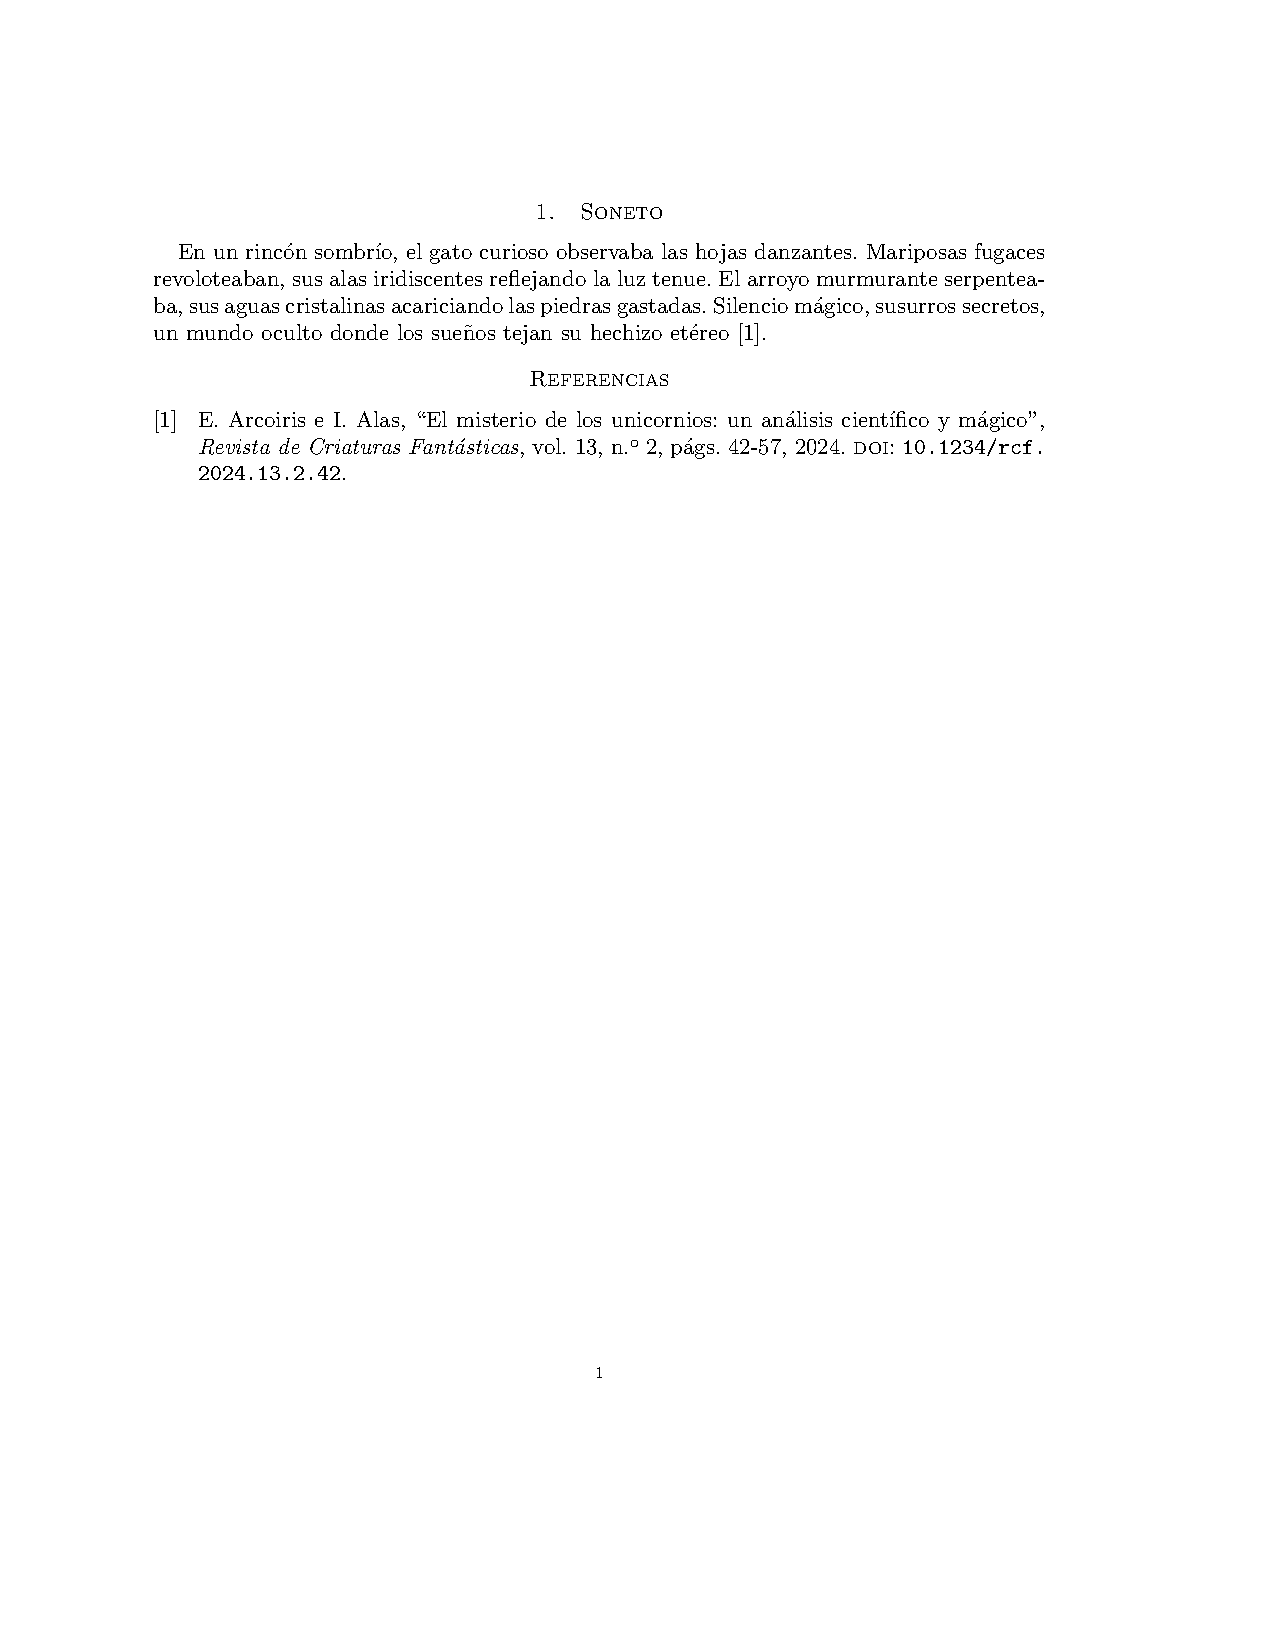
\includegraphics[scale=0.6, trim={2cm 19cm 3cm 3cm}, clip]{images/ieee.pdf}
    \end{quote}
\end{itemize}
\end{naranja}
Tienes libertad para elegir el estilo que más te guste, siempre y cuando utilices el mismo formato para toda la memoria. No puedes combinar distintos formatos en un solo documento.

\section{Herramientas de gestión de referencias y citas}

Organizar las citas y la bibliografía a mano no es nada recomendable. Imagina que cada vez que agregas una nueva cita tienes que ponerla en la bibliografía en la posición correcta y revisar que el formato sea el adecuado al estilo de citas que has elegido. Es por ello que existen muchas herramientas para poder tener las referencias controladas y accesibles. Dependiendo de que programa uses para escribir la memoria (e.g., Microsoft Word\texttrademark, \LaTeX\ u OpenOffice) tendrás disponibles unas u otras herramientas. La mayoría de los sistema de gestión de referencias y citas, sin embargo, suelen funcionar para cualquiera gracias a la posibilidad de importar y exportar las referencias en distintos formatos.

Los gestores de referencias y citas más populares son: EndNote (\url{https://endnote.com/es/}), Zotero (\url{https://www.zotero.org/}) y Mendeley (\url{https://www.mendeley.com/}). EndNote es una de las herramienta más completas y cómodas de usar, pero es una herramienta propietaria y es de pago. Mendeley es gratuita y te permite exportar conjuntos de bibliografías rápidamente. Zotero es la única de esta lista que es de código abierto. Existen muchas otras herramientas disponibles para descargar en Internet, con lo que te animo a explorar un poco más y elegir aquella que más cómoda te resulte. Verás la diferencia que hay entre utilizarla o tener que pasar horas poniendo las referencias y citas a mano.

En el caso de \LaTeX\ lo más apropiado es utilizar BibTeX. BibTeX es una herramienta y un formato de archivo para gestionar listas de referencias en documentos \LaTeX. Su función principal es generar automáticamente las citas y la lista de referencias en el formato seleccionado (e.g., APA, MLA, IEEE). También puedes utilizar herramientas independientes para la gestion de referencias y citas, como Mendeley, y combinarlas con \LaTeX\ y BibTeX.

\section{Consejos prácticos}

Como ya mencionamos, citar otras fuentes te permite respaldar tus argumentos. Es por ello que es imprescindible que utilices fuentes de información actualizadas, relevantes y confiables. Evita lo más posible citar la Wikipedia o Blogs de Internet no fiables. Intenta en su lugar cambiarlos por citas a libros o artículos científicos.

No utilices generadores automáticos de texto, como ChatGPT, para buscar referencias. Muchos de ellos no están conectados a Internet, e incluso los que lo hacen pueden inventarse las referencias. Debes mantener el rigor científico en las citas que selecciones para tu memoria.

No incluyas bibliografía que nunca cites en el texto. Si bien el sistema de BibTeX controla esto, no todos los gestores lo hacen. Recuerda revisar tu memoria una vez finalizada para detectar estos problemas antes de entregarla.

Es fundamental citar las fuentes que has utilizado en tu trabajo. Si no lo haces, tu texto podría considerarse plagio y acarrear consecuencias graves.

Mantén un registro organizado de las referencias usadas desde el comienzo de tu trabajo y actualiza la bibliografía a medida que avanzas en tu proyecto. No lo dejes para el último momento ya que es posible que llegado a ese punto te hayas olvidado de las fuentes de donde hayas sacado la información y tengas que perder el tiempo volviéndolas a buscar.

Por último recordarte que uno de los aspectos a valorar en el baremo de los trabajos fin de grado y máster incluyen un apartado relacionado con la búsqueda y tratamiento de la información. En particular se tiene en cuenta la calidad, cantidad y variedad de las fuentes, pero también su adecuación y fiabilidad. 
\include{11.anexostfg}
\chapter{La revisión del proyecto y la memoria}
\label{cap:Revisión}

% Comentarios:
% ¿Meter una lista de ítems a comprobar?
% ¿Aconsejar que se la confeccione el estudiante?
% Esto lo tendremos que ordenar por grupos.

Una vez que la memoria está terminada es el momento de comprobar que está correcta y que contiene todo lo que debe contener. ¿Por qué? Porque sencillamente se suele ir con prisas en esta parte final y es necesario revisarla para asegurarnos de que no nos falta nada. Para tal fin, te aconsejamos que hagas una lista de ítems ({\it checklist}) para comprobar y que determines si cumples con todos ellos. Nosotros te proponemos aquí algunas cosas que deberías chequear para que tú y tu tutor, añadáis lo que consideréis pertinente.


\begin{itemize}
  \item Sobre el formato de la memoria:

  \begin{todolist}
    \item Seguir la normativa de portadas (logos, colores, etc.) y prólogos (autorización, resumen, etc.).
    \item La portada contiene el título de TFG, el nombre autor y el de la persona que te tutoriza, así como la fecha de entrega o, al menos, el curso académico en el que se entrega.
    \item Los índices de contenidos para capítulos, secciones, tablas y figuras deben estar actualizados. Lo más sencillo es que los generes de forma automática.
    \item No quedan tablas cortadas al final de una página.
    \item Si hay títulos de secciones al final de una página, debajo de ellos debe haber al menos un párrafo.
    \item Utiliza los mismos estilos y tipo de letra en toda la memoria, a no ser que quieras resaltar algo como citas literales, fórmulas, ecuaciones o código.
    \item Todos los márgenes deben tener las mismas dimensiones, salvo casos excepcionales.
    \item Las páginas en blanco que dejes deben ser intencionales, por ejemplo, para que cada capítulo empiece en página impar.
    \item Las páginas están numeradas (correctamente).
 \end{todolist}

  \item Sobre la estructura:
  \begin{todolist}
    \item Están todas las secciones que, según el tipo de TFG, deben aparecer. 
    \item El resumen claramente describe de forma concisa qué se ha realizado en el TFG.
    \item La introducción establece claramente el contexto y la motivación necesarias para entender el problema entre manos.
    \item Están los objetivos. Son claros y concisos.
    \item Están las conclusiones, donde se muestran los resultados y contribuciones del TFG, y los trabajos futuros.
    \item Está la bibliografía.
    \item Están todos los anexos necesarios.
    \item Es interesante incluir un anexo con el glosario de términos y abreviaturas empleados en la memoria.
  \end{todolist}
  
  \item Sobre la bibliografía:

  \begin{todolist}
    \item Todas las referencias de la bibliografía deberían aparecer citadas en el texto.
    \item Todas las citas bibliográficas del texto deben tener una referencia asociada.
    \item Las referencias bibliográficas deben estar completas y también todas en el mismo formato.
    \item Las referencias de recursos de Internet deben indicar también la fecha de la última consulta.
  \end{todolist}

  \item Sobre las figuras y tablas:

  \begin{todolist}
    \item Todas las figuras y tablas deben estar numeradas secuencialmente y referenciadas/citadas en el texto.
    \item Todas las figuras y tablas deben tener un título descriptivo ({\it{caption}}).
    \item Los títulos de figuras y tablas deben estar en la misma página de la figura o tabla.
    \item Si se usan figuras hechas por otra persona deberían ser citadas/usadas correctamente, por ejemplo en el pie de figura ``Extraído de [x]'' o ``Fuente: [x]'', si no, indicar ``Elaboración propia''.
    \item Las imágenes y las tablas están dentro del espacio del cuerpo de la página y ninguna se desborda hacia los márgenes. 
  \end{todolist}

  \item Y por último:

  \begin{todolist}
    \item Uso de un lenguaje adecuado y 
    \item que no haya errores ortográficos ni gramaticales, por lo que más quieras (¡¡¡Pásale el corrector ortográfico, por favor!!!).
  \end{todolist}

\end{itemize}

Además, también te recomendamos que te descargues las rúbricas de evaluación del tutor y de la comisión y compruebes que tratas, de una u otra forma, todos los puntos que aparecen en ella. Esto es importante porque si te dejas alguno sin tratar, los miembros de la comisión pueden preguntarte por él. Quien evita la ocasión, evita el peligro ;-)
\chapter{La elaboración de la presentación en la defensa} \label{cap:elaboraciónPresentación}

% [Autores: Pablo, Alberto]

¡Ya queda menos para poder presentar el proyecto! Has llegado a los objetivos que te habías propuesto (tu programa ya funciona, tus resultados experimentales son geniales...), has entregado la memoria en tiempo y forma y ya estás listo para enseñar tus avances al mundo.

Después de todo el esfuerzo, de todas las horas, de todos los cabezazos contra la pantalla, resulta que solo tienes 20-25 minutos ante un tribunal para contarles lo que has hecho. Además, seamos sinceros, muchas veces el tribunal se va a leer la memoria de pasada mientras estas haciendo la presentación, así que te juegas mucho dependiendo de cómo lo hagas en esos 20 minutos y lo que enseñes y no enseñes. En este capítulo te enseñaremos cómo preparar la presentación, es decir el archivo (el PDF, el ODP, el PPTX) que proyectarás en el aula, mientras que en el siguiente capítulo nos centraremos en cómo preparar la defensa de esa presentación.

\section{Centrarte en lo importante}

El primer consejo que te vamos a dar es que el tribunal tiene que mirarte a ti, no a las diapositivas. Tú eres la estrella de la función, y la presentación es un apoyo a lo que estás diciendo. El segundo consejo, y más importante todavía, es: \textbf{no te pases del tiempo}. Alguien del tribunal tiene un cronómetro encendido y no hay nada que quede peor en una defensa que decirle al estudiante ``lo siento, tienes que cortar''. Así que no prepares 50 diapositivas y quieras contarlo todo con miles de pelos y señales. Por ejemplo, entre otras muchas cosas, puedes ahorrarte diapositivas de bibliografía, que aportan poco en la defensa.

Aunque dependerá del tipo de TFG que realices, una posible estructura puede ser la siguiente:
\begin{itemize}
\item Título del proyecto, fecha, tu nombre y tu correo electrónico y el nombre de tu director o directora. Logos de la universidad y escuela, para dejarlo más profesional.
\item La segunda diapositiva debe ser un índice numerado de las secciones de la presentación.
\item Una o dos diapositivas de introducción y contexto.
\item Una diapositiva definiendo los objetivos.
\item Una diapositiva resumiendo el estado del arte.
\item Una o dos diapositivas de planificación y metodología.
\item Si tu trabajo es de desarrollo:
    \begin{itemize}
    \item Dos o tres diapositivas del diseño e implementación, diagramas sobre todo.
    \item Una diapositiva hablando de pruebas.
    \item Capturas de la UI, aunque mejor haz una demo.
    \end{itemize}
\item Si tu trabajo es experimentación o investigación:
    \begin{itemize}
        \item Dos o tres diapositivas describiendo el método y mostrando los resultados (gráficas sobre todo). Dependiendo del número de experimentos que realices quizás necesites más. Pero recuerda, casi siempre menos es más.
    \end{itemize}
\item Una diapositiva de conclusiones, incluyendo enlace a repositorio del código, si lo hubiera.
\item Una diapositiva de despedida, con un texto parecido a ``Muchas gracias por su atención''.
\end{itemize}

Esto nos lleva a una presentación con 15 a 20 diapositivas aproximadamente. Si te centras un minuto en cada una, y créenos, un minuto pasa muy rápido, ya lo tienes listo.

Respecto a los títulos de las diapositivas, mucha gente cambia el título de cada una para que sea como un titular de periódico, que le da un toque más innovador.  Es decir, en vez de poner títulos genéricos como ``Introducción (I)'' o ``Introducción (II)'' puedes poner una diapositiva (que no usaremos en el conteo) con el texto centrado ``Introducción'' y pasar rápidamente a las siguientes tituladas ``El problema de los tres cuerpos es muy difícil de resolver'' y ``Se han utilizado algunas cosas sin éxito''. Fíjate como parecen titulares de periódico, pero seguimos siendo conscientes de que estamos en la introducción. De hecho, como curiosidad, fíjate también en los nombres de las secciones de este capítulo, no hace falta leer el texto para sacar la idea principal de cada una. De esta forma, estamos ofreciendo una especie de idea principal del contenido de la diapositiva que el espectador agradecerá enormemente.

\section{La presentación no es un karaoke}

Si vas a leer lo que pone en las diapositivas envíala por correo y nos ahorramos tiempo. Y recuerda que menos es más. Así que quita la broza. En tu memoria quizás hayas escrito algo como 

``\textit{El objetivo de este proyecto es demostrar que, bajo ciertas condiciones, utilizar el algoritmo Williamsito, creado por Williams [11] permite obtener mejor rendimiento para resolver el problema de los tres cuerpos [12] reduciendo el tiempo de computación}''. 

Pues eso, en la presentación quita la broza: 

``\textit{Williamsito reduce el tiempo para resolver el problema de los tres cuerpos}''. 

Ya está, dicen exactamente lo mismo, pero más rápido. El tribunal lo habrá pillado enseguida y podemos pasar a otra cosa.

Especialmente importante será la diapositiva de conclusiones. Es la última carta que tienes en la manga para que el tribunal vea que has hecho un buen trabajo.

\section{El poder de lo visual}
Vamos a mejorar el texto anterior: 

``\textit{Williamsito \textbf{reduce el tiempo} para resolver el problema de los tres cuerpos}''. 

Fíjate cómo hemos usado un componente visual (la negrita) para ir directamente a la idea de la frase. No te cortes en usar técnicas tipográficas para facilitar la lectura (negrita, cursiva, color), pero tampoco te pases. Resaltar de una a tres palabras por frase es más que suficiente. Piensa que lo que no haya que resaltar quizá es que directamente no debería estar en la diapositiva...

A veces incluso se puede sustituir el texto con una imagen o un pictograma que represente la idea. Por ejemplo, en vez de poner una lista de los componentes de tu sistema y lo que hacen, utiliza un diagrama. De un solo vistazo vemos que tiene 5 componentes y se comunican usando MQTT. Perfecto, todo claro. 

Pero igual que antes, no pongas diagramas que no aporten y te pongas a explicarlos. El diagrama de clases o el de E/R, por ejemplo, generalmente no aportan absolutamente nada en la presentación, ya has aprobado las asignaturas que te lo evaluaban. Tampoco pongas código fuente, a menos que sea realmente necesario.

Y ojo con los colores. Utiliza paletas ya establecidas. Existen webs que te permiten coger un grupo de 4 colores que combinan bien. Por ejemplo Coolors.co \footnote{\url{https://coolors.co}}, pero hay otras muchas. A menos que sepas de diseño gráfico y teoría del color no te fíes de tu criterio artístico. Esto es especialmente importante si estás visualizando datos. Además, puede haber personas daltónicas en el tribunal.

Además, texto oscuro en fondo claro hace que el público mire a la diapositiva, pero texto claro sobre fondo oscuro hace que miren al orador.

Y para terminar un consejo muy fácil de aplicar y que queda muy bien: añade el número de diapositiva actual y el total de diapositivas en una esquina (Por ejemplo, \textit{4 de 20}). De este modo el tribunal podrá orientarse y saber cuánto te queda o anotar la diapositiva sobre la que hacerte una pregunta. Si, por ejemplo, ven que te pasas un poco de tiempo pero solo te queda una diapositiva quizás no te interrumpan. También servirá para que en el turno de preguntas puedas moverte a una diapositiva concreta si te lo piden.

\subsection{Memes y gifs}

Actualmente, aunque pueda resultar poco ortodoxo, hemos acumulado una gran cantidad de información a través de memes y gifs. Si encuentras uno que se ajuste a lo que quieres decir, no dudes en incluirlo en tu presentación. Eso sí, no abuses de ellos, ya que pueden hacer que tu presentación parezca poco seria y considera que el salto generacional entre el tribunal y tú puede hacer que no entiendan la referencia. 

\section{Show. Don't tell.}

Esto es un aforismo que se usa mucho en el guión cinematográfico. En vez de escribir qué hace tu aplicación prepara una demo de dos o tres minutos en la que veamos cómo funciona. No hace falta que muestres todo, por ejemplo, como crear usuarios, que es algo trivial, sino la parte interesante.

Si tienes miedo de que algo falle (por ejemplo, si el servidor está en tu casa), prepara un vídeo, pero no grabes tu voz explicándolo, da la explicación en directo mientras que visualizas el vídeo. En el turno de preguntas puedes ofrecer al tribunal probar la aplicación o hacer la demo en vivo para evitar sospechas y actos de fe sobre el trabajo mostrado en el vídeo.

Consensúa esta presentación con la persona que te tutoriza el TFG hasta que estéis ambos contentos con ella. Confía en su criterio, ya que ha visto muchas presentaciones pero recuerda que eres tú el que va a hacer la presentación así que procura estar cómodo con ella aunque no sigas todos los consejos que te hemos dado o te ha comentado el tutor.



\chapter{La defensa}
\label{cap:Defensa}
% [Autores: Juanma, Alberto]

\section{La estructura del acto}

Una vez que finalice el periodo de entrega del TFG, el centro publicará las comisiones de evaluación y los TFGs asignados a cada una. La comisión está compuesta de tres miembros. A saber: un presidente, un secretario y un vocal. Una vez nombrada, el presidente, normalmente, convocará a los estudiantes, informándoles de la fecha, hora y lugar del acto de defensa, Este se divide, como bien hemos indicado anteriormente, en dos fases: la presentación del trabajo y la discusión con los miembros de la comisión.

El acto es público por lo que puedes entrar a ver a tus compañeros. El que lo hagas o no dependerá de ti, de si te pones nervioso viendo a otros o no o de si quieres estar tranquilo y concentrado antes. Si te quedas fuera de la sala, quédate cerca de ella. El secretario saldrá a llamarte cuando sea tu turno. En ese momento, entras en la sala, saludas al tribunal (buenos días, buenas tardes, hola) y te diriges al lugar donde expondrás, conectas tu portátil al proyector y preparas la presentación. 

El presidente, en ese momento, dirá algo así como que se va a dar comienzo a la defensa del TFG titulado X realizado por el estudiante Y. Y te informará de la estructura del acto, indicándote explícitamente el tiempo que tienes disponible para la exposición (normalmente veinte minutos) y el tiempo, aproximado éste, de la ronda de preguntas y comentarios (otros veinte minutos habitualmente). Tras la presentación, que comenzarás sólo cuando el presidente te dé la palabra, éste dará paso al secretario y al vocal, los cuales te plantearán sus cuestiones, participando finalmente el propio presidente en dicha ronda. Una vez finalizada la segunda fase, éste te dirá que se ha concluido el acto, te dirá que se te comunicará la nota en uno o dos días y, finalmente, te dará las gracias. Lo habitual es que tú también des las gracias. Y... se acabó lo que se daba. Ya has terminado, recoges y abandonas la sala o bien te quedas a oír a los compañeros siguientes.

Como ya hemos indicado, es un acto público por lo que también pueden asistir tus familiares y amigos. El que lo hagan o no, dependerá también de ti: si tus padres y hermanos o amigos quieren ir a verte y tú no te pones nervioso con su presencia, es un momento bonito para que te vean en acción y lo compartan contigo. A veces te puedes sentir más tranquilo con su presencia. Si no es así, mejor les dices que prefieres que no vayan y no hay ningún problema. De cualquier forma, el público en general y los familiares y amigos en particular, deben permanecer en silencio, sin intervenir en ningún momento y sin realizar comentarios de ningún tipo a las preguntas de la comisión ni a tus respuestas. Tampoco es normal que se aplauda cuando finalices. Los abrazos y felicitaciones déjalos para cuando estés fuera de la sala.

\section{La importancia de la defensa}

%https://www.youtube.com/watch?v=AK_xGgGSdCo

Una vez entregado el TFG, la siguiente y última fase en el proceso es la defensa de tu trabajo. Es conveniente que descanses y desconectes uno o dos días antes de ponerte a trabajar en la confección del material que usarás en la defensa. Te permitirá hacer esas tareas mucho más tranquilamente, con más concentración y ganas. Has trabajado muy duro durante todo el curso y en especial en las últimas semanas previas a la entrega y el cansancio y el estrés se acumulan. Y es oportuno hacerlo porque este acto es el momento de la verdad donde tu TFG será evaluado y tienes que estar fresco/a y en plenitud de condiciones.

La defensa, y su preparación, tienes que tomártela en serio. Es el principal acto académico que vas a realizar en tus estudios y de su resultado dependerá la nota de tu proyecto. Tu trabajo ya está terminado y en este acto lo que tienes que hacer es convencer a los miembros de la comisión de que es un buen trabajo. Puedes haber realizado un trabajo excepcional pero si no lo "vendes" bien, la nota que tengas no será la que verdaderamente refleje la calidad de tu TFG (y esto es un hecho que, lamentablemente ocurre muy frecuentemente). Imagínate que eres un vendedor de motos y tienes la mejor del mercado. La moto no se vende por sí sola, tienes que hacerle ver al cliente todas las magníficas prestaciones que hacen que sea una de las mejores del mercado, si no la mejor, y conseguir que la compre. Si no lo haces así el cliente no se va a enterar ni vas a poder "venderle la moto". Por tanto, tan importante es elaborar un buen TFG, tanto el producto como la memoria, como comunicarlo a los miembros de la comisión. 

Pero ojo, "vender la moto" no es "vender humo". Una cosa es que emplees todas las técnicas de comunicación a tu alcance para mostrar la calidad del producto y el trabajo desarrollado, y otra es que las utilices para tratar de engañar a la comisión, exagerando o engordando tu trabajo. Ten cuidado porque estas cosas son muy fáciles de detectar y te pueden poner en un aprieto, sobre todo porque los miembros de la comisión han leído tu memoria y saben lo que has hecho y además disponen de un informe del tutor sobre tu trabajo.

Por tanto, tu capacidad de comunicación jugará un papel importante en esta fase. Mediante una comunicación efectiva serás capaz de expresar de forma clara, concisa y efectiva, tus ideas, facilitando su comprensión por parte de la comisión. Las habilidades de comunicación podemos dividirlas en dos: la verbal y la no verbal. La primera implica al lenguaje hablado (uso de vocabulario, gramática, volumen y tono de voz); la segunda, tiene que ver con la forma de comunicar sin hablar, es decir, la parte más física: las posturas, gestos, miradas, etc. Estos dos tipos los describiremos con más profundidad en la siguiente sección pero sé consciente que ambos son importantes en la defensa. Esta comunicación la apoyarás en una presentación clara y concisa y bien estructurada, como se ha indicado en el capítulo anterior, en la fase de exposición de tu trabajo, pero también tendrás que hacerlo sin apoyo en la fase de discusión con la comisión, donde te realizarán preguntas y comentarios sobre tu trabajo y tendrás que responder de forma clara, concisa y convincente.

Por tanto, si comunicas de forma efectiva, no vas a tener problema en hacer ver el trabajo que has realizado y, por tanto, la comisión será capaz de entender lo bueno que es. 

Algunos consejos para preparar la defensa son los siguientes:

\begin{itemize}

    \item Prepara la defensa con la persona que te tutoriza. Esto es un proceso iterativo donde inicialmente te indicará las líneas generales con las que debes hacer la presentación. Seguidamente, prepara un primer borrador y se lo pasas al docente para que lo evalúe. Te hará los comentarios pertinentes. Si tienes dudas sobre ellos, habla con él y llega a acuerdos. Refléjalos en la presentación y vuelve a enviárselos. Este proceso se repetirá hasta que haya una estabilidad en la presentación y no haya cambios. En ese momento puedes decir que tienes lista la presentación y puedes comenzar a ensayar.

    \item No sólo prepara una presentación sino también una demostración, si el tipo de TFG que has desarrollado se presta a esto. Puedes hacer un vídeo mostrando las prestaciones de tu software o una demostración en vivo del mismo. De cualquier forma, acuerda con la persona que te tutoriza lo más relevante de esta demostración y el tiempo que le vas a dedicar, el momento en lo harás y prepárala concienzudamente también. 

    \item Normalmente afrontamos este acto con inseguridad y miedo. Para evitarlo, la única receta que hay es ensayar la presentación una y otra vez hasta que tengas seguridad y confianza y sepas qué decir en cada momento. También imagínate cómo va a ser la defensa, la sala, los miembros, dónde estarás tú situado, los gestos que harás, cómo te moverás. Este entrenamiento te dará confianza en ti mismo.

    \item Cronométrate en los ensayos. No puedes pasarte del tiempo indicado para la exposición. Si lo haces, el presidente te podrá decir que te has excedido del tiempo asignado y retirarte la palabra. Esto implica que puede haber cosas importantes que te dejes sin comentar, con el consiguiente problema para que los docentes que te evalúen comprendan la dimensión, dificultad, alcance, etc. de tu trabajo. Además, aunque te dejaran más tiempo, dejarías mala impresión en los miembros de la comisión y hay un item de la rúbrica que evalúa esto. Por tanto, cronométrate y ajústate al tiempo. Esto puede implicar que elimines diapositivas, que las hagas más breves, que contengan menos texto, que simplemente pases por encima de algunas diciendo apenas una frase. Cualquier cosa para ajustarte al tiempo pero, ojo, sin que el mensaje pierda contenido importante.

    \item Piensa en posibles preguntas que los miembros de la comisión podrían hacerte y prepara las respuestas. Estas suelen ser del tipo:

    \begin{itemize}
        \item ¿Por qué has hecho esto de esa forma?
        \item ¿Por qué no has tenido en cuenta esto?
        \item ¿Cuáles son las limitaciones de tu trabajo?
        \item ¿Qué aporta tu trabajo?
        \item ¿Por qué has elegido esta opción y no esta otra?
        \item ¿Por qué no has liberado tu código? 
        \item ¿Por qué has escogido esta licencia y no otra?
        \item ¿Por qué no has incluido X en tu revisión del estado del arte?
        \item ¿Por qué no has mencionado ni valorado el uso de esta tecnología, metodología, método o herramienta?
        \item ¿Cómo abordarías la propuesta X de tus trabajos futuros? 
        \item [PONER MÁS PREGUNTAS TIPO]
    \end{itemize}

    \item Como ya se ha explicado en el capítulo anterior, la presentación es un mero elemento de apoyo para presentar tu proyecto. Es un guión para que tú sepas qué tienes que decir. Por tanto, no leas su contenido. Y para que puedas decir todo lo que debes decir, cuando diseñes la presentación hazte un documento donde escribas las cosas que tienes que comunicar en cada diapositiva y apréndetelo. Pero en la exposición no hables como un loro que suelta el texto de memoria, ve con tranquilidad, haciendo pausas y dirigiéndote a los miembros de la comisión y explica las cosas. No las recites. Lo de aprenderse todo lo que tienes que decir es para evitar dejarte algo que sea importante. 

    \item Practica la exposición con la persona que te tutoriza, si es posible. Él o ella te indicarán aspectos a mejorar de la presentación y de la comunicación. Además podréis simular el turno de preguntas y te hará algunas que son habituales en las comisiones y otras específicas que pueden surgir tras exponer la presentación. Y, sabiendo de antemano quiénes serán los examinadores, también te podrá indicar algunas típicas de estos profesores. También te hará comentarios sobre las respuestas que das, tanto en forma como en contenido.

    \item Practica la exposición con tus familiares y amigos. Ellos no van a entender la parte técnica, pero sí que te podrán dar una realimentación muy valiosa sobre la forma de expresarte, moverte, gestos, muletillas o cualquier otra cosa que les llame la atención. Haz caso a sus comentarios y ensaya de nuevo, ya sin ellos, procurando evitar las situaciones negativas que te han indicado. Si no tienes posibilidad de tener espectadores en los ensayos, grábate tú con el móvil y luego analiza minuciosamente toda la exposición para ver qué cosas tienes que mejorar.

    \item Si es posible, por las fechas y horarios, asiste a alguna otra defensa. De esta manera podrás ver en directo todo el proceso, la exposición que hace el estudiante, las preguntas y cómo responde. Esto te servirá para entender el acto y para quitarte el miedo, pues es una situación que, aunque importante y algo más relevante, ya habrás realizado en múltiples ocasiones en tu grado.

    \item Procura preparar la presentación, llevar a cabo las correspondientes modificaciones, y los ensayos pertinentes con tiempo, de tal manera que no necesites nada más que dar un pequeño repaso a la misma el día anterior de tu defensa. Estarás más tranquilo/a ya que llegar al día de antes sin tenerla bien preparada sólo es una fuente de nervios y tensión que te perjudicará. Ese día descansa y come especialmente bien. 
    
\end{itemize}

Y algunos otros para el momento de la defensa:

\begin{itemize}
    \item Imaginamos que en el momento de comenzar tendrás nervios. Eso es normal. No te preocupes. Siempre es mejor tener un poco de tensión que ir súper relajado. Esos nervios se irán disipando conforme avances. Al comenzar, respira hondo y empieza con tu exposición. Céntrate en contar qué y cómo has hecho de una manera lo más efectiva posible.

    \item Ha sido periodo largo de trabajo duro y ahora llega el momento que lo culmina. Nadie sabe más que tú del trabajo que has hecho, del cual debes sentirte orgulloso/s, cosa que debe infundirte seguridad, por tanto, disfruta de la presentación. 

    \item Intenta captar continuamente la atención de los miembros de la comisión empleando tanto un buen diseño de las diapositivas, tal y como se ha explicado en el Capítulo \ref{elaboración_presentacion}, como técnicas verbales, como, por ejemplo, usando preguntas que lanzas a la comisión, pero que no esperas que respondan, cambios de volumen y tono, etc.

    \item Llévate un guión que será de ayuda si en algún momento te quedas en blanco o no te acuerdas por dónde seguir, pero no lo tengas en la mano. Déjalo en la mesa a un lado.

    \item Si los miembros del tribunal no te están mostrando en algún momento atención, no te preocupes. No significa que no le interese tu presentación ni que hayan dejado de escucharte. Simplemente estarán mirando algo en la memoria o anotando alguna cuestión a hacerte. Tú no te pongas nervioso/a ni pienses que no les está gustando tu presentación y sigue con ella, mirándolos como si ellos te estuvieran mirando y escuchando también.

    \item Tanto en la presentación como en la respuestas sé claro y ve al grano. No hay mucho tiempo y si te vas por las ramas te vas a quedar sin tiempo para explicar cosas importantes. Y sé honesto y sincero. Si algo no lo has hecho, por ejemplo, y te preguntan, di que no lo has hecho y el porqué. No te inventes nada porque los miembros de la comisión se darán cuenta y te meterás en un lío.

    \item Pon en móvil en modo avión y no lo sitúes a la vista. La única excepción a esto último es que lo quieras emplear como temporizador para ver el tiempo de exposición, aunque si la tienes bien ensayada, tampoco es necesario el móvil y ofreces una mejor imagen que si estás consultándolo continuamente para ver cuánto tiempo te queda.
\end{itemize}

En la referencia \cite{vallejo2009defensa} y tienes algunos otros consejos que te podrán ser útiles en este acto de la defensa.


\section{La comunicación con la comisión}

La forma de interactuar con los miembros de la comisión es también muy importante en el acto de la defensa. En esta sección te hacemos varias recomendaciones sobre este asunto.

Si el presidente de la comisión no te ha presentado, entonces tras darte la palabra, y tu agradecerla, preséntate tú mismo e indica seguidamente que vas a presentar tu trabajo fin de grado, con el título correspondiente. Si ya te ha presentado, entonces da las gracias y di que comienzas con la presentación de tu TFG (y no vuelvas a presentarte). 

Cuando finalices tu presentación, puedes decir algo así como "y con esto finalizo la presentación de este TFG y quedo a disposición de la comisión para resolver cualquier duda o comentario que deseen realizar", y esperas a que tome la palabra el presidente para organizar la segunda fase del acto. En ese momento comenzará la ronda de preguntas. 

Lo habitual es dirigirse a los miembros de la comisión de usted y siempre con el máximo respeto. Invócalos mediante la denominación de profesor y su apellido
(profesora García). Seguramente conoces a los docentes que estén en la comisión. Alguno te habrá dado clase en alguna asignatura del grado y tienes cierta confianza. En ese caso, puedes bajar algo el nivel de formalidad a la hora de dirigirte a ellos aunque nunca entrando en el colegueo. En ese caso puedes llamarlos por su nombre de pila. Si el presidente te habla de Usted, lo normal es que hables tú también en ese grado. Si lo hace de tú, decide si hablarles también de tú o de Usted. 

En relación a las preguntas y comentarios, como ya hemos indicado anteriormente, responde siempre yendo al grano y de forma clara. No des rodeos ni respondas otra cosa si no sabes qué decir o no quieres decir algo. Habla con sinceridad. Si no entiendes una pregunta di que no has comprendido qué quieren decirte y que, por favor, te la repitan. Si no estás de acuerdo con algún comentario, siempre con educación y de forma cortés, rebátelo y ofrece las razones por las que discrepas. No tengas miedo a hacerlo así. Eso es una discusión académica y es un punto a tu favor, ya que estás dejando claro a la comisión que tienes los conocimientos y la capacidad para defender lo que has hecho y el porqué.

Sé receptivo/a a los comentarios, críticas y sugerencias. No te los tomes a mal. En algunas situaciones puedes responder que gracias por el comentario y que lo tendrás en cuenta para mejorar la aplicación, por ejemplo. 

No tengas miedo de preguntar cualquier cuestión o pedirles ayuda en algún tema (por ejemplo, si al conectar el ordenador al proyector hay algún problema). Los docentes de la comisión te responderán con toda amabilidad y te ayudarán en la medida de sus posibilidades. También son conscientes de que se pasan algunos nervios en este tipo de actos y, por tanto, serán comprensivos y te intentarán tranquilizar.

Ten también presente que los miembros del tribunal no van a preguntarte con mala intención, simplemente están haciendo su trabajo y deben plantear ciertas cuestiones para entender detalles que no les han quedado claros o conocer tu capacidad para desenvolverte en estas situaciones. En definitiva, tienen que tener toda la información disponible para poder evaluar objetivamente tu trabajo.

\section{Cuestiones de protocolo}

La principal cuestión en este apartado es la vestimenta. ¿Qué me pongo? ¿Voy muy arreglado? ¿Voy como normalmente visto? La respuesta es sencilla pero a la vez complicada: irás vestido de la forma adecuada para ofrecer la imagen que quieres dar. Por lo pronto, no irás vestido como vas a clase, a una boda, o como sales con los amigos (evita camisetas, tirantes, bermudas, pantalones cortos o ropa deportiva), ya que es un atuendo demasiado informal para una presentación pública de este calibre. ¿Irías como vistes normalmente a una entrevista de trabajo? No, ¿verdad? Pues esa es la idea en este acto. 

Uno de los aspectos que da más información sobre ti es tu forma de vestir ya que refleja tu personalidad y esta también permite a los demás construir una primera impresión sobre ti en muy poco tiempo. Y lo que quieres es caer bien a los miembros de la comisión y que se lleven una primera impresión de que eres un profesional.

En general, simplemente debes ir vestido acorde al acto en el que vas a participar. Si fuera el de defensa de una tesis doctoral, claramente deberías ir de traje pero esta presentación pública, aunque importante, podríamos decir que no tiene la categoría de la defensa de un trabajo doctoral. Por tanto, debes ir arreglado pero no es necesario súper arreglado. Un pantalón de vestir y una camisa podrían ser suficientes. Evalúa también una falda y una blusa o camisa, o un vestido como posibilidades. En definitiva algo con el que te sientas cómodo/a y que sea uno o dos puntos más formal de la forma en que normalmente vistes. Procura no usar ropa llamativa o accesorios que puedan distraerte o a los miembros del tribunal. Y ni que decir tiene que debes acudir bien aseado.



%0) La importancia de la defensa -> Juanma y Alberto
%1) Estructura del acto -> Juanma	
%   mencionar que es un acto público (jugador 12? o motivo de nervios extra)

% https://www.researchgate.net/publication/301587876_Writing_and_Presenting_a_Dissertation_on_Linguistics_Applied_Linguistics_and_Culture_Studies_for_Undergraduates_and_Graduates_in_Spain

%2) Comunicación con el tribunal -> Juanma
%   “intro, si no la hay la haces tú”
%   Turno de preguntas -> cómo responder a las preguntas
% 3) Comunicación oral  -> Alberto
%   lectura de hojas vs memorización, etc.
% 4) Comunicación no verbal -> Alberto
% 5) Duración -> respetar los límites -> ALberto
% 6) Demos y vídeos -> postura común de demo + vídeo -> Alberto	
%   comentar brevemente ventajas/desventajas de demo + vídeo vs vídeo + demo
%  7) Cuestiones de protocolo -> Juanma
%   vestimenta adecuada, aseo, [qué imagen proyectar de nosotros]

https://ucm.es/data/cont/media/www/pag-135806/Defensa%20del%20Trabajo%20Acade%CC%81mico.pdf

\include{15.agradecimientos_libro}

\bibliographystyle{plain}
\bibliography{bibliografia_libro}


%\appendix
\appendix
\chapter{Licencias} \label{anexo:licencias}
\subsection{¿Qué son las licencias?}

Una licencia no es más que un contrato que indica qué se puede y qué no se puede hacer con tu obra. Por ejemplo, quiénes son los autores, en qué territorios puede usarse, qué derechos das a las personas que van a usar tu obra, o incluso qué fechas de uso les puedes dar. 

En esta sección vamos a ver los tipos de licencias que existen sobre una obra, lo cual, en nuestro caso incluye software y recursos digitales (textos, imágenes, vídeos, código, etc.) que sean obras tuyas o de terceros. El reconocimiento de la propiedad intelectual de una obra es importante para tener argumentos que permitan ganar un litigio en caso de plagio, protegiendo a la persona que ha creado la obra, pero también otorgarles derechos de uso a otras personas. Aunque haya licencias ya creadas y ampliamente extendidas (como CC o GNU) tú también puedes crear tu tipo de licencia desde cero, aunque te recomendamos que uses las que ya existen.

Comenzamos con los tipos de licencias existentes según los derechos de autor de una obra. Las licencias pueden ser abiertas o cerradas. De entre las licencias abiertas, se especifica principalmente si se pueden hacer cambios sobre el original y si se permite o no la distribución del original o copias (incluyendo copia y venta) por parte de otros. Así, las licencias abiertas pueden ser permisivas (se puede modificar el original y hay flexibilidad en la distribución), robustas débiles (se puede modificar el original pero no distribuirlo) o robustas fuertes (no se puede modificar el original ni distribuirlo, pero si usar tal cual). Por ejemplo, el software de Apache tiene licencia abierta permisiva y el Eclipse tiene licencia abierta robusta fuerte.

\subsection{Licencias para texto, conjuntos de datos e imágenes}

Las licencias de \href{https://creativecommons.org}{Creative Commons (CC)} regulan bastante bien estos aspectos de las licencias abiertas y otros a la hora de crear recursos propios o usar recursos de terceros. Tienen en cuenta:
\begin{itemize}
    \item Reconocimiento al autor (BY): obligación de nombrar al autor cuando se use su obra.
    \item Compartir Igual (SA): las obras derivadas deben mantener la misma licencia que e original al ser distribuidas
    \item Sin Obra Derivada (ND): no se puede transformar una obra original, por ejemplo, no se puede traducir y distribuir la traducción.
    \item NoComercial(NC): solo el autor puede distribuir la obra con fines comerciales
    \item Dominio Público: el autor renuncia a sus derechos. Cualquiera puede copiar, modificar y distribuir la obra, incluso con fines comerciales, sin pedir permiso.
    \item Zero (0): puedes usar el original, generar una obra derivada, distribuirlo con uso comercial o no comercial. Es como el dominio público pero no tienes ni siquiera que mencionar al autor.
\end{itemize}

Todas las licencias de CC, excepto la \textit{zero}, tienen obligación BY, de reconocimiento del autor de la obra.

Vamos a ver los tipos más comunes de licencia CC que hay en función de la combinación de algunos de los aspectos de la lista.
\begin{itemize}
    \item (BY-NC) Reconocimiento - No Comercial: puedes generar obras derivadas siempre que no hagas un uso comercial de las mismas ni del original. 
    \item (BY-NC-SA) Reconocimiento - No Comercial - Compartir Igual: igual que BY-NC, pero además, la distribución de las obras derivadas se debe hacer con una licencia igual a la que regula la obra original. Por ejemplo, si alguien usa tu imagen con esta licencia para hacer un collage, este collage debe tener ese mismo tipo de licencia. Es frecuente que la licencia tenga un número de versión, que debes conservar en este caso, por ejemplo, CC BY-NC-SA 4.0.
    \item (BY-NC-ND) Reconocimiento - No Comercial - Sin Obra Derivada:  no puedes generar obras derivadas ni hacer un uso comercial de la obra original. Es la licencia más restrictiva de CC. Por ejemplo, si una imagen, esquema o dataset tienen esta licencia, no puedes hacer cambios sobre ellos, pero sí usarlos tal cual están.
    \item (BY-SA) Reconocimiento - Compartir Igual: puedes crear obras derivadas y hacer uso comercial de éstas y del original, siempre que sea bajo el mismo tipo de licencia de la original.
    \item  (BY-ND) Reconocimiento - Sin Obra Derivada: no puedes generar obras derivadas, pero sí puedes hacer uso comercial del original. 
\end{itemize}

Existe otra licencia más restrictiva aún que es la del Copyright (c). Si una obra tiene una licencia con Copyright, no puedes usarlas sin pedir permiso y no puedes generar obras derivadas, ni distribuirla, aunque sea para uso no comercial. Por ejemplo, no puedes poner en tu TFG una imagen con Copyright, aunque nombres al autor. 

Para que no infrinjas la ley, te recomendamos que si necesitas usar recursos digitales en tu memoria o código, busques en bancos de imágenes, sonidos y vídeos de dominio público o con licencia \textit{Creative Commons}. También tienes disponibles varios repositorios de recursos educativos abiertos (REA) que puedes usar para la introducción y estado del arte de tu TFG. En la tabla \ref{enlacesDescargas} te proporcionamos algunos enlaces a sitios desde donde puedes descargarlos usando filtros y palabras clave para buscar lo que deseas:

\begin{table}[t]
\begin{center}
\resizebox{13cm}{!}{
\begin{tabular}{| l | c | c | c | c |}
\hline
Enlace & Imagen & Sonido & Vídeo & REA \\ \hline
\url{https://biblioteca.uoc.edu/es/biblioguias/biblioguia/Bancos-de-imagenes/} & x &  &  & \\ \hline

\url{https://biblioteca.uoc.edu/es/biblioguias/biblioguia/Bancos-de-audiovisuales/} &  &  & x & \\ \hline

\url{https://www.pexels.com/es-es/videos}&  &  & x & \\ \hline

\url{https://edpuzzle.com/}&  &  & x & \\ \hline

\url{http://recursostic.educacion.es} & x & x &  & \\ \hline

\url{http://stock.adobe.com} & x & x & & \\ \hline

\url{https://www.flaticon.es} & x &  &  & \\ \hline

\url{https://unsplash.com/es} & x &  &  & \\ \hline

\url{https://freesound.org} &  & x &  & \\ \hline

\url{cedec.intef.es}  &  &  &  & x\\ \hline

\url{procomun.educalab.es}   &  &  &  & x\\ \hline

\url{oerworldmap.org}    &  &  &  & x\\ \hline
\end{tabular}
}
\caption{Sitios con recursos digitales libres}
\end{center}
\label{enlacesDescargas}
\end{table}


En la OUC hacen un recopilatorio de webs que proporcionan imágenes de este tipo (\url{https://biblioteca.uoc.edu/es/biblioguias/biblioguia/Bancos-de-imagenes/}( y vídeos (\url{https://biblioteca.uoc.edu/es/biblioguias/biblioguia/Bancos-de-audiovisuales/}). Otro sitio que con un buscador de imágenes o sonidos para usar en educación es \href{http://recursostic.educacion.es}{Recursos TIC Educación}. También puedes descargar imágenes o sonidos gratuitos desde \url{http://stock.adobe.com}, buscando en aquellas colecciones que estén libres de derechos. Si necesitas iconos con licencia abierta, gratuitos, puedes descargarlos desde \url{https://www.flaticon.es}. También hay imágenes gratuitas para descargar en \url{https://unsplash.com/es}.
También puedes descargar sonidos desde \url{https://freesound.org}. Además, puedes encontrar recursos educativos  (materiales de enseñanza, aprendizaje e investigación) abiertos en repositorios como \href{cedec.intef.es}{Proyecto EDIA}, \href{procomun.educalab.es}{PROCOMUN} y \href{oerworldmap.org}{OER WORLD MAP}. 

Otra opción que tienes si necesitas una imagen, es la de usar el buscador de Google, seleccionando imágenes y luego en herramientas, en licencias de uso, elegir Creative Commons. Por ejemplo, si te bajas imágenes de Internet para usarlas en la memoria o el programa sin filtrar antes, verás que te indican con una marca superpuesta las que están bajo licencia. 


Si utilizas un generador automático de imágenes o texto con IA generativa, tú serás el autor o tendrás la propiedad intelectual de los \textit{prompts} o entradas, y del \textit{output} o salida, ya que los generadores no son personas que puedan poseer derechos de autor \url{https://universoabierto.org/2023/11/10/quien-posee-los-derechos-de-autor-del-contenido-generado-por-inteligencia-artificial-ia/}. Eso sí, si en los \textit{prompts} das información específica de fuentes con derechos de autor o utilizas contenido protegido, es tu responsabilidad el garantizar que cumples con las leyes de derechos de autor al citar adecuadamente esas fuentes.

Recuerda que aunque obtengas un recurso de forma gratuita, esto no quiere decir que lo puedas usar de forma abierta. Por ello, y a no ser que tenga licencia \textit{zero} (0), asegúrate siempre de mencionar en tu TFG al autor y/o la web desde donde te has descargado el recurso, y el tipo de licencia que tiene. Tienes ejemplos de cómo citar la fuentes de imágenes originales o adaptadas con licencia CC \href{https://wiki.creativecommons.org/wiki/Recommended_practices_for_attribution}{aquí}. Lo habitual es poner detrás del título de una imagen el título original, el autor y el tipo de licencia, así como indicar si has modificado la imagen y la nueva licencia que le atribuyes, si es el caso.

 
En cuanto a tu TFG, si deseas que tu memoria final tenga licencia CC, bastará con que uses el \href{https://chooser-beta.creativecommons.org/}{generador de licencias de CC}, para indicar qué tipos de licencia deseas asignar a tu TFG. Este generador te proporciona un icono para insertar en la memoria, o un código html para incrustar en una web. Se suele insertar el icono en la primera página. También puedes poner el texto legal completo en el que se basa la licencia (extrayéndolo de la página de CC). Puedes optar entre (BY-NC), (BY-NC-SA) si deseas que alguien use tu memoria y haga adaptaciones de ella, o (BY-NC-ND) si das permiso para usarla tal cual, sin adaptaciones. También puedes añadir el enlace URL de tu memoria, si está disponible de forma abierta en un blog, portal web o similar para facilitar la reutilización por parte de otros. 

Te aconsejamos que subas tu memoria a un repositorio oficial como \href{https://digibug.ugr.es/password-login}{digibug}, previa solicitud de claves. Al subir un documento a este repositorio, se licencia automáticamente como CC (BY-NC-ND), a no ser que desees que sea menos restrictiva, por ejemplo, solo BY-NC, permitiendo a otros que creen obras derivadas con tu trabajo. Si es así, debes indicarlo en la primera página del documento. 

Estas recomendaciones para licenciar la memoria del TFG puedes aplicarlas a otros trabajos que realices dentro o fuera del ámbito universitario, y no solo en formato de texto, también para imágenes o vídeos creados por tí. CC facilita la descarga de elementos que identifiquen los diferentes tipos de licencias en los diferentes formatos, así, en \url{https://creativecommons.org/mission/downloads/} puedes descargarte logos, iconos, \textit{stickers}, \textit{gifts} animados, y en \href{https://wiki.creativecommons.org/wiki/CC_video_bumpers}{\textit{bumpers}} para colocar en tus vídeos.

\subsection{Licencias de código fuente}

El código creado por ti durante el desarrollo del proyecto también podrías licenciarlo como CC, pero desde la versión 4.0, no se recomienda esta licencia para código fuente, así que lo más habitual es usar licencias específicas de software, que están pensadas para las especificidades del código (por ejemplo, también tratan su  ejecución). 

Si deseas licenciar código, bastará con que en las primeras líneas de cada fichero, dentro de un comentario, indiques el tipo de licencia que le atribuyes. Algunas licencias también requieren un fichero LICENSE o README con la licencia, que deberás compartir con tu código, por ejemplo, en el directorio raíz de tu proyecto.

Hay dos tipos de licencias: las privativas y las abiertas/libres. Respecto a las licencias de código abierto/libre hay dos corrientes: el Software Libre (Free Software) y el Código Abierto (Open Source). De hecho se refiere al conjunto de las dos como FLOSS (Free/Libre Open Source Software). El ``Libre'' del acrónimo es porque en inglés gratis y libre se escriben igual, así que le han añadido la palabra en español para que quede claro el componente de libertad, no de gratuidad (``\textit{Free as a bird, not as a beer}'').

Dependiendo de la comunidad de desarrollo, se prefieren algunos tipos de licencias a otras. Por ejemplo los paquetes de Node.js suelen tener MIT o ISC, los \textit{crates} de Rust usan MIT o Licencia Apache, y los \textit{plugins} de Wordpress deben ser GNU.

Aunque no es obligatorio que liberes el código de tu TFG, puedes obtener una serie de beneficios si lo haces: te obliga a seguir buenas prácticas de desarrollo, sirve para crear comunidad, genera ejemplo, y no menos importante, te servirá como portfolio que te ayudará a encontrar un buen trabajo.

\subsubsection{Licencias de Software Libre}
La corriente del Software Libre es digamos, más ``filosófica'', y está orientada a la Libertad de la persona que usa el software: libertad para usarlo, para estudiarlo, distribuirlo y mejorarlo. Para conseguir estos objetivos es necesario tener acceso al código siempre, por lo que las licencias de Software Libre tienen como requisito compartir las modificaciones (como en CC-SA). La Free Software Foundation (FSF, \url{http://www.fsf.org}) es la entidad que se encarga de mantener licencias como la GNU. Su página web tiene muchísima información sobre cómo usar sus licencias explicada con un lenguaje claro \cite{FSFfaq}.

\begin{itemize}

\item \textbf{GNU General Public License (GPL)} La última versión es la V3. Te permite el uso comercial del software que la tiene (es decir, venderlo y ganar dinero), distribuirlo, modificarlo, y las personas que contribuyen a él tienen derecho a patente. Como condiciones, si vas a distribuir el programa o una versión a partir de él (a un cliente, o ponerlo en internet) tienes que revelar el código, mantener el \textit{copyright} original y el archivo de licencia y documentar los cambios respecto al original. Digamos que es una licencia vírica: puedes usar mi código para lo que quieras, pero tiene que seguir siendo GPL.

\item \textbf{GNU Affero General Public License (AGLP)}. En los últimos años ya no usamos el software en nuestro ordenador, a veces accedemos a él a través de internet. Esta licencia en concreto extiende la GPL con una cláusula para que si el software ofrece servicios a través de una red, entonces también haya que liberar el código.

\item \textbf{GNU Lesser General Public License (LGLP)}. Esta es más flexible que la GPL. Si tu software se usa vía interfaces (por ejemplo, accediendo a los métodos de una librería), el software que llama a esas funciones puede usar cualquier otra licencia (incluso privativa), pero si modificas la librería entonces tienes que liberar el código modificado.

\end{itemize}

\subsection{Código Abierto}
El Open Source digamos que está más orientado al mundo empresarial, y las licencias no exigen liberar los cambios. La entidad que promueve estas licencias es la Open Source Initiative \url{https://opensource.org/}. Las licencias de código abierto más extendidas son las siguientes (aunque hay más de 100 en la web de la OSI):

\begin{itemize}
   
\item \textbf{Licencia Apache}. Tiene los mismos permisos que la GPL (uso comercial, distribución, modificación, derecho a patente), pero a diferencia de GPL no es necesario liberar el código ni usar la misma licencia, pero sí documentar los cambios que se han añadido.

\item \textbf{Licencia MIT}. Es mucho más permisiva que la anterior: no hace falta ni documentar el cambio, se pueden generar patentes sin añadir a todos las personas que han contribuido, y no hay que documentar los cambios.

\end{itemize}

\subsection{Código generado por IA o copiado de páginas web}

Por último, indicarte que si has usado alguna una herramienta de IA generativa para obtener el código, o lo has tomado de foros como Stack Overflow o Reddit, por ejemplo, debes tener en cuenta también lo relativo a la LPDGDD y respetar las licencias que tienen los códigos originales que hayas copiado. Es decir, solo debes copiar o crear un código derivado como modificación del copiado si la licencia del original te lo permite. En caso de que no encuentres licencia asociada, por omisión tiene \textit{copyright}, así que actúa en consecuencia.


\subsection{Otras consideraciones sobre las licencias y cómo obtenerlas}

En el caso de que utilices varios paquetes o librerías con licencia deberás tener mucho cuidado para que sean compatibles entre sí. Puedes usar webs como \href{https://joinup.ec.europa.eu/collection/eupl/soluti on/joinup-licensing-assistant/jla-compatibility-ch ecker}{JoinUP} para ver el tipo de licencia que tendrías que ponerle a tu proyecto si las combinas. Si no sabes qué licencia escoger, puedes usar el test de \url{http://choosealicense.org}.

Por último, nos gustaría comentarte otra opción que es la de obtener un registro de propiedad intelectual, que equivale a tener una licencia de Copyright, en la que el autor puede dar derechos a otras personas previa solicitud, por ejemplo, de uso o copia. Para obtener ese registro, debes ir físicamente a una oficina provincial de registro de propiedad intelectual o bien hacer el registro en una web oficial como la del \href{https://www.juntadeandalucia.es/organismos/turismoculturaydeporte/servicios/procedimientos/detalle/297.html}{Registro Territorial de Andalucía}. Para tal fin, debes completar unos formularios en los que se piden datos relativos a la obra y los autores, y pagar unas tasas que oscilan desde los 15 euros si se hace de forma presencial, a los 8 euros si el registro es online. Al hacer un registro, obtienes un documento que te reconoce como autor de la obra. En España los derechos de autor expiran a los 50 años de la muerte del autor, en cuyo caso, la obra queda como dominio público.

Tanto con un registro de propiedad, como indicando tipo de licencia en tu memoria de TFG y código, si en el futuro alguien plagia tu TFG o parte de él, no te cita, o se lucra con tu trabajo sin tu autorización y sin respetar la licencia que has indicado, podrás tener un respaldo de tus derechos para denunciar.

<<<<<<< HEAD
Finalmente, recuerda que en la UGR puedes consultar con la OSL (Oficina de Software Libre) o con la OTRI (Oficina de Transferencia de Resultados de Investigación) para resolver dudas sobre licencias libres o normativa de transferencia y propiedad intelectual.
=======
Finalmente, recuerda que en la UGR puedes consultar con la OSL (Oficina de Software Libre) o con la OTRI (Oficina de Transferencia de Resultados de Investigación) para resolver dudas sobre licencias libres o normativa de transferencia y propiedad intelectual.
>>>>>>> dev-aguillen

\chapter{Las tipologías de TFG y su desarrollo}
\label{cap:Tipologías}

% -> Alberto: 
% Sugiero sacarlo del texto y meterlo como Anexo (o incluso ni eso) lo hablamos en reunión

% María José: lo he puesto directamente en el capítulo 4. Sugiero quitar este capítulo.

% Comentarios: Meter una introducción a las diferentes topologías, antes de entrar en profundidad a cada una de ellas, indicando también que existen otras tipologías menos comunes incluso híbridas.
% Descripción detallada de cada uno de los elementos que tienen que aparecer en la documentación.
% Ejemplo para un desarrollo clásico de software. Variaciones y desarrollo ágil (por ejemplo, siguiendo Scrum).

\section{TFG de desarrollo de software} %Maria Jose
\section{TFG de Experimentación Científica} % Eugenio y Rocio
\section{TFG de investigación}
\label{appendix:investigacion}

% (Por si puede ser de interés: https://bpb-us-w2.wpmucdn.com/portfolio.newschool.edu/dist/2/14941/files/2017/06/Judith_Bell_Doing_Your_Research_Project-xhunbu.pdf)
% Se podría dar un layout genérico para seguir en un TFG de este tipo.

% \subsection{Introducción}
La Ingeniería Informática se centra en la aplicación de conocimientos teóricos-prácticos para ofrecer la mejor solución posible a un problema, teniendo en cuenta las dimensiones temporales, personales, materiales y económicas. Esta disciplina cuenta con desafíos científicos de gran envergadura en cada una de sus especialidades \cite{Zwart2022}, destacándose a continuación algunos de ellos:
\begin{itemize}
    \item los retos electrónicos de aumentar el nivel de integración de las placas de unidades de procesamiento, ya sean de datos (CPU) o especializadas en gráficos (GPU), fundamentales para continuar ampliando la capacidad de cómputo de los sistemas informáticos;
    \item el amplio y complejo reto computacional y social que representa la inteligencia artificial;
    \item el continuo empeño en mejorar todo lo relativo al procesamiento geométrico para impulsar el avance de la representación gráfica;
    \item el objetivo de conseguir una informática sostenible a través de la mejora de la aplicación de los conceptos de la informática teórica para el diseño y desarrollo de algoritmos eficientes en tiempo y en espacio;
    \item la responsabilidad de mejorar las metodologías y métodos de desarrollo para la programación de sistemas informáticos seguros, robustos y respetuosos con la privacidad de los datos.
\end{itemize}
%Sin embargo, la aplicación trasversal de la informática hace que la Ingeniería Informática esté presente en el trabajo científico diario de un amplio espectro de disciplinas, sobresaliendo la investigación en medicina, química o biología. Los retos científicos propios y ajenos a los que se tiene que enfrentar la Ingeniería Informática, obliga al graduado a disponer de unas mínimas habilidades científicas, que le permitan aplicar los principios de la Ingeniería Informática al método científico, y contribuir, de esta forma, al progreso científico de cualquier disciplina.

La Ingeniería Informática es una disciplina muy transversal, por tanto, tenemos el reto de ser excelentes dentro de nuestro propio campo y, además, debemos aprender y conocer el dominio del problema donde aplicaremos la solución. En el contexto de un trabajo de investigación, adicionalmente, tendremos que respetar las pautas del método científico \cite{Chalmers2013}. 

%La Ingeniería Informática, al igual que otras ingenierías, trasciende las fronteras clásicas de la ingeniería. E, es decir, a la aplicación de conocimientos teórico-prácticos para ofrecer la mejor solución posible a un problema con unas restricciones temporales, personales, materiales y económicas. La Ingeniería Informática actual cuenta con desafíos científicos de gran envergadura en cada una de sus especialidades, destacándose a continuación algunos de ellos: los retos electrónicos de aumentar el nivel de integración de las placas de unidades de procesamiento, ya sean de datos (CPU) o especializadas en gráficos (GPU), fundamentales para continuar ampliando la capacidad de cómputo de los sistemas informáticos; el amplio, ilusionante y complejo reto computacional y social que representa la inteligencia artificial; el continuo empeño en mejorar todo lo relativo al procesamiento geométrico para impulsar el avance de la representación gráfica; el objetivo de conseguir una informática sostenible a través de la mejora de la aplicación de los conceptos de la informática teórica para el diseño y desarrollo de algoritmos eficientes en tiempo y en espacio; la responsabilidad de mejorar las metodologías y métodos de desarrollo para la programación de sistemas informáticos seguros, robustos y respetuosos con la privacidad de los datos; o el desafío de mejorar las metodologías de trabajo con el fin de que la Informática continúe avanzando con una verdadera ingeniería. Sin embargo, la aplicación trasversal de la informática, hace que la Ingeniería Informática esté presente en el trabajo científico diario de un amplio espectro de disciplinas, sobresaliendo la investigación en medicina, química o biología. Los retos científicos propios y ajenos a los que se tiene que enfrentar la Ingeniería Informática, obliga al graduado en Ingeniería Informática a disponer de unas mínimas habilidades científicas, que le permitan aplicar los principios de la Ingeniería Informática al método científico, y contribuir de esta forma al progreso científico de cualquier disciplina.

La tipología de {\it TFG de Investigación} representa la oportunidad para que apliques los conocimientos adquiridos durante el grado a la resolución de un problema científico en el que interviene una metodología informática o sistema computacional y, por tanto, demuestres y amplíes tus habilidades científicas como futuro graduado en Ingeniería Informática.
%La tipología de TFG de experimentación científica representa la oportunidad de aplicar los conocimientos adquiridos durante el grado a la resolución de un problema científico en el que interviene una metodología informática o un sistema computacional, y por tanto de mostrar y ampliar el desarrollo de las habilidades científicas del futuro graduado en Ingeniería Informática.

Aunque pudiera parecer que en este tipo de TFG sólo debes aplicar recomendaciones o prácticas propias de la actividad científica, no tienes que olvidar que este TFG es indispensable para la obtención de un título de graduado en ingeniería. Por tanto, además de aplicar procedimientos científicos, debes seguir y emplear principios de ingeniería, y sobre todo los propios de esta ingeniería estudiados durante la carrera.
%Aunque pudiera parecer que en este tipo de TFG solo se deben aplicar recomendaciones o prácticas propias de la actividad científica, no se debe olvidar que este TFG es indispensable para la obtención de un título de graduado en ingeniería. Por tanto, además de aplicar procedimientos científicos, se deben seguir y emplear principios de ingeniería, y sobre todo los propios de la Ingeniería Informática estudiados durante la carrera.

Las recomendaciones sobre el tipo de TFG de investigación se expondrán de la siguiente manera: primero se presentará el \textit{método científico}, es decir, elemento diferenciador de este tipo de TFG y que debe guiar su elaboración (véase la sección \ref{tfx_inv_s_met_cientifico}); posteriormente se expondrá cómo estructurar el trabajo y la memoria del TFG buscando siempre una correspondencia con el método científico (Sección  \ref{tfx_inv_s_est_trabajo_memoria}) y por último se enunciarán una serie de recomendaciones (Sección \ref{tfx_inves_ss_recomendaiones}).
%Las recomendaciones sobre el tipo de  TFG de experimentación científica se expondrán de la siguiente manera: primero se presentará el \textit{método científico}, es decir, elemento diferenciador de este tipo de TFG y que debe guiar su elaboración (v. sección \ref{tfx_inv_s_met_cientifico}); posteriormente se expondrá cómo estructurar el trabajo y la memoria del TFG buscando siempre una correspondencia con el método científico (v. sección \ref{}) y por último se enunciarán una serie de recomendaciones (v. sección \ref{}).}

\subsection{El método científico}\label{tfx_inv_s_met_cientifico}

La investigación es un actividad intelectual y experimental realizada de modo sistemático con el propósito de aumentar los conocimientos sobre una determinada materia\footnote{Real Academia Española - \url{http://rae.es}}. En otras palabras, la investigación busca adquirir nuevos conocimientos y/o resolver problemas teóricos o prácticos mediante una actividad metódica y \underline {reproducible} \cite{NationalAcademies2019}. La consecución de los objetivos de la investigación precisa de la aplicación de una determinada estrategia de trabajo, que en este caso se conoce como \textbf{método científico}. Este está constituido por una serie de actividades, que aunque se resumen en la figura \ref{fg_met_cientifico}, se detallan a continuación:

\begin{figure}[!t]
    \centering
    \usetikzlibrary {shapes.geometric}
    % Define block styles
    \tikzstyle{decision} = [diamond, draw, fill=black!10, text width=4.5em, text badly centered, node distance=3cm, inner sep=0pt]
    \tikzstyle{block} = [rectangle, draw, fill=blue!10, minimum width=7em, text centered, rounded corners, minimum height=4em]
    \tikzstyle{arrow}=[draw, -latex]
    %\tikzstyle{cloud} = [draw, ellipse,fill=red!20, node distance=3cm, minimum height=2em]
    
    \begin{tikzpicture}[node distance = 2cm, auto]
        % Place nodes
        \node [block, align=center] (A) {Hacer una pregunta};
        \node [block, below of=A, align=center] (B) {Estudiar el estado\\del arte};
        \node [block, below of=B, align=center] (C) {Formular una hipótesis};
        \node [block, below of=C, align=center] (D) {Realizar experimentos};
        \node [block, below of=D, align=center] (E) {Analizar los resultados};
        \node [block, right of=C, align=center, xshift=6em] (F) {Replantear\\hipótesis};
        \node [decision, below of=E, align=center, yshift=1.8em] (G) {¿Hipótesis cierta?};
        \node [block, below of=G, align=center, yshift=-1em] (J) {Concluir};
        % Draw edges
        \path [arrow] (A) -> (B);
        \path [arrow] (B) -> (C);
        \path [arrow] (C) -> (D);
        \path [arrow] (D) -> (E);
        \path [arrow] (F) -> (C);
        \path [arrow] (E) -> (G);
        \path [arrow] (G) -> node [text width=2.5cm, midway, right] {Sí} (J);
        \path [arrow] (G) -| node [text width=2.5cm, midway, above] {No} (F);
    \end{tikzpicture}

    %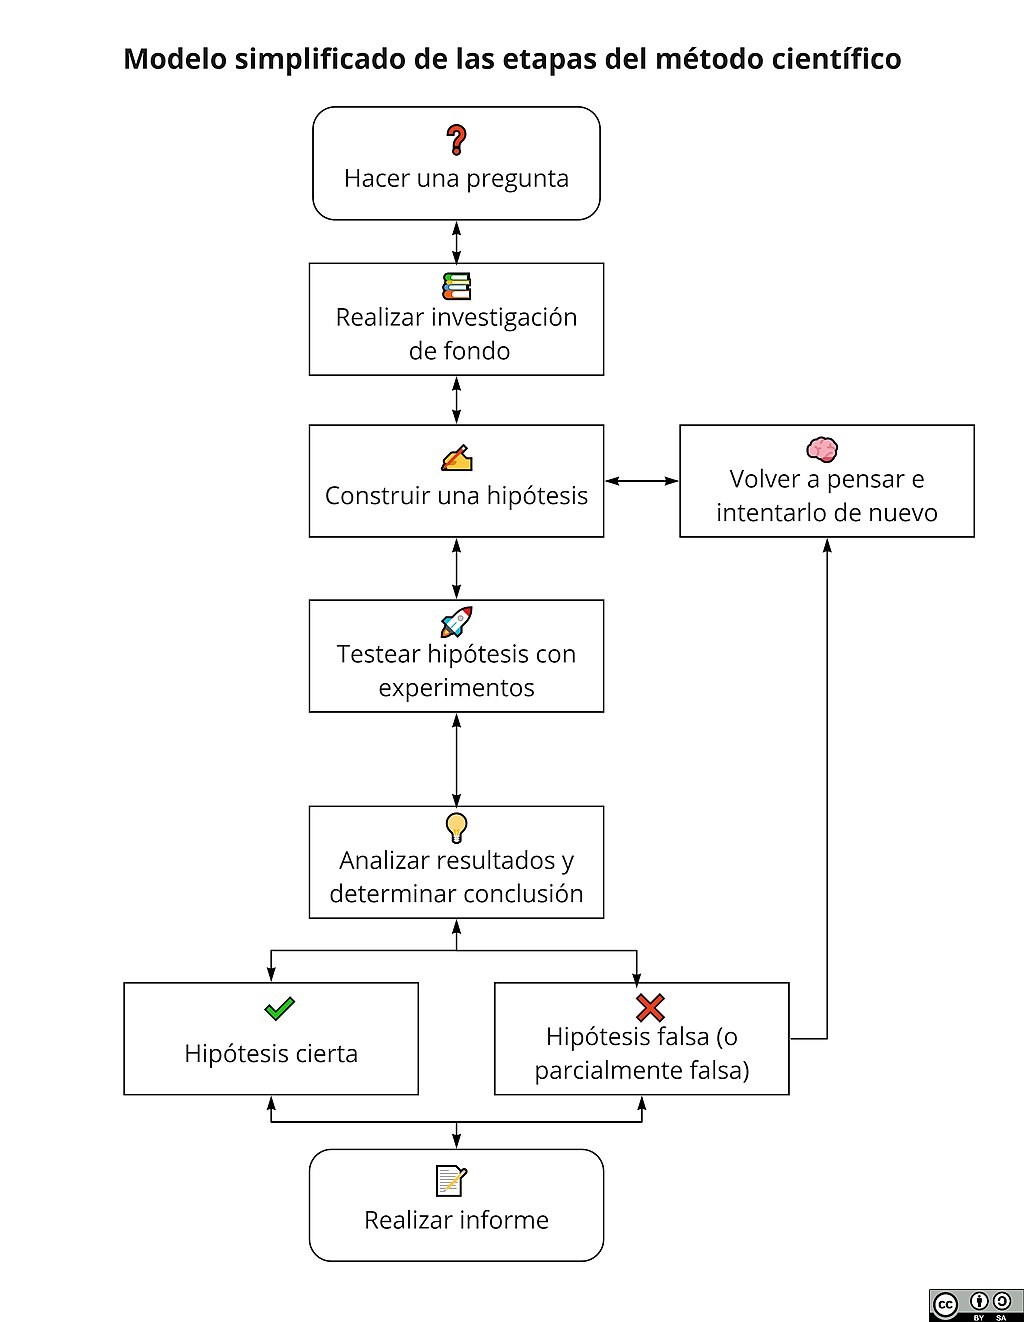
\includegraphics[width=.8\textwidth]{images/Método_científico_2021.jpg}
    \caption{Diagrama que representa el método científico.}\label{fg_met_cientifico}% \textcolor{red}{DEBE GENERARSE CON TIKZ. ESTO ES UN BORRADOR. Fuente: \url{https://es.wikipedia.org/wiki/M\%C3\%A9todo_cient\%C3\%ADfico\#/media/Archivo:M\%C3\%A9todo_cient\%C3\%ADfico_2021.jpg}}
\end{figure}

\begin{itemize}
    \item \textbf{Hacer una pregunta}. Todo trabajo científico comienza con la identificación de un problema, de una necesidad, de una carencia, en definitiva, de un ``¿a qué se debe esto?'' o ``¿cómo puedo resolver esto?'', o lo que anglosajones denominan \textit{gap}. Si no existe esta pregunta, problema o necesidad, deja de tener sentido el invertir tiempo y esfuerzo, y por ende dinero, en la realización de una experimentación cuyo fin no está asociado a ofrecer una respuesta útil.
    %\textbf{Hacer una pregunta}. Todo trabajo científico comienza con la identificación de un problema, de una necesidad, de una carencia, en definitiva, de un ¿a qué se debe esto? o ¿cómo puedo resolver esto?, o lo que anglosajones denominan \textit{gap}. Si no existe esta pregunta, problema o necesidad, deja de tener todo sentido el invertir tiempo y esfuerzo, y por ende dinero, en la realización de una experimentación cuyo fin no está asociado a ofrecer una respuesta útil.

    \item \textbf{Estudiar el estado del arte}. La identificación de una necesidad o el surgimiento de una pregunta científica no implica que ésta sea novedosa o que no tenga ya una respuesta. Por consiguiente, las acciones que intervienen en esta fase son: \begin{enumerate*}[label=(\arabic*)] \item identificar la disciplina científica donde se encuadra la pregunta a responder; \item analizar la novedad de la pregunta identificada, así como si ha sido ya respondida; y \item en caso de que el reto sí sea novedoso, estudiar la investigación relacionada con el ánimo de aprender los métodos ya usados, y emplearlos como inspiración en el diseño de la metodología o método original que de respuesta al desafío en estudio.\end{enumerate*}
    %\textbf{Estudiar el estado del arte}. La identificación de una necesidad o el alumbramiento de una pregunta científica, no implica que esta sea novedosa o que no tenga ya una respuesta. Por consiguiente, las acciones que intervienen en esta fase son: \begin{enumerate*}[label=(\arabic*)] \item identificar la disciplina científica donde se encuadra la pregunta a responder; \item analizar la novedad de la pregunta identificada, así como si ha sido ya respondida; y \item en caso de que el reto sí sea novedoso, estudiar la investigación relacionada con el ánimo de aprender los métodos ya usados, y emplearlos como inspiración en el diseño de la metodología o método original que de respuesta al desafío en estudio.\end{enumerate*}

    \item \textbf{Construir una hipótesis}. Una vez estudiado el estado del arte relacionado con el problema se debe definir una hipótesis sobre la cual se diseñará la solución y se evaluará si se confirma y, por tanto, resolverá el reto o si se desecha, y en consecuencia, se tendrá que definir otra hipótesis.
    %\textbf{Construir una hipótesis}. Una vez estudiado el estado del arte relacionado con el problema, se debe definir una hipótesis, sobre la cual se diseñará la solución y se evaluará si se confirma, y por tanto resolverá el reto, o si se desecha, y en consecuencia tener que definir otra hipótesis.

    \item \textbf{Evaluar la hipótesis}. Esta fase se compone de las siguientes acciones: \begin{enumerate*}[label=(\arabic*)]\item diseñar y desarrollar una metodología o método acorde a la hipótesis; \item diseñar un conjunto de experimentos que permitan evaluar la metodología o método desarrollado; y \item evaluar con métricas de evaluación estándares y propias del área en la que se circunscribe el problema de investigación con el fin de ofrecer una evaluación objetiva y comparable. Así mismo, se recomienda ofrecer todos los detalles de desarrollo y de evaluación con el ánimo de que la experimentación sea reproducible por cualquier investigador. Esta recomendación contribuye a confiar en la experimentación realizada, en el método o metodología propuesta, además de continuar la transferencia de conocimiento y el progreso científico.\end{enumerate*}
    %\textbf{Evaluar la hipótesis}. Esta fase se compone de las siguientes acciones: \begin{enumerate*}[label=(\arabic*)]\item diseñar y desarrollar una metodología o método acorde a la hipótesis; \item diseñar un conjunto de experimentos que permitan evaluar la metodología o método desarrollado; y \item evaluar con métricas de evaluación estándares y propias del área donde se circunscribe el problema de investigación con el fin de ofrecer una evaluación objetiva y comparable. Así mismo, se recomienda ofrecer todos los detalles de desarrollo y de evaluación, con el ánimo de que la experimentación sea reproducible por cualquier investigador. Este recomendación contribuye a confiar en la experimentación realizada, en el método o metodología propuesta, a la transferencia de conocimiento y al progreso científico.\end{enumerate*}

    \item \textbf{Analizar los resultados}. Esta fase es la más determinante, porque en función de su resultado, se podrá decir que se acepta la hipótesis, y por tanto se concluye que el método o metodología desarrollados resuelven el desafío objeto de estudio; o por el contrario se rechaza la hipótesis. Este rechazo implica que se debe volver a la definición de la hipótesis, o dicho de otro modo, a modificar la hipótesis y desarrollar otro método o metodología acorde a la nueva hipótesis.
    %\textbf{Analizar los resultados}. Esta fase es la más determinante, porque en función de su resultado, se podrá decir qu se acepta la hipótesis, y por tanto se concluye que el método o metodología desarrollados resuelven el desafío objeto de estudio, o por el contrario se rechaza la hipótesis. Este rechazo implica que se debe volver a la definición de la hipótesis,  o dicho de otro modo, a modificar la hipótesis y desarrollar otro método o metodología acorde a la nueva hipótesis.
\end{itemize}

Al igual que el método científico guía la labor de los investigadores de cualquier área, también debe ser la base de un TFG de investigación.

% ------------------------------------------------------------

%Definición de investigación.
%La investigación es un actividad intelectual y experimental realizada de modo sistemático con el propósito de aumentar los conocimientos sobre una determinada materia\footnote{Real Academia Española - \url{http://rae.es}}. En otras palabras, la investigación busca adquirir nuevos conocimientos y/o resolver problemas teóricos o prácticos mediante una actividad metódica y \underline {reproducible}. Para poder llevar a cabo una investigación exitosa es necesario tener en cuenta los siguientes elementos: 
%\begin{itemize}
%    \item Recopilar toda la información relevante sobre el problema a tratar utilizando fuentes heterogéneas y fiables.
%    \item Indagar sobre otros estudios ya realizados y publicados en la literatura científica sobre la misma problemática, analizando sus beneficios y sus limitaciones.
%    \item Seguir una metodología científica para poder así desarrollar el trabajo de manera organizada y coherente.
%    \item Mostrar los resultados obtenidos y valorarlos de forma objetiva sin omisiones.
%    \item Asegurar la reproducibilidad del trabajo, permitiendo que el tribunal o cualquier otra persona interesada sea capaz de verificarlo y replicarlo.
%\end{itemize}

%Conocimiento previo sobre el estado de la cuestión.
%Estructura del marco teórico y conceptual.
%De esta lista de elementos haremos especial hincapié en proveer de un marco teórico y conceptual que permita al tribunal, y a cualquier otro potencial lector, de la información básica necesaria para comprender la investigación realizada. De todas las tipologías de TFG de esta sección, la tipología de TFG de investigación es, probablemente, la que lleve más páginas dedicadas al estado del arte. Por tanto, también la bibliografía utilizada será más extensa. Debe de quedar claro que comprendes la temática y conoces qué cosas se han hecho ya y qué falta por hacer.

%Importancia de partir de una pregunta de partida.
%Otro punto importante a destacar en la memoria de los TFGs de investigación es la motivación del trabajo. No hay que confundir el apartado de motivación con una motivación personal. La motivación del trabajo, en este tipo de tipología de TFG, se refiere a identificar una brecha en el conocimiento actual del tema a tratar y de cómo la investigación en ese punto puede ayudar a contribuir en al área de estudio. Por tanto la motivación del trabajo debe incluirse en la memoria luego del estudio del estado del arte, ya que es muy posible que debas hacer referencia a algún punto ya tratado.

%Una vez detallado el problema de estudio y la motivación del TFG, es momento de hablar de los objetivos del trabajo. Para poder definir correctamente estos objetivos es necesario primero definir las hipótesis de partida, ya que la verificación o no de estas hipótesis serán justamente los objetivos principales del TFG. En el proceso de formulación de hipótesis debes plantear posibles respuestas a las preguntas surgidas durante tu análisis del estado del arte. Recuerda que las hipótesis deben poder ser verificables y falsables, es decir, susceptibles de ser refutadas.
   
En el siguiente apartado veremos en más detalle cómo debes llevar a cabo un TFG de investigación siguiendo una serie de pasos que te aseguren que los resultados obtenidos sean fiables y de calidad.

\subsection{Estructura del trabajo y de la memoria}
\label{tfx_inv_s_est_trabajo_memoria}

La estructura de la memoria no debe por qué distar mucho del resto de tipologías, pero sí debe recoger de forma adecuada el desarrollo científico realizado. Esto obliga a que el trabajo científico siga unas pautas coherentes que te dirijan, al menos, la labor experimental de una forma ordenada y dirigida a la evaluación con éxito de la hipótesis. El método científico, presentado en la sección \ref{tfx_inv_s_met_cientifico} es una guía muy recomendable para que orientes toda la actividad experimental y la redacción de la memoria. Por ende, la memoria debe reflejar: \begin{enumerate*}[label=(\arabic*)]\item la existencia de una necesidad de investigación, \item que esta no haya sido aún resuelta, o por lo menos no completamente, \item la definición de una hipótesis, \item el análisis, diseño e implementación del método o metodología que lleve a cabo la hipótesis y \item la evaluación de esta.\end{enumerate*} A continuación, se presentará una correspondencia entre el método científico y la estructura de la memoria, que a su vez ordena todo el trabajo relacionado con esta tipología de TFG.
%La estructura de la memoria no debe por qué distar mucho del resto de tipologías, pero sí debe recoger de forma adecuada el desarrollo científico realizado. Esto obliga a que el trabajo científico siga unas pautas coherentes que dirijan, al menos, la labor experimental de una forma ordenada y dirigida a la evaluación con éxito de la hipótesis. El método científico, presentado en la sección \ref{tfx_inv_s_met_cientifico}, es una guía muy recomendable para orientar todo la actividad experimental y la redacción de la memoria. Por ende, la memoria debe reflejar: \begin{enumerate*}[label=(\arabic*)]\item la existencia de una necesidad de investigación, \item que esta no haya sido aún resuelta, o por lo menos no completamente, \item la definición de una hipótesis, \item el análisis, diseño e implementación del método o metodología que lleve a cabo la hipótesis y \item la evaluación de esta.\end{enumerate*} A continuación, se presentará una correspondencia entre el método científico y la estructura de la memoria, que a su vez ordena todo el trabajo relacionado con esta tipología de TFG.

\paragraph{Motivación - Pregunta de investigación\textnormal{.}} En el primer capítulo o el capítulo de introducción del TFG debes recoger la motivación del trabajo, es decir, la razón por la cual lo realizas y merece la pena esforzarse en él durante los meses que involucre su realización. Esto que, en un inicio parece complicado: consiste en encontrar un reto que tenga asociada una pregunta científica, como podría ser: `\textit{¿es posible la generación de texto coherente y preciso para ofrecer información sobre trastornos de la conducta alimenticia?}''. Si has llegado a esa pregunta, es que existe una necesidad ligada a un problema, que a su vez tiene un contexto. Esta conjunción de contexto, problema, necesidad y pregunta científica es lo que debe constituir tu motivación del TFG, y la cual lo convierte en atractivo para cualquier lector, y sobre todo para la comunidad científica.
%\paragraph{Motivación - Pregunta de investigación} El primer capítulo o capítulo de introducción del TFG debe recoger la motivación del trabajo, es decir, la razón por la cual se realiza, merece la pena esforzarse en él durante los meses que involucre su realización, es interesante para cualquier lector, y representa un avance científico. Esto que parece complicado consiste en encontrar un reto que tenga asociado una pregunta científica, como podría ser \textit{¿es posible la generación de texto coherente y precisa para ofrecer información sobre trastornos de la conducta alimenticia?} Si se ha llegado a esa pregunta, es que existe una necesidad ligada a una problema, que a su vez tiene un contexto. Esta conjunción de contexto, problema, necesidad y pregunta científica es lo que constituye la motivación del TFG, y la cual lo convierte en atractivo para cualquier lector, y sobre todo para la comunidad científica.

\paragraph{Investigación relacionada - Estudiar el estado del arte\textnormal{.}} Una vez que ya se ha fijado el problema o pregunta a resolver, tienes que realizar las siguientes acciones:

\begin{enumerate}
    \item \textbf{Determinar el área de investigación}. La Ingeniería Informática abarca distintas áreas científicas, por lo que lo primero es saber si la pregunta se responde desde, por ejemplo, la informática teórica, la informática gráfica, la inteligencia artificial, la electrónica, o incluso si precisa de conocimiento externo a la Ingeniería Informática, como podría ser una investigación en un dominio interdisciplinar (medicina, biología, química, etc.). Atendiendo a la pregunta anterior, si te estás  cuestionando sobre la posibilidad de generar automáticamente lenguaje, parece que se trataría de un problema de inteligencia artificial, dado que se pide imitar un comportamiento característico de la inteligencia humana. En este ejemplo, una vez fijado que el área es la de la inteligencia artificial, el siguiente paso sería identificar la disciplina especializada en el desafío en cuestión, que en este ejemplo sería el procesamiento del lenguaje natural, ya que es la disciplina de inteligencia artificial encargada del desarrollo de métodos y metodologías computacionales orientados a la comprensión y generación de lenguaje por parte de un ordenador. Así mismo y siguiendo el ejemplo, necesitarías de cierto conocimiento externo, en particular sobre los trastornos alimenticios y cómo podría ayudar a su diagnóstico, prevención o tratamiento un sistema informático.
    %\textbf{Determinar el área de investigación}. La Ingeniería Informática abarca distintas áreas científicas, por lo que lo primero es saber si la pregunta se responde desde por ejemplo la informática teórica, la informática gráfica, la inteligencia artificial, la electrónica, o incluso si precisa de conocimiento externo a la Ingeniería Informática, como podría ser una investigación en el dominio de la biología. Atendiendo a le pregunta anterior, si se está cuestionando sobre la posibilidad de generar automáticamente lenguaje, parece que se trataría de un problema de inteligencia artificial, dado que se pide imitar un comportamiento característico de la inteligencia humana como es la generación de lenguaje. Una vez fijada que el área es la de la inteligencia artificial, el siguiente paso sería identificar la disciplina especializada en el desafío en cuestión, que en este caso sería el procesamiento del lenguaje natural, ya que es la disciplina de inteligencia artificial encargada del desarrollo de métodos y metodologías computacionales orientados a la comprensión y generación de lenguaje por parte de un ordenador.

    \item \textbf{Búsqueda de los trabajos más relevantes}. Conocida el área y disciplina de investigación, es momento de buscar los trabajos relacionados con la pregunta de investigación. En el caso particular que estamos tratando, serían modelos de generación de lenguaje. Con este dato, ya es momento de que estudies todo lo relacionado con la problemática, y seleccionar los avances más recientes. En este caso se corresponderían con los grandes modelos de lenguaje, y sus diversas formas de aplicación para generar lenguaje que dé respuesta a distintas situaciones en función del caso de uso. En el ejemplo que estamos siguiendo se podría pensar que una posible aplicación de los grandes modelos de lenguaje podría ser aplicarlos en modo de sistemas de recuperación de información.
    %\textbf{Búsqueda de los trabajos más relevantes}. Conocida el área y disciplina de investigación, es momento de encontrar los trabajos relacionados con la pregunta de investigación. En el caso particular que estamos tratando, serían modelos de generación de lenguaje. Con este dato, ya es momento de estudiar todo lo relacionado con la problemática, y seleccionar los avances más recientes. En este caso se corresponderían con los grandes modelos de lenguaje.

    \item \textbf{Evaluación de si el reto está resuelto\textnormal{.}} Tras la selección de los trabajos más importantes, tienes que evaluar si el desafío planteado está o no resuelto. En caso de que así sea, deberás plantear uno nuevo hasta que encuentres aquel que aún no lo esté. Por contra, si no lo está, la pregunta representa un verdadero reto sobre el que merece la pena realizar el TFG.
    %\textbf{Evaluación de si el reto está resuelto}. Tras la selección de los artículos más importantes es momento de evaluar si el desafío planteado está resuelto. En caso de que así sea, se deberá revaluar la pregunta de investigación, hasta encontrar aquella que aún no lo esté. Por contra, si no lo está, la pregunta representa un verdadero reto sobre el que merece la pena trabajar.
    
    Pudiera parecer que el trabajo de esta fase termina aquí, pero no es así, porque ahora es el momento en el que determinarás las estrategias seguidas hasta la fecha, con el fin de realizar una propuesta novedosa que pueda compararse con lo existente, y que ofrezca mejores resultados.
    %Pudiera parecer que el trabajo de esta fase termina aquí, pero no es así, porque ahora es momento de determinar las estrategias seguidas hasta la fecha con el fin de realizar una propuesta novedosa que pueda compararse con lo existente, y que ofrezca unos mejores resultados.
\end{enumerate}

El resultado de este estudio sobre trabajos relevantes y sus estrategias lo reflejarás en un capítulo específico sobre el estado de la investigación asociada al proyecto. Algunos ejemplos de nombres que puede tener este capítulo son: contexto, estado de arte, estado de la cuestión, trabajos relacionados, o el nombre específico de la disciplina de investigación asociada al desafío científico del TFG.
%El resultado de este estudio deberá reflejarse en un capítulo específico sobre el estado de la investigación asociada al proyecto. Algunos ejemplos de nombres que puede tener este capítulo son: contexto, estado de arte, estado de la cuestión, trabajos relacionados o el nombre específico de la disciplina de investigación asociada al desafío científico del TFG.

\paragraph{Hipótesis\textnormal{.}} Un conocimiento profundo del problema científico asociado te prepara para la enunciación de la hipótesis del TFG. Esta es una suposición de estrategia, metodología o modelo a desarrollar para resolver el desafío científico en el que estás trabajando. Así mismo, si la evaluación de la hipótesis la confirma, conlleva haber propuesto una solución válida al reto científico del TFG. Automáticamente se podría pensar que un resultado negativo implica el fracaso del trabajo científico desarrollado. Esto no tiene por qué ser así, dado que de los resultados negativos también se pueden obtener conclusiones positivas, que incluso pueden servir de base para posteriores avances científicos. Por tanto, no te agobies si no obtienes los buenos resultados que esperabas. 

Siguiendo el ejemplo que está guiando la descripción de la estructura del trabajo y memoria, una posible hipótesis sería: las arquitecturas basadas en recuperación de información aumentada (\textit{retrieval augmented generation}, RAG) pueden generar texto coherente para ayudar a personas con trastornos de la conducta alimentaria. Esta hipótesis conllevaría al diseño, implementación y evaluación científica y de software de un sistema tipo RAG para el caso de uso indicado.
%\paragraph{Hipótesis} Un conocimiento profundo del problema científico asociado prepara para la enunciación de la hipótesis del TFG. Esta es una suposición de estrategia, metodología o modelo a desarrollar para resolver el desafío científico en el que se está trabajando. Así mismo, si la evaluación de la hipótesis la confirma, conlleva haber propuesto una solución válida al reto científico del TFG. Automáticamente se podría pensar que un resultado negativo implica el fracaso del trabajo científico desarrollado. Esto no tiene por qué ser así, dado que de los resultados negativos también se pueden obtener conclusiones muy positivas, que incluso pueden servir de base para posteriores avances científicos.

Se recomienda que también indiques la hipótesis en el capítulo de introducción, ya que va asociada a la pregunta de investigación. Así mismo, una vez formulada la hipótesis, ya se puedes establecer los objetivos e hitos del TFG, los cuales son una forma de concretar el trabajo a realizar.
%La hipótesis se recomienda que también se indique en el capítulo de introducción, porque va asociada a la pregunta de investigación. Así mismo, una vez formulada la hipótesis, ya se puede establecer los objetivos e hitos del TFG, los cuales son una forma de concretizar el trabajo a realizar.

\paragraph{Desarrollo - Evaluación de la hipótesis\textnormal{.}} Para poder probar la validez de tu hipótesis, antes tienes que desarrollar la metodología o método subyacente a la misma. Por tanto, hay que diseñar primeramente el marco experimental. En la mayoría de los casos el marco experimental va a seguir los cánones de la investigación cuantitativa, la cual requiere de una evaluación empírica. Esto obliga a seleccionar el conjunto o conjuntos de datos sobre los que vas a realizar la evaluación, y a determinar las medidas de evaluación a emplear.
%\paragraph{Desarrollo - Evaluación de la hipótesis} Para poder probar la validez de la hipótesis, antes hay que desarrollar la metodología o método subyacente a la misma. Por tanto, se debe comenzar primeramente con el diseño del marco experimental. En la mayoría de los casos, el marco experimental va a seguir los cánones de la investigación cuantitativa, la cual requiere de una evaluación empírica. Esto obliga a seleccionar el conjunto o conjuntos de datos sobre los que realizar la evaluación, y a determinar las medidas de evaluación a usar.

La elección del conjunto de datos es una decisión muy importante del proceso de evaluación, porque si estos no son de calidad, o no son representativos, la calidad y credibilidad del marco experimental se verá resentido. En cualquier caso, siempre tienes que describir los datos elegidos, y en caso de que no sean propios, haz referencia a su fuente. A continuación te mostramos algunos ejemplos de conjuntos de datos que se pueden usar:
%La elección del conjunto de datos es una decisión muy importante del proceso de evaluación, porque si estos no son de calidad o no son representativos, la calidad y credibilidad del marco experimental se verá resentido. En cualquier caso, siempre hay que describir los datos elegidos, y en caso de que no sean propios hacer referencia a su fuente. A continuación algunos ejemplos de conjuntos de datos que se pueden usar:

\begin{itemize}
    \item {\bf Conjuntos de datos externos}: Si trabajas con conjuntos de datos públicos y ampliamente conocidos por la comunidad científica es sencillo hacer referencia a ellos en la memoria. Se recomienda utilizar una tabla para mostrar comparativamente los distintos conjuntos de datos empleados, como en el ejemplo de la tabla \ref{tab:uci}. Puedes incorporar a la tabla las columnas que sean necesarios y que incluyan toda la información sobre la cual haces referencia en el texto principal de la memoria. Presta atención al texto que acompaña a la tabla en donde se indica tanto el origen de los datos como una cita o referencia online a ellos. 

\begin{table}[!ht]
\centering
\caption[Conjuntos de datos utilizados en este trabajo provenientes del repositorio UCI]{Conjuntos de datos utilizados en este trabajo provenientes del repositorio UCI\footnotemark.\label{tab:uci}}
\begin{tabular}{cccccc}
\hline
 & \textbf{No. de} & \textbf{No. de} & \multicolumn{3}{c}{\textbf{No. de Atributos}} \\
{\it \textbf{Dataset}} & \textbf{Casos} & \textbf{Clases} & \textbf{Nominales} & \textbf{Numéricos} & \textbf{Perdidos}\\ \hline
Anneal & 898 & 6 & 32 & 6 & 29 \\
Breast Cancer & 286 & 2 & 9 & 0 & 2 \\
Diabetes & 768 & 2 & 8 & 0 & 8 \\
Heart-C & 303 & 5 & 7 & 6 & 2 \\
Hepatitis & 155 & 2 & 13 & 6 & 15 \\
House Votes & 435 & 2 & 16 & 0 & 16 \\
Iris & 150 & 3 & 0 & 4 & 0 \\
Lymphography & 148 & 4 & 15 & 3 & 0 \\
Vowel & 990 & 11 & 3 & 10 & 0 \\
Wine & 178 & 3 & 0 & 13 & 0 \\
Zoo & 101 & 7 & 16 & 1 & 0 \\
\hline
\end{tabular}
\end{table}
\footnotetext{\url{https://archive.ics.uci.edu/}}

    \item {\bf Conjuntos de datos propios}: si dentro de tu propuesta de trabajo incluyes la generación de conjuntos de datos propios, recogidos a partir de un experimento real o cuestionarios pasados a usuarios, por ejemplo, entonces necesitas crear un apartado en la memoria para detallar todo el proceso. Si por otro lado, el conjunto de datos te lo ha dado tu tutor, entonces necesitas detallar su origen y características. Si es posible, incluye el o los conjuntos de datos al entregar la memoria. Si por alguna razón los datos son privados o no tienes permiso para difundirlos debes entonces explicarlo detalladamente. Recuerda que para trabajar con datos con información de carácter personal, antes debes anonimizarlos. 
    \item {\bf Conjuntos de datos artificiales}: si cuentas con conjuntos de datos creados artificialmente, también llamados datos sintéticos, debes explicar cómo se han generado. Si el procedimiento de generación de estos datos es propuesta tuya, entonces descríbelo con detalle como se explica en el apartado anterior. En caso de ser generados por terceras partes entonces basta con referenciar ese trabajo y explicar brevemente cómo se realiza este proceso. Igualmente para ambos casos necesitas mostrar en una tabla una descripción de los conjuntos de datos, como puedes ver en la tabla \ref{tab:fake}. Recuerda que tu trabajo debe de poder ser reproducible por cualquier persona, por tanto debes incluir en el material a entregar los conjuntos de datos que hayas generado tú o un enlace a aquellos generados por terceras personas.

\begin{table}[!ht]
\centering
\caption{Elementos incluidos en los distintos conjuntos de datos generados artificialmente.}
\label{tab:results}
\begin{tabular}{c|ccc}
\hline
{\it \textbf{Dataset}} & \textbf{Edificio} & \textbf{Árbol} & \textbf{Persona} \\
\hline
Sintético A & 5 & 10 & 4 \\
Sintético B & 0 & 12 & 11 \\
Sintético C & 1 & 2 & 2 \\
Sintético D & 3 & 2 & 3 \\
Sintético E & 4 & 5 & 1 \\
\hline
\end{tabular}
\label{tab:fake}
\end{table}
\end{itemize}

El siguiente paso es \textbf{diseñar e implementar la metodología o modelo}. Se podría decir que esta parte del TFG es para la que estás más preparado/a, por ser la de mayor contenido técnico. El diseño y desarrollo deben seguir los principios de ingeniería aprendidos durante la carrera, siendo recomendable que tú tomes decisiones propias en el ámbito de elección de lenguaje de programación, de bibliotecas a usar y de entorno de programación a utilizar.
%El siguiente paso es \textbf{diseñar e implementar la metodología o modelo}. Se podría decir que esta parte del TFG es para la que está más preparado el alumno, por ser la de mayor contenido técnico. El diseño y desarrollo deben seguir los principios de ingeniería aprendidos durante la carrera, siendo recomendable que el alumno tome decisiones en el ámbito de elección de lenguaje de programación, de librerías a usar y de entorno de programación a utilizar.

Antes de proseguir, nos gustaría hacerte la recomendación de que este tipo de TFG estuvieran acompañados de un demostrador, es decir, de integrar la propuesta científica en un sistema informático que muestre su utilidad. Si se opta por ello, el desarrollo del demostrador debe seguir las recomendaciones de la ingeniería del software, lo que implica: \begin{enumerate*}[label=(\arabic*)]\item elección de metodología de trabajo, \item realización de fase de análisis, \item diseñar la solución, \item implementar el diseño y \item validar y evaluar el software desarrollado.\end{enumerate*} Es muy recomendable la realización de un demostrador, porque te permite mostrar los conocimientos adquiridos durante la carrera, sobre todo los relativos a los procesos y principios de la ingeniería del software. Siguiendo con el ejemplo, si ha implementado un sistema informático basado en una arquitectura RAG para facilitar el acceso a la información sobre trastornos de la conducta alimenticia, un posible demostrador sería un \textit{chat} conversacional, de forma que el usuario experimente la consulta de información como si estuviera conversando en otro tipo de \textit{chat} a los que suele estar acostumbrado en \textit{Whatsapp} o \textit{Telegram}.
%Ante de proseguir, quisiera hacerse la recomendación de que este tipo de TFG estuvieran acompañados de un demostrador, es decir, de integrar la propuesta científica en un sistema informático que muestre su utilidad. Si se opta por ello, el desarrollo del demostrador debe seguir las recomendaciones de la ingeniería del software, lo que implica: \begin{enumerate*}[label=(\arabic*)]\item elección de metodología de trabajo, \item realización de fase de análisis, \item diseñar la solución, \item implementar el diseño y \item validar y evaluar el software desarrollado.\end{enumerate*} Es muy recomendable la realización de un demostrador, porque permite que el alumno muestre los conocimientos adquiridos durante la carrera, sobre todo los relativos a los procesos y principios de la ingeniería del software.

Una vez concluida la implementación de la metodología o modelo pasamos a la fase de evaluación. Ésta debe realizarse con las medidas de evaluación usadas en los trabajos de investigación relacionados. Esto es relevante porque permite comparar la propuesta del TFG con la literatura, y así poder saber si la propuesta representa realmente un avance o no. Además, se recomienda facilitar la comparación con el estado del arte por medio de una tabla comparativa con los modelos más relevantes. No olvidar que para poder decir, por ejemplo, que un algoritmo es mejor que otro, es necesario no solo realizar múltiples experimentos, sino también someter los resultados obtenidos a análisis estadísticos. Recuerda que los experimentos que realizas deben poder reproducirse, por tanto no olvides fijar una semilla para que, por ejemplo, en caso de usar un generador de números aleatorios, tu trabajo sea reproducible. 

Atendiendo a nuestro ejemplo, la evaluación tendría que realizarse con métodos y librerías o \textit{frameworks} propios de la comunidad para evaluar sistemas basados en RAG. Actualmente el \textit{framework} de evaluación más extendido es RAGAS\footnote{\url{https://docs.ragas.io/en/latest/}} \cite{esetal2024Ragas}, el cual integra medidas clásicas de recuperación de información (precisión y cobertura (\textit{recall})) y métricas para valorar la calidad del texto generado. En cuanto a la reproducibilidad, tendrás que indicar todos los detalles de la representación semántica usada\footnote{Se correspondería a modelos de \textit{word embeddings} contextualizados, y en la mayoría de los casos basados en \textit{sentence transformers.}}, compartir si es posible dicha representación, el número de contextos usados, publicar la acción a modo de consulta\footnote{Conocido en la comunidad científica y profesional como \textit{prompt}.} para que el modelo de lenguaje genere la respuesta, así como todos los parámetros de configuración de este. En el caso de que sean particulares y exclusivos del TFG, te recomendamos que lo pongas a disposición de la comunidad. Esto que se indica para el caso particular del ejemplo debes adaptarlo a tu TFG particular y al área de investigación que se circunscriba tu trabajo.
%Una vez concluida la implementación de la metodología o modelo se debe evaluar. La evaluación debe realizarse con las medidas de evaluación usadas en los trabajos de investigación relacionados. Esto es relevante porque permite comparar la propuesta del TFG con la literatura, y así poder saber si la propuesta representa realmente un avance o no. Además, se recomienda facilitar la comparación con el estado del arte por medio de una tabla comparativa con los modelos más relevantes.

En cuanto a la organización de la evaluación de la hipótesis en varias secciones o capítulos, dependerá de su extensión y de si se realiza un sistema demostrador. En el caso de que se haga un sistema informático, se recomienda separar en capítulos las distintas fases del proceso de desarrollo de software. En caso contrario, puede que solo sea necesario elaborar un capítulo describiendo todo lo relativo a la elección de datos, implementación y evaluación.
%En cuanto a la organización de la evaluación de la hipótesis en capítulos, todo va a depender de su extensión y de si se realiza un sistema demostrador. En el caso de que se haga un sistema informático, se recomienda separar en capítulos las distintas fases del proceso de desarrollo de software. En caso contrario, puede que solo sea necesario elaborar un capítulo describiendo todo lo relativo a la elección de datos, implementación y evaluación.

\paragraph{Análisis de los resultados\textnormal{.}} El análisis de los resultados y la comparación con el estado del arte es el momento decisivo en esta tipología de TFG, debido a que determina si la hipótesis se acepta o no. En el caso de que se acepte, el trabajo no concluye aquí, ya que se recomienda realizar un análisis tanto de los aciertos, como de los errores que se hayan producido. Estos permitirán realmente entender cómo el modelo o metodología desarrollados están dando respuesta al reto de investigación.
%\paragraph{Análisis de los resultados} El análisis de los resultados y la comparación con el estado del arte es el momento decisivo de esta tipología de TFG, debido que determina si la hipótesis se acepta o no. En el caso de que se acepte, el trabajo no concluye aquí, ya que se recomienda realizar un análisis tanto de los aciertos, como de los errores que se hayan producido, dado que estos permitirán realmente entender cómo el modelo o metodología desarrollados están dando respuesta al reto de investigación.

En caso de que la hipótesis sea rechazada, se debe evaluar si un análisis profundo de los resultados puede ser interesante para la comunidad científica, y por tanto constituir una contribución importante para el TFG. Este análisis puede concluir que se deben elegir otros datos, que el reto ha llegado a un escenario de resultados tope, que la estrategia algorítmica no es la adecuada y que se deben seguir otras, o que la elección de las características y los parámetros de configuración del algoritmo no han sido los óptimos. Esto que pudiera parecer una fracaso, puede ser la base de futuros progresos porque ofrece a la comunidad científica un conjunto de lecciones aprendidas a tener en cuenta para posteriores desarrollos. Ahora bien, se remarca que cuando se ha obtenido un resultado negativo, el análisis de resultados debe ser profundo y con conclusiones interesantes para considerarlo como una contribución y como un TFG válido.
%En caso de que la hipótesis sea rechazada, se debe evaluar si un análisis profundo de los resultados puede ser interesante para la comunidad investigadora, y por tanto constituir una contribución importante para el TFG. Este análisis puede concluir que se deben elegir otros datos, que el reto ha llegado a un escenario de resultados tope, que la estrategia algorítmica no es la adecuada y que se deben seguir otras o que la elección de las características y los parámetros de configuración del algoritmo no han sido los óptimos. Esto que pudiera parecer una fracaso, puede ser la base de futuros progresos porque ofrece a la comunidad científica un conjunto de lecciones a tener en cuenta para posteriores desarrollos. Ahora bien, se remarca que cuando se ha obtenido un resultado negativo, el análisis de resultados debe ser profuso y con conclusiones interesantes para considerarlo como una contribución y como TFG válido.

También es posible que los experimentos realizados tengan ciertas limitaciones que afecten a la interpretación de los resultados obtenidos. Debes, por tanto, abordar este tema de manera transparente. Las limitaciones son características del diseño o metodología que influyen en la validez, aplicabilidad o generalización de los hallazgos. Pueden derivarse del diseño inicial del estudio, del método utilizado o de desafíos imprevistos durante el proyecto. Existen distintos tipos de limitaciones, como las relacionadas con el diseño o la metodología del estudio, o bien de los datos en sí, que pueden presentar problemas de calidad, disponibilidad o fiabilidad. Reconocer estas limitaciones te brinda la oportunidad para proponer formas de abordar estas limitaciones y demuestra un pensamiento crítico.

\paragraph{Conclusiones.} El último capítulo debe ser el de conclusiones, que no debe ser una mera recapitulación del TFG, sino un lugar donde destacar si la propuesta permite aceptar la hipótesis, y los principales resultados del análisis a modo de lecciones aprendidas. En resumen, unas conclusiones que aporten valor al TFG. Adicionalmente puede ser útil añadir una lista de trabajos futuros en la que puedas demostrar que has comprendido el problema sobre el que has trabajado y propongas líneas de trabajo futuras a partir de tus conclusiones.
%\paragraph{Conclusiones} El último capítulo debe ser el de conclusiones, que no debe ser una mera recapitulación del TFG, sino un lugar donde destacar si la propuesta permite aceptar la hipótesis, y los principales resultados del análisis a modo de lecciones aprendidas. En resumen, unas conclusiones que aporten valor al TFG.


%Muchos de los algoritmos que se utilizan para minería de datos tienen una componente aleatoria. Esto quiere decir que dependiendo de la semilla del generador de números aleatorios utilizado puede darnos una respuesta diferente. Para evitar tener este sesgo es necesario ejecutar varias veces el mismo algoritmo utilizando distintas semillas. Normalmente se suele ejecutar unas 5 o 10 veces y luego tomar para cada métrica a medir su media y desviación estándar. De esta manera puedes deducir si el algoritmo es robusto, si tiene mucha variabilidad, etc. Por tanto, a la hora de reportar los resultados debes incluir tanto la media como la desviación estándar en la tabla de resultados, como puedes ver en la Tabla \ref{tab:sd}.

%\begin{table}[htbp]
%\centering
%\label{tab:cityscapes}
%\begin{tabular}{c|c|c|c}
%\hline
%\textbf{Método} & \textbf{Iris} & \textbf{Diabetes} & \textbf{Ionosphere} \\ 
%\hline
%K-means & 214 (289) & 2628 (175) & 805 (202) \\
%LKM & 169 (10) & 1691 (47) & 908 (34) \\ 
%DE-LKM &  1938 (151) & 7425 (214) & 9449 (55) \\
%LC-LKM & 3764 (2431) & 12797 (44) & 17653 (2298) \\
%EM & 255 (139) & 3033 (226) & 1688 (1301) \\
%\hline
%\end{tabular}
%\caption{Tiempo de ejecución en ms. (media y desviación estándar entre paréntesis) de las 10 ejecuciones de cada %algoritmo por conjunto de datos.\label{tab:sd}}
%\end{table}

%También es necesario realizar un proceso de entrenamiento o {\it training} y uno de prueba o {\it test} posterior. Para ello se puede dividir el conjunto de datos en una parte para training y otra para test. Sin embargo, la opción más recomendada es utilizar algún tipo de validación cruzada que divide el conjunto de datos original en varias partes. Luego se utilizan todas menos una para entrenar y la restante para validar. Esto se realiza tantas veces como divisiones del conjunto de datos original hemos hecho. Finalmente se reporta la media y la desviación estándar de las métricas evaluadas. En caso de utilizar particiones ya realizadas por terceros indícalo e incluye una referencia en la memoria y/o los ficheros mismos al entregarla.

\subsection{Recomendaciones}\label{tfx_inves_ss_recomendaiones}
%Sugerencias para futuros investigadores.
%Áreas de mejora o posibles extensiones del estudio.

A modo de buenas prácticas para la realización de este tipo de TFG, se proponen a continuación una serie de consejos que esperamos que sean de utilidad:
%A modo de buenas prácticas para la realización de este tipo de TFG, se proponen una seria de consejos que se estiman que allanarán su elaboración.

\begin{itemize}
    \item \textbf{Sistema demostrador}. Como ya se ha indicado, se recomienda realizar un sistema informático que integre la propuesta científica, con el fin de que puedas aplicar los principios de ingeniería de software adquiridos durante la carrera. 
    
    \item \textbf{Manual de instalación y uso}. En caso de no realizar un sistema demostrador, es esencial proveer de toda la información necesaria para asegurar la reproducibilidad de los resultados. Eso incluye un manual de instalación y uso, el código fuente utilizado, etc.

    \item \textbf{Experimentación y redacción en paralelo}. Es práctica común de los estudiantes el realizar primero la experimentación y posteriormente la redacción de la memoria. Esto suele conllevar agobio y hastío, dado que suele apetecer más el programar un sistema informático que redactar una memoria. Por tanto, para facilitar el proceso de redacción, y también para que este sea más rico, se recomienda realizar la tarea de experimentación y redacción en paralelo.

    \item \textbf{Registrar todo paso de la experimentación}. Es importante registrar todo paso del proceso científico que se realice, dado que facilitará luego su desarrollo en la memoria. Esto incluye el uso de sistemas de control de versiones, llevar un \textit{log} en el cual se detallen los distintos experimentos realizados, etc.

    \item \textbf{Continua interacción con la persona que te tutoriza}. Teniendo en cuenta que la metodología de investigación te puede resultar novedosa, es muy importante que tengas reuniones frecuentes con tu tutor o tutora,  con objeto de que te vayan guiando paso a paso, y en las que tendrás que aprovechar para consultar todas las dudas que te vayan surgiendo.

    \item \textbf{Trabajos futuros}. La investigación es un proceso continuo en el que cada investigador aporta su pequeño grano de arena. A medida que uno se sumerge dentro del área de estudio, van surgiendo nuevas ideas e hipótesis que por la extensión y cantidad de horas para realizar el TFG no pueden ser acometidas. Es importante por tanto dejarlas por escrito, en el apartado de conclusiones o uno propio, de forma que cualquier lector pueda retomar el trabajo realizado y extenderlo desde el punto en el que ha acabado el TFG.

    \item \textbf{Reproducibilidad}. Es muy importante que describas tu investigación con tal detalle que cualquier otra persona pueda reproducir de manera fehaciente todo el proceso que has realizado y obtener los mismos resultados. De esta forma podrá comparar sus propios resultados con los tuyos. Por desgracia, aunque es verdad que cada vez menos, te encontrarás con situaciones en las que te interesaría evaluar un modelo que ya ha sido publicado pero no tienes suficientes detalles para implementarlo tú, o no aportan información de valores de parámetros con los que han obtenido los resultados que se han publicado. Estas situaciones son bastante frustrantes pues, aunque el modelo sea interesante, similar al tuyo, utilice el mismo enfoque, o cualquier otra causa, no podrás emplearlo para comparar resultados. Por tanto, describe tus modelos y entornos experimentales con todo detalle. Incluso provee el código y los conjuntos de datos (siempre que puedas).

    \item \textbf{Un mal resultado también es un resultado}. La investigación puede llegar a ser a veces un proceso ingrato pues no se suelen obtener normalmente los resultados magníficos que uno espera. Muchas veces repetimos el ciclo de la figura \ref{fg_met_cientifico} varias veces y los resultados obtenidos no son los que deseamos. ¿Esto implica que debemos continuar \textit{sine die} con nuestro trabajo hasta conseguir buenos resultados? ¿Y si no los conseguimos significa que debemos abandonar el problema entre manos y cambiar de temática de TFG? La respuesta en ambas cuestiones es la misma y muy contundente: no. Si no conseguimos en un plazo razonable resultados que consideremos que realizan una contribución científica, tenemos que tener en cuenta que científicamente mostrar el camino por donde no se lleva a nada positivo es también una aportación, que será útil para otros investigadores (``por aquí, aunque parecía prometedor no podemos ir porque no conduce a nada''). Y para ti, pues desde el punto de vista de tu TFG estarás mostrando que eres capaz de realizar una investigación científica completa y eso en sí es suficiente para tu TFG. Ya tendrás tiempo en tu TFM o en tu tesis doctoral de continuar y encontrar alternativas que mejoren el estado del arte del problema entre manos.

    \item \textbf{Publica los resultados}. Una vez que tengas hecho todo el trabajo científico, ¿por qué no publicar los resultados en un congreso o en una revista y hacer partícipe a la comunidad científica nacional o internacional de la investigación que has realizado y de las conclusiones obtenidas? De esta forma publicitarás tu trabajo y otros investigadores podrán apoyarse en él para seguir avanzando. Además, que tu TFG esté avalado por una publicación científica siempre será una magnífica carta de presentación para la evaluación de tu TFG, sin contar con el hecho de que estarás empezando ha hacerte un currículum muy útil para una posterior fase profesional ya sea en la empresa o en la Universidad.
\end{itemize}


\section{TFG de revisión del estado del arte}
\label{appendix:revisionestado}

Existe una modalidad de TFG que es en sí una revisión del estado del arte. Para que nos entendamos es como la sección de revisión del estado del arte vista en el capítulo \ref{cap:RevisionEstadoDelArte} pero a lo grande, donde la revisión ocupa toda la memoria del TFG.

Si vas a realizar este tipo de TFG, en primer lugar te recomendamos que leas ese capítulo con objeto de obtener una idea general de qué es una revisión del estado del arte y, por supuesto, el capítulo \ref{cap:bibliografia} con el objetivo de tener claro cómo gestionar la bibliografía del TFG, pues, si ya es importante este asunto, en este tipo de proyecto fin de carrera, las referencias bibliográficas se configuran como algo vital.

El objetivo de esta sección será explicar brevemente cómo llevar a cabo la elaboración de la memoria de un trabajo de revisión del estado del arte. En este caso, hay mucho material publicado que puede serte de utilidad, por lo que haremos una revisión poco somera del mismo con objeto de ofrecerte algún material de inicio para que, al menos, comiences la tarea. Y de cualquier forma, ponte de acuerdo con la persona que te tutoriza sobre la forma de enfocar el trabajo, pues es un tipo muy especial de TFG que necesita ser definido y desarrollado de forma muy precisa.

\subsection{Tipos de revisiones}

Lluis Codina en \cite{codina2024lluis} establece dos grandes grupos de tipos de revisiones: las tradicionales o narrativas y las de tipo sistemático. Las primeras son más bien ensayos y carecen de validez científica; las segundas, sí que tienen esta validez, y se clasifican en sistemáticas, que se emplean para determinar el impacto de intervenciones, y de alcance, usadas para describir hasta dónde (alcance) llega un conocimiento dado. En este trabajo, el autor explica claramente cuándo se debería elegir un tipo u otro de revisión.

Pero esta es una simplificación que el profesor Codina ha realizado porque en realidad existe una gran cantidad de tipos diferentes de revisiones tal y como Grant y Booth indican en \cite{grant2009maria}, la mayoría ampliamente usados en el campo de las ciencias de la salud y con un componente estadístico muy fuerte:

\begin{itemize}
    \item Revisiones tradicionales. 
    \item Síntesis de conocimiento: de forma genérica se podrían definir como aquellas revisiones que contextualizan e integran los hallazgos de investigación de estudios individuales dentro del cuerpo más amplio de conocimiento sobre el tema que tengas entre manos. Algunos de los más conocidos y usados pueden ser los siguientes:
    \begin{itemize}
        \item Revisiones sistemáticas: identifican, evalúan y sintetizan todas las pruebas empíricas que cumplen unos criterios de elegibilidad previamente especificados. Las revisiones sistemáticas deben ser lo más exhaustivas e imparciales posibles.
        
        \item Metanálisis: subconjunto de revisiones sistemáticas que combina estadísticamente los resultados de estudios cuantitativos encontrados con objeto de ofrecer un efecto más preciso de los resultados.
        
        \item Revisiones de alcance: abordan una pregunta de investigación exploratoria destinada a extraer conceptos clave, tipos de evidencia y nichos en la investigación relacionada con un área o campo definido mediante la búsqueda sistemática, selección y síntesis del conocimiento existente.
        
        \item Revisiones rápidas: un tipo de síntesis de conocimiento en el cual los procesos de revisión sistemática se aceleran y los métodos se simplifican para completar la revisión más rápidamente que en el caso de las revisiones sistemáticas típicas, que vienen a tener un tiempo de realización de un año, reduciendo el tiempo de confección de cinco a doce semanas. Se emplean cuando no se dispone mucho tiempo para realizarlas.
        
        \item Revisiones realistas: comprenden y desentrañan los mecanismos por la que una intervención funciona (o no funciona), proporcionando así una explicación, en lugar de un juicio sobre cómo funciona.

        \item Revisiones mixtas: combinación de los hallazgos de estudios cualitativos y cuantitativos dentro de una sola revisión sistemática para abordar las mismas preguntas de revisión superpuestas o complementarias.
        
        \item Revisiones cualitativas: aquellas que integran o comparan los hallazgos de estudios cualitativos.
        
        \item Síntesis narrativas: se basa en el uso de palabras y texto para resumir y explicar los hallazgos de la síntesis más que en resultados estadísticos. Básicamente usan la palabra para ``contar la historia'' de los hallazgos de los estudios incluidos.

        \item Revisiones tipo paraguas: se refiere a una revisión que recopila evidencia de múltiples revisiones en un documento accesible y utilizable. 
        
    \end{itemize}
\end{itemize}

En este enlace \url{https://unimelb.libguides.com/whichreview} dispones de una definición muy detallada de los diferentes tipos de revisiones de literatura así como bibliografía de cada una de ellas para que la consultes. Si estás pensando en realizar tu TFG en este contexto, te recomendamos que conozcas previamente los diferentes tipos de revisión existentes y que, junto a quien te dirige el trabajo, decidáis cuál es la que mejor se ajusta a los objetivos del mismo.

\subsection{Revisiones sistemáticas}

Una de las más ampliamente usadas es la revisión sistemática, sobre todo en el ámbito de la salud, aunque su uso se ha generalizado a todos los campos del conocimiento. Tal y como indica Codina en \cite{codina2018lluis} habría que diferenciar entre las revisiones sistemáticas y las sistematizadas, ya que estas primeras están centradas en conocer la eficacia de una intervención basándose en el análisis de estudios científicos que se han realizado sobre ella, como hemos dicho en el campo de la salud, y las segundas están enfocadas en explorar campos de conocimiento e investigación específicos, identificando  tendencias y corrientes dominantes, y detectar vacíos y posibles oportunidades para futuras investigaciones. Esta segunda definición sí que podría ser aplicada a cualquier campo de conocimiento y, por tanto, si somos estrictos con el lenguaje en el campo de la informática deberíamos realizar una revisión sistematizada. Pero... por abuso del lenguaje se habla de forma general, independientemente del campo, de revisión sistemática. 

De cualquier forma una revisión (sistemática o sistematizada) de este tipo está compuesta de varias fases muy bien pautadas, que pasamos a describir seguidamente, cuyas descripciones detalladas podrás encontrar en  \cite{booth2021a}, un clásico en el campo de las revisiones de literatura:

\begin{enumerate}
\item Formulación de la pregunta(s) de investigación: define claramente el objetivo de la revisión y las preguntas de investigación que se abordarán. Es importante que estas preguntas sean específicas, claras y relevantes para el tema de estudio.

\item Búsqueda de literatura: se realiza una búsqueda exhaustiva y sistemática de la literatura relevante utilizando bases de datos académicas, bibliotecas digitales y otros recursos. En nuestro campo de la informática también puede interesarte realizar búsquedas en repositorios de código abierto, por ejemplo.

\item Selección de estudios (en inglés, \textit{screening}): se aplican criterios de inclusión y exclusión para seleccionar los estudios que cumplen con los criterios de la revisión. Esta selección se suele realizar en varias etapas, comenzando con la revisión de títulos y resúmenes para realizar un primer filtrado, seguida de la revisión completa de los textos completos de los estudios potencialmente relevantes que han pasado esta primera criba.

\item Extracción de datos: se recopilan los datos relevantes de cada estudio seleccionado, como características del estudio, métodos utilizados y resultados obtenidos. En nuestro caso, información específica sobre tecnologías, detalles técnicos, prestaciones de aplicaciones, algoritmos empleados, lenguajes, etc.

\item Evaluación de la calidad de los estudios: se realiza una evaluación crítica de la calidad metodológica de los estudios incluidos en la revisión.

\item Análisis y síntesis de los datos: se analizan los datos extraídos de los estudios y se realiza una síntesis para identificar patrones, tendencias, inconsistencias o nichos.

\item Interpretación de los resultados: se interpretan los hallazgos de la revisión en el contexto de la pregunta de investigación y se discuten sus implicaciones.

\item Escritura de la revisión: se redacta un informe detallado que describe el proceso de revisión, los métodos utilizados, los resultados obtenidos y las conclusiones alcanzadas. La memoria de tu TFG podría seguir una estructura estándar en este tipo de trabajos, que podría ser algo así:

\begin{enumerate}
\item Introducción: contextualización del tema y justificación de su importancia. Establecimiento de los objetivos.
\item Metodología: descripción de los métodos usados (estrategia de búsqueda, bases de datos, criterios de inclusión y exclusión, procedimientos de selección de estudios,  evaluación de la calidad de los mismos, técnicas de análisis de datos, si corresponde).
\item Resultados: exposición de los resultados que has obtenido.
\item Discusión: interpretación de los resultados teniendo en cuenta los objetivos de la revisión, implicaciones prácticas o teóricas y también es importante que se establezcan las limitaciones del proceso de revisión. Finalmente, la exposición de los resultados finales y recomendaciones. 
\item Conclusiones: resumen de los principales hallazgos, conclusiones finales  y recomendaciones en base a los resultados obtenidos. También es habitual meter aquí una serie de líneas de trabajo futuras. 
\end{enumerate}
\end{enumerate}

Ten en cuenta que este proceso no es estático en el sentido de que en cualquier momento vas a poder obtener nuevos trabajos y tendrás que decidir si son relevantes para tu estudio e incorporarlos al mismo en caso afirmativo, con los cambios que conllevará en el análisis que has realizado hasta el momento.

Ni que decir tiene que todas las referencias deben estar correctamente citadas y dispuestas en una sección final de bibliografía.

El aporte realmente relevante de tu revisión vendrá de la mano del contenido de la sección de discusión, pues es ahí donde vas a mostrar tu capacidad de análisis y descubrimiento de hallazgos a partir de los trabajos analizados. La calidad de la interpretación de los estos y las conclusiones harán o no valioso tu trabajo de revisión. Es por esto que te recomendamos que te esfuerces especialmente en esta parte de tu TFG. 

Para finalizar, indicarte que en \cite{carrera2022angela, kofod2022anders,silva2016rodrigo} tienes algunos ejemplos donde los autores realizan una adaptación de las revisiones sistemáticas al campo de la informática. Échales un vistazo porque pueden serte de mucha utilidad.




\end{document}
